\documentclass[12pt,a4paper,twoside,openright]{report}
\let\openright=\cleardoublepage



%%% Choose a language %%%

\newif\ifEN
\ENtrue   % uncomment this for english
%\ENfalse   % uncomment this for czech

%%% Configuration of the title page %%%

\def\ThesisTitleStyle{mff} % MFF style
%\def\ThesisTitleStyle{cuni} % uncomment for old-style with cuni.cz logo
%\def\ThesisTitleStyle{natur} % uncomment for nature faculty logo

\def\UKFaculty{Faculty of Mathematics and Physics}
%\def\UKFaculty{Faculty of Science}

\def\UKName{Charles University in Prague} % this is not used in the "mff" style

% Thesis type names, as used in several places in the title
\def\ThesisTypeTitle{\ifEN BACHELOR THESIS \else BAKALÁŘSKÁ PRÁCE \fi}
%\def\ThesisTypeTitle{\ifEN MASTER THESIS \else DIPLOMOVÁ PRÁCE \fi}
%\def\ThesisTypeTitle{\ifEN RIGOROUS THESIS \else RIGORÓZNÍ PRÁCE \fi}
%\def\ThesisTypeTitle{\ifEN DOCTORAL THESIS \else DISERTAČNÍ PRÁCE \fi}
\def\ThesisGenitive{\ifEN bachelor \else bakalářské \fi}
%\def\ThesisGenitive{\ifEN master \else diplomové \fi}
%\def\ThesisGenitive{\ifEN rigorous \else rigorózní \fi}
%\def\ThesisGenitive{\ifEN doctoral \else disertační \fi}
\def\ThesisAccusative{\ifEN bachelor \else bakalářskou \fi}
%\def\ThesisAccusative{\ifEN master \else diplomovou \fi}
%\def\ThesisAccusative{\ifEN rigorous \else rigorózní \fi}
%\def\ThesisAccusative{\ifEN doctoral \else disertační \fi}



%%% Fill in your details %%%

% (Note: \xxx is a "ToDo label" which makes the unfilled visible. Remove it.)
\def\ThesisTitle{TaleCraft — Framework for 2D point-and-click adventure games}
\def\ThesisAuthor{Alžbeta Kulichová}
\def\YearSubmitted{2025}

% department assigned to the thesis
\def\Department{Department of Distributed and Dependable Systems}
% Is it a department (katedra), or an institute (ústav)?
\def\DeptType{Department}

\def\Supervisor{Mgr. Pavel Ježek, Ph.D.}
\def\SupervisorsDepartment{Department of Distributed and Dependable Systems}

% Study programme and specialization
\def\StudyProgramme{Computer Science}
\def\StudyBranch{Computer Graphics, Vision and Game Development }

\def\Dedication{
I would like to thank my supervisor Mgr. Pavel Ježek, Ph.D. for guidance he gave me during the writing of this thesis. I am also grateful to my family and friends for supporting me throughout my studies. Lastly, special thanks goes to my loving boyfriend, who was there for me even during the most difficult moments and without whom I would not be the person I am today.}

\def\AbstractEN{This thesis implements a C\# framework for 2D point-and-click adventure games built in the Unity engine. While similar tools exist in the Unity Asset store, point-and-click adventure games often rely on custom-built solutions, and there is still value in creating a lightweight, adaptable framework that can serve as both a development aid and a learning resource. It allows game developers to streamline the development of fundamental gameplay systems typical of the genre. At the same time, it offers flexibility and customizable components to accommodate a wide range of artistic styles and narrative structures. The framework provides core mechanics commonly found in point-and-click adventures such as a walking system, dialogue system, inventory system, and more. To showcase how the framework works in practice, a simple prototype game was created using its features. While the framework is not fully complete and does not include every mechanic a finished game might need, it provides a solid foundation and a starting point for future improvements and additional functionality.}

\def\AbstractCS{Tato práce implementuje C\# framework pro 2D point-and-click adventury v Unity enginu. Zatímco podobné nástroje existují v obchodě Unity Asset, dobrodružné hry typu point-and-click často spoléhají na řešení vytvořená na míru a stále je užitečné vytvořit lehký, přizpůsobivý framework, který může sloužit jako vývojová pomůcka i jako zdroj výuky. Umožňuje vývojářům her zefektivnit vývoj základních herních systémů typických pro tento žánr. Zároveň nabízí flexibilitu a přizpůsobitelné komponenty, aby vyhovovaly široké škále uměleckých stylů a narativních struktur. Framewok poskytuje základní mechaniky, které se běžně vyskytují v dobrodružstvích typu point-and-click, jako je systém pohybu, systém dialogů, systém inventáře a další. Abychom předvedli, jak framework funguje v praxi, byl vytvořen jednoduchý prototyp hry využívající jeho funkce. Přestože framework není zcela kompletní a nezahrnuje všechny mechaniky, které by hotová hra mohla potřebovat, poskytuje pevný základ a výchozí bod pro budoucí vylepšení a další funkce.}

% 3 to 5 keywords (recommended), each enclosed in curly braces.
% Keywords are useful for indexing and searching for the theses by topic.
\def\Keywords{
{Unity} {framework} {2D game} {point-and-click adventure game}
}

% If your abstracts are long and do not fit in the infopage, you can make the
% fonts a bit smaller by this setting. (Also, you should try to compress your abstract more.)
% Alternatively, consider increasing the size of the page by uncommenting the
% geometry modification in thesis.tex.
\def\InfoPageFont{}
%\def\InfoPageFont{\small}  %uncomment to decrease font size

\ifEN\relax\else
% If you are writing a czech thesis, you additionally need to fill in the
% english translation of the metadata here!
\def\ThesisTitleEN{TaleCraft — Framework for 2D point-and-click adventure games}
\def\DepartmentEN{Department of Distributed and Dependable Systems}
\def\DeptTypeEN{Department}
\def\SupervisorsDepartmentEN{Department of Distributed and Dependable Systems}
\def\StudyProgrammeEN{Computer Science}
\def\StudyBranchEN{Computer Graphics and Game Engineering}
\def\KeywordsEN{{Unity} {framework} {2D game} {point-and-click adventure game}
}
\fi


\usepackage[a-2u]{pdfx}

\ifEN\else\usepackage[czech,shorthands=off]{babel}\fi
\usepackage[utf8]{inputenc}
\usepackage[T1]{fontenc}
\usepackage{xcolor}

% See https://en.wikipedia.org/wiki/Canons_of_page_construction before
% modifying the size of printable area. LaTeX defaults are great.
% If you feel it would help anything, you can enlarge the printable area a bit:
%\usepackage[textwidth=390pt,textheight=630pt]{geometry}
% The official recommendation expands the area quite a bit (looks pretty harsh):
%\usepackage[textwidth=145mm,textheight=247mm]{geometry}

%%% FONTS %%%
\usepackage{lmodern} % TeX "original" (this sets up the latin mono)

% Optionally choose an override for the main font for typesetting:
\usepackage[mono=false]{libertinus} % popular for comp-sci (ACM uses this)
%\usepackage{tgschola} % Schoolbook-like (gives a bit of historic feel)
%\usepackage[scale=0.96]{tgpagella} % Palladio-like (popular in formal logic).
% IBM Plex font suite is nice but requires us to fine-tune the sizes, also note
% that it does not directly support small caps (\textsc) and requires lualatex:
%\usepackage[usefilenames,RM={Scale=0.88},SS={Scale=0.88},SScon={Scale=0.88},TT={Scale=0.88},DefaultFeatures={Ligatures=Common}]{plex-otf}

% Optionally, choose a custom sans-serif fonts (e.g. for figures and tables).
% Default sans-serif font is usually Latin Modern Sans. Some font packages
% (e.g. libertinus) replace that with a better matching sans-serif font.
%\usepackage{tgheros} % recommended and very readable (Helvetica-like)
%\usepackage{FiraSans} % looks great
% DO NOT typeset the main text in sans-serif font!
% The serifs make the text easily readable on the paper.


% IMPORTANT FONT NOTE: Some fonts require additional PDF/A conversion using
% the pdfa.sh script. These currently include only 'tgpagella'; but various
% other fonts from the texlive distribution need that too (mainly the Droid
% font family).


% some useful packages
\usepackage{microtype}
\usepackage{amsmath,amsfonts,amsthm,bm}
\usepackage{graphicx}
\usepackage{xcolor}
\usepackage{booktabs}
\usepackage{caption}
\usepackage{floatrow}
\usepackage{tcolorbox}
\usepackage{multirow}
%\usepackage{xurl}
%\usepackage{hyperref}
%\usepackage[hyphen]{url}
\usepackage{url}
\def\UrlBreaks{\do\/\do-}
\usepackage{breakurl}
\usepackage[breaklinks]{hyperref}
%\usepackage[many]{tcolorbox}
\usepackage{tikz}
%\usepackage[skins]{tcolorbox}
\usepackage{enumitem}
%\usepackage[shortlabels]{enumitem}
\usetikzlibrary{decorations.shapes}

% load bibliography tools
\usepackage[backend=bibtex,natbib,style=numeric,sorting=none]{biblatex}
% alternative with alphanumeric citations (more informative than numbers):
%\usepackage[backend=bibtex,natbib,style=alphabetic]{biblatex}
%
% alternatives that conform to iso690
% (iso690 is not formally required on MFF, but may help elsewhere):
%\usepackage[backend=bibtex,natbib,style=iso-numeric,sorting=none]{biblatex}
%\usepackage[backend=bibtex,natbib,style=iso-alphabetic]{biblatex}
%
% additional option choices:
%  - add `giveninits=true` to typeset "E. A. Poe" instead of full Edgar Allan
%  - `terseinits=true` additionaly shortens it to nature-like "Poe EA"
%  - add `maxnames=10` to limit (or loosen) the maximum number of authors in
%    bibliography entry before shortening to `et al.` (useful when referring to
%    book collections that may have hundreds of authors)
%  - for additional flexibility (e.g. multiple reference sections, etc.),
%    remove `backend=bibtex` and compile with `biber` instead of `bibtex` (see
%    Makefile)
%  - `sorting=none` causes the bibliography list to be ordered by the order of
%    citation as they appear in the text, which is usually the desired behavior
%    with numeric citations. Additionally you can use a style like
%    `numeric-comp` that compresses the long lists of citations such as
%    [1,2,3,4,5,6,7,8] to simpler [1--8]. This is especially useful if you plan
%    to add tremendous amounts of citations, as usual in life sciences and
%    bioinformatics.
%  - if you don't like the "In:" appearing in the bibliography, use the
%    extended style (`ext-numeric` or `ext-alphabetic`), and add option
%    `articlein=false`.
%
% possibly reverse the names of the authors with the default styles:
%\DeclareNameAlias{default}{family-given}

% load the file with bibliography entries
\addbibresource{refs}

% remove this if you won't use fancy verbatim environments
\usepackage{fancyvrb}

% remove this if you won't typeset TikZ graphics
\usepackage{tikz}
\usetikzlibrary{positioning} %add libraries as needed (shapes, decorations, ...)

% remove this if you won't typeset any pseudocode
\usepackage[noend]{algpseudocode}
\usepackage{algorithm}

% remove this if you won't list any source code
\usepackage{listings}

\usepackage{float}

\hypersetup{unicode}
\hypersetup{breaklinks=true}

\usepackage[noabbrev]{cleveref}

\input{todos} % remove this before compiling the final version


% use this for typesetting a chapter without a number, e.g. intro and outro
\def\chapwithtoc#1{\chapter*{#1}\addcontentsline{toc}{chapter}{#1}}

% If there is a line/figure overflowing into page margin, this will make the
% problem evident by drawing a thick black line at the overflowing spot. You
% should not disable this.
\overfullrule=3mm

% The maximum stretching of a space. Increasing this makes the text a bit more
% sloppy, but may prevent the overflows by moving words to next line.
\emergencystretch=1em

\ifEN
\theoremstyle{plain}
\newtheorem{thm}{Theorem}
\newtheorem{lemma}[thm]{Lemma}
\newtheorem{claim}[thm]{Claim}
\newtheorem{defn}{Definition}
\theoremstyle{remark}
\newtheorem*{cor}{Corollary}
\else
\theoremstyle{plain}
\newtheorem{thm}{Věta}
\newtheorem{lemma}{Lemma}
\newtheorem{claim}{Tvrzení}
\newtheorem{defn}{Definice}
\theoremstyle{remark}
\newtheorem*{cor}{Důsledek}
\fi

\newenvironment{myproof}{
  \par\medskip\noindent
  \textit{\ifEN Proof \else Důkaz \fi}.
}{
\newline
\rightline{$\qedsymbol$}
}

% real/natural numbers
\newcommand{\R}{\mathbb{R}}
\newcommand{\N}{\mathbb{N}}

% asymptotic complexity
\newcommand{\asy}[1]{\mathcal{O}(#1)}

% listings and default lstlisting config (remove if unused)
\DeclareNewFloatType{listing}{}
\floatsetup[listing]{style=ruled}

\DeclareCaptionStyle{thesis}{style=base,font={small,sf},labelfont=bf,labelsep=quad}
\captionsetup{style=thesis}
\captionsetup[algorithm]{style=thesis,singlelinecheck=off}
\captionsetup[listing]{style=thesis,singlelinecheck=off}

% Customization of algorithmic environment (comment style)
\renewcommand{\algorithmiccomment}[1]{\textcolor{black!25}{\dotfill\sffamily\itshape#1}}

% Uncomment for table captions on top. This is sometimes recommended by the
% style guide, and even required for some publication types.
%\floatsetup[table]{capposition=top}
%
% (Opinionated rant:) Captions on top are not "compatible" with the general
% guideline that the tables should be formatted to be quickly visually
% comprehensible and *beautiful* in general (like figures), and that the table
% "head" row (with column names) should alone communicate most of the content
% and interpretation of the table. If you just need to show a long boring list
% of numbers (because you have to), either put some effort into showing the
% data in an attractive figure-table, or move the data to an attachment and
% refer to it, so that the boredom does not impact the main text flow.
%
% You can make the top-captions look much less ugly by aligning the widths of
% the caption and the table, with setting `framefit=yes`, as shown below.  This
% additionally requires some extra markup in your {table} environments; see the
% comments in the example table in `ch2.tex` for details.
%\floatsetup[table]{capposition=top,framefit=yes}

\ifEN\floatname{listing}{Listing}
\else\floatname{listing}{Výpis kódu}\fi
\lstset{ % use this to define styling for any other language
  language=C++,
  tabsize=2,
  showstringspaces=false,
  basicstyle=\footnotesize\tt\color{black!75},
  identifierstyle=\bfseries\color{black},
  commentstyle=\color{green!50!black},
  stringstyle=\color{red!50!black},
  keywordstyle=\color{blue!75!black}}

% Czech versions of the used cleveref references (It's not as convenient as in
% English because of declension, cleveref is limited to sg/pl nominative. Use
% plain \ref to dodge that.)
\ifEN\relax\else
\crefname{chapter}{kapitola}{kapitoly}
\Crefname{chapter}{Kapitola}{Kapitoly}
\crefname{section}{sekce}{sekce}
\Crefname{section}{Sekce}{Sekce}
\crefname{subsection}{sekce}{sekce}
\Crefname{subsection}{Sekce}{Sekce}
\crefname{subsubsection}{sekce}{sekce}
\Crefname{subsubsection}{Sekce}{Sekce}
\crefname{figure}{obrázek}{obrázky}
\Crefname{figure}{Obrázek}{Obrázky}
\crefname{table}{tabulka}{tabulky}
\Crefname{table}{Tabulka}{Tabulky}
\crefname{listing}{výpis}{výpisy}
\Crefname{listing}{Výpis}{Výpisy}
\floatname{algorithm}{Algoritmus}
\crefname{algorithm}{algoritmus}{algoritmy}
\Crefname{algorithm}{Algoritmus}{Algoritmy}
\newcommand{\crefpairconjunction}{ a~}
\newcommand{\crefrangeconjunction}{ a~}
\fi
 % use this file for various custom definitions


\begin{document}

% the layout is mandatory, edit only in dire circumstances

\pagestyle{empty}
\hypersetup{pageanchor=false}
\begin{center}

% top part of the layout, this actually differs between faculties

\def\ThesisTitleXmff{%
  \ifEN
    \centerline{\mbox{\includegraphics[width=166mm]{img/logo-en.pdf}}}
  \else
    \centerline{\mbox{\includegraphics[width=166mm]{img/logo-cs.pdf}}}
  \fi
  \vspace{-8mm}\vfill%
  {\bf\Large\ThesisTypeTitle}
  \vfill%
  {\LARGE\ThesisAuthor}\par
  \vspace{15mm}%
  {\LARGE\bfseries\ThesisTitle}
  \vfill%
  \Department}
\def\ThesisTitleCuniLogo#1{%
  {\large\UKName\par\medskip\par\UKFaculty }
  \vfill%
  {\bf\Large\ThesisTypeTitle}
  \vfill%
  \includegraphics[width=70mm]{#1}
  \vfill%
  {\LARGE\ThesisAuthor}\par
  \vspace{15mm}%
  {\LARGE\bfseries\ThesisTitle}
  \vfill%
  \Department\par}
\def\ThesisTitleXcuni{\ThesisTitleCuniLogo{img/uklogo.pdf}}
\def\ThesisTitleXnatur{\ThesisTitleCuniLogo{img/naturlogo.pdf}}

% choose the correct page and print it
\csname ThesisTitleX\ThesisTitleStyle\endcsname
% latex corner: X is the new @

\vfill

{
\centerline{\vbox{\halign{\hbox to 0.45\hsize{\hfil #}&\hskip 0.5em\parbox[t]{0.45\hsize}{\raggedright #}\cr
\ifEN Supervisor of the \ThesisGenitive thesis:
\else Vedoucí \ThesisGenitive práce: \fi
& \Supervisor \cr
\noalign{\vspace{2mm}}
\ifEN Study programme: \else Studijní program: \fi
& \StudyProgramme \cr
\noalign{\vspace{2mm}}
\ifEN Study branch: \else Studijní obor: \fi
& \StudyBranch \cr
}}}}

\vfill

\ifEN Prague \else Praha \fi
\YearSubmitted

\end{center}

\newpage

% remember to sign this!
\openright
\hypersetup{pageanchor=true}
\pagestyle{plain}
\pagenumbering{roman}
\vglue 0pt plus 1fill

\ifEN
\noindent
I declare that I carried out this \ThesisAccusative thesis on my own, and only with the cited sources, literature and other professional sources. I understand that my work relates to the rights and obligations under the Act No. 121/2000 Sb., the Copyright Act, as amended, in particular the fact that the Charles University has the right to conclude a license agreement on the use of this work as a school work pursuant to Section 60 subsection 1 of the Copyright Act.
\else
\noindent
Prohlašuji, že jsem tuto \ThesisAccusative práci vypracoval(a) samostatně a výhradně
s~použitím citovaných pramenů, literatury a dalších odborných zdrojů.
Tato práce nebyla využita k získání jiného nebo stejného titulu.
\fi

\vspace{10mm}


\ifEN
\hbox{\hbox to 0.5\hsize{%
In \hbox to 6em{\dotfill} date \hbox to 6em{\dotfill}
\hss}\hbox to 0.5\hsize{\dotfill\quad}}
\smallskip
\hbox{\hbox to 0.5\hsize{}\hbox to 0.5\hsize{\hfil Author's signature\hfil}}
\else
\hbox{\hbox to 0.5\hsize{%
V \hbox to 6em{\dotfill} dne \hbox to 6em{\dotfill}
\hss}\hbox to 0.5\hsize{\dotfill\quad}}
\smallskip
\hbox{\hbox to 0.5\hsize{}\hbox to 0.5\hsize{\hfil Podpis autora\hfil}}
\fi

\vspace{20mm}
\newpage

% dedication

\openright

\noindent
\Dedication

\newpage

% mandatory information page

\openright

\vbox to 0.49\vsize{\InfoPageFont
\setlength\parindent{0mm}
\setlength\parskip{5mm}

\ifEN Title: \else Název práce: \fi
\ThesisTitle

\ifEN Author: \else Autor: \fi
\ThesisAuthor

\DeptType:
\Department

\ifEN Supervisor: \else Vedoucí bakalářské práce: \fi
\Supervisor, \SupervisorsDepartment

\ifEN Abstract: \AbstractEN \else Abstrakt: \AbstractCS \fi

\ifEN Keywords: \else Klíčová slova: \fi
\Keywords

\vss}\ifEN\relax\else\nobreak\vbox to 0.49\vsize{\InfoPageFont
\setlength\parindent{0mm}
\setlength\parskip{5mm}

Title:
\ThesisTitleEN

Author:
\ThesisAuthor

\DeptTypeEN:
\DepartmentEN

Supervisor:
\Supervisor, \SupervisorsDepartmentEN

Abstract:
\AbstractEN

Keywords:
\KeywordsEN

\vss}
\fi

\newpage

\openright
\pagestyle{plain}
\pagenumbering{arabic}
\setcounter{page}{1}



\tableofcontents

\chapter{Introduction}
\label{Intro}

The rising popularity of video games has transformed them from niche entertainment into a mainstream medium. As a result, game development has attracted a diverse audience, including enthusiasts with limited programming experience. To meet the growing demand for accessible game development tools, various frameworks and platforms have been developed. Their goal is to simplify the process, helping developers bring their visions to life without the need for advanced coding skills.

One genre that holds a special place in gaming history is point-and-click adventure, which emerged in the early 1980s and continues to influence the industry to this day. Despite its seemingly straightforward gameplay, creating a point-and-click adventure game involves implementing a variety of systems, such as a walking system, inventory mechanics, dialogue trees, and puzzle design. For inexperienced developers, designing these can be significantly difficult.

The goal of this Bachelor thesis is to design and implement a framework tailored to the development of 2D point-and-click adventure games. This framework, called \textit{TaleCraft}, will prioritize functionality, user-friendliness, and accessibility, encouraging beginner to intermediate game developers to create engaging games without requiring advanced programming knowledge. Since the goal is to streamline the development of 2D point-and-click adventure games, \textit{TaleCraft} will include all the essential mechanics of the genre, providing core systems such as movement, dialogue, and inventory management. Additionally, it will allow developers to customize these elements to fit their vision. By addressing the unique challenges associated with point-and-click adventure game development, this thesis aims to provide a valuable tool for aspiring developers. To develop our framework, we will use the Unity game engine. Microsoft Visual Studio will be used to write scripts in the C\# programming language. 

\section{Point-and-click adventure games}
A typical point-and-click adventure game emphasizes exploration, puzzle solving, and narrative engagement often involving mystery and exploration. Players interact with in-game environments through mouse-based controls and a cursor is used to click on objects, locations, or characters within a visual scene to trigger actions or dialogues. 

A very important aspect of this genre is the inventory system, which allows players to collect, examine, and use items to advance the story. Similarly, a dialogue system plays a major role, as conversations with non-player characters (NPCs) often provide essential information, influence story progression, or present choices that shape the outcome of the game. Additionally, character movement is typically controlled by clicking on a location, guiding the protagonist to navigate the world and interact with objects. Another defining feature is the command system, which determines how players interact with the world. Some games use a command panel with verbs such as “\texttt{Look at}”, “\texttt{Pick up}”, or “\texttt{Talk to}”, allowing players to take specific actions, while others rely solely on mouse-based interactions, where clicking on an object automatically triggers the most appropriate action. 

\subsection{History}
Early text-based video games like \textit{The Sumerian Game} (1964) introduced simple verb-noun parsers that allowed players to interact with the game world by typing commands \cite{Salter2014}[p. 29]. Building on this foundation, a notable predecessor to the point-and-click genre \textit{Colossal Cave Adventure} (1976) and games directly inspired by its legacy took the first steps toward integrating graphics into adventure gameplay. These games, while still reliant on text-based commands, used static visuals to represent the game world. This marked a significant departure from the purely text-driven interfaces of earlier adventure titles. Later, games started to implement simplified interaction systems such as command buttons (e.g. “\texttt{Look at}”), which significantly improved accessibility. Some later titles took this concept even further by eliminating the need for players to choose between commands. Instead, the game selects the appropriate action based on the context and object with which the player interacts like in \textit{Beneath a Steel Sky} (1994) \cite{Carton2023history}.

Point-and-click adventure games experienced their golden age in the late 1980s and early 1990s, with iconic titles such as \textit{The Secret of Monkey Island} (1990), and \textit{Myst} (1993) charming players with their innovative storytelling and puzzle-solving gameplay. However, as the decade progressed, the popularity of the genre slowed \cite{Qaffas202022} with fewer mainstream releases and a shift to more niche titles such as the \textit{Nancy Drew} game series.

In recent years, the point-and-click adventure genre has undergone a renaissance. Modern titles such as \textit{Thimbleweed Park} (2017) and \textit{Return to Monkey Island} (2022) have revived interest by paying homage to the retro roots of the genre while implementing modern design elements. This resurgence has also been fueled by the cinematic storytelling approach pioneered by \textit{Telltale Games}. Their narrative-driven series brought the genre back into the mainstream spotlight. The renewed interest in point-and-click adventure games highlights their timeless appeal and presents an opportunity for new developers to explore the genre. Building on its rich legacy, aspiring game creators can reimagine and modernize these games for today's audience. This cultural revival highlights the need for accessible development tools to support and sustain the creative evolution of this genre.

\section{Common features}
\label{sec:Common features}
So far in the previous subsection, the importance of point-and-click adventure games as a game genre has been highlighted. Now, it is necessary to take a look at concrete examples of 2D point-and-click adventure games and specifically their prominent features and characteristics. By doing this, we can find inspiration to design and create the framework. We will look closely at the following features: Commands, Inventory, Character movement, Dialogue, Animations, Sound management, Bonus features.

Understanding these core features is essential for shaping the framework, but not every mechanic found in point-and-click games can be included within the scope of this project. Games as a medium is very complex with a lot of mechanics and features and point-and-click adventure games are no exception. The framework we are creating should enable smooth and simple creation process, however the scope of such framework that would handle this huge variety of different features is quite large for a bachelor thesis and therefore we need to select a set of these features. We primarily aim for those that would build a base of our framework and their presence is an integral part of a 2D point-and-click adventure game, even though creating a finished game only using these is not possible. We would also like to emphasize that some features will not be implemented in the showcase of our framework. These features will be marked by the following box:
%\todo{Ideally, other features would be added in the future, and so we do not want to approach this project in a way that would restrict its scalability. That is why we are going to implement only a limited number of them. To demonstrate its functionality and ease of use, a prototype game will be developed using the framework. }

\newtcolorbox{notImplemented}{
center,
width=1.0\linewidth,
colframe=black!18!white,
colback=black!2!white, 
boxrule=1pt
}

\begin{notImplemented}
\quad {\footnotesize \textit{(not implemented)}} \par
\vspace{3mm}
A feature that will not be seen in the show case.
\end{notImplemented}

\subsection{Commands}
\label{sec:Commands}
The defining feature of every video game is the ability to interact with this medium. Historically, early adventure games used text-based verb-noun parsers, as seen in \textit{The Sumerian Game} (1964) and later in \textit{King's Quest} (1984) where players typed commands like “\texttt{Climb tree}” to interact with the game world \cite{Salter2014}[p. 38]. With the evolution of graphics, these text-based interactions were replaced by mouse-based controls. The screens
became clickable, allowing players to point to places or objects in the environment to interact with them.  Not only did it feel more intuitive, but it also eliminated the problem of trying to figure out what exact words the game wants the player to use. So, the point-and-click adventure game genre was born. From then on, a mouse (or a touchpad) was almost a requirement when playing on a PC. However, there is not only one way to interact with the environment, and many modern 2D point-and-click adventure games implement different methods, sometimes even combining them.

\subsubsection{Command panel}
One of the main ways players can engage with the world is a \textit{command panel} (see Figure \ref{fig:C-TSoMI}). This panel, typical of games from the golden era of 2D point-and-click adventure games, consists of a variety of verbs. Typically, if the player selects a command from the panel and hovers over an object on the screen, a short sentence will be created in the upper part of the panel (\textit{The Secret of Monkey Island}) or above the mouse cursor (\textit{Thimbleweed Park}). This provides an indication to the player of what the main character is going to do. 

For example, in Figure \ref{fig:C-TSoMI}, the command “\texttt{Look at}” is selected, and then the mouse cursor is placed over a poster. This sequence of actions creates the sentence “\texttt{Look at poster}”. By following this logic, longer sentences can be obtained if we also take items in the inventory into account. 

Upon closer inspection, one can also notice that in Figure \ref{fig:C-TSoMI} the “\texttt{Look at}” button is highlighted in a yellow color. This occurs in certain instances to indicate the most reasonable way to interact with the object, such as “\texttt{Look at poster}”, “\texttt{Talk to pirates}”, and “\texttt{Open door}”.

Most commonly, there are three forms of a sentence that can be created by combining commands and objects:
\begin{itemize}
    \item \verb|(verb)|, e.g. “\texttt{Walk to}”
    \item \verb|(verb noun)|, e.g. “\texttt{Look at poster}”
    \item \verb|(verb noun noun)|, e.g. “\texttt{Use key with lock}”
\end{itemize}

\begin{figure}[H]
\centering
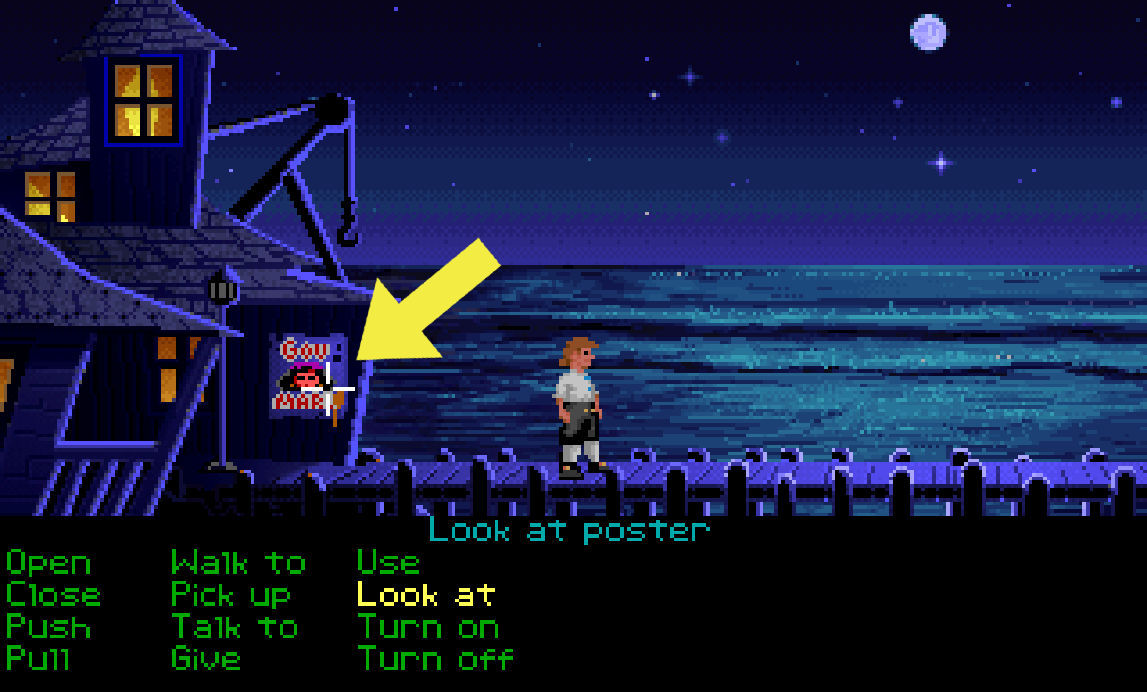
\includegraphics[width=.8\linewidth]{img/C-TSoMI.png}
\caption{The Secret of Monkey Island: Using commands and forming sentences.}
\label{fig:C-TSoMI}
\end{figure}
 
For each object in the game, there is a limited number of commands that have a meaningful result. Those that do not make sense for the given object result in the straightforward response something along the lines of “\texttt{That doesn't seem to work.}”  Then there are some that result in a humorous response, but do not help to progress the story either. And finally, certain panel actions help the player obtain a piece of information (“\texttt{Look at}”), change the state of an object (“\texttt{Open}”, “\texttt{Push}”, etc.), let them talk to a character (“\texttt{Talk to}”), or let them obtain or remove an item from the inventory (“\texttt{Pick up}” and “\texttt{Give}”).

\subsubsection{Mouse-based commands}
Some games are controlled by the mouse without the need for a panel of actions. Typically, the player clicks on an object with the mouse, and the game decides what to do based on the context. When hovering the mouse cursor over an object, a short text will pop up describing what that object is.

For example, in \textit{Beneath a Steel Sky} (see Figure \ref{fig:C-BaSS}), clicking with the right mouse button on an interactable object in the environment, the main character Foster will either pick it up or use it in some way (or talk to a character if that object was one). The same action with the left mouse button will result in the main character commenting about (e.g. describing) that object. If the player decides to use an item on an object, they must grab an icon using the right mouse button and then lead the item to the location of the object. Finally, if the player clicks on an empty spot that the main character can reach using either of the mouse buttons, Foster will move there. Overall, the game decides what the action will lead to.

\begin{figure}[H]
\centering
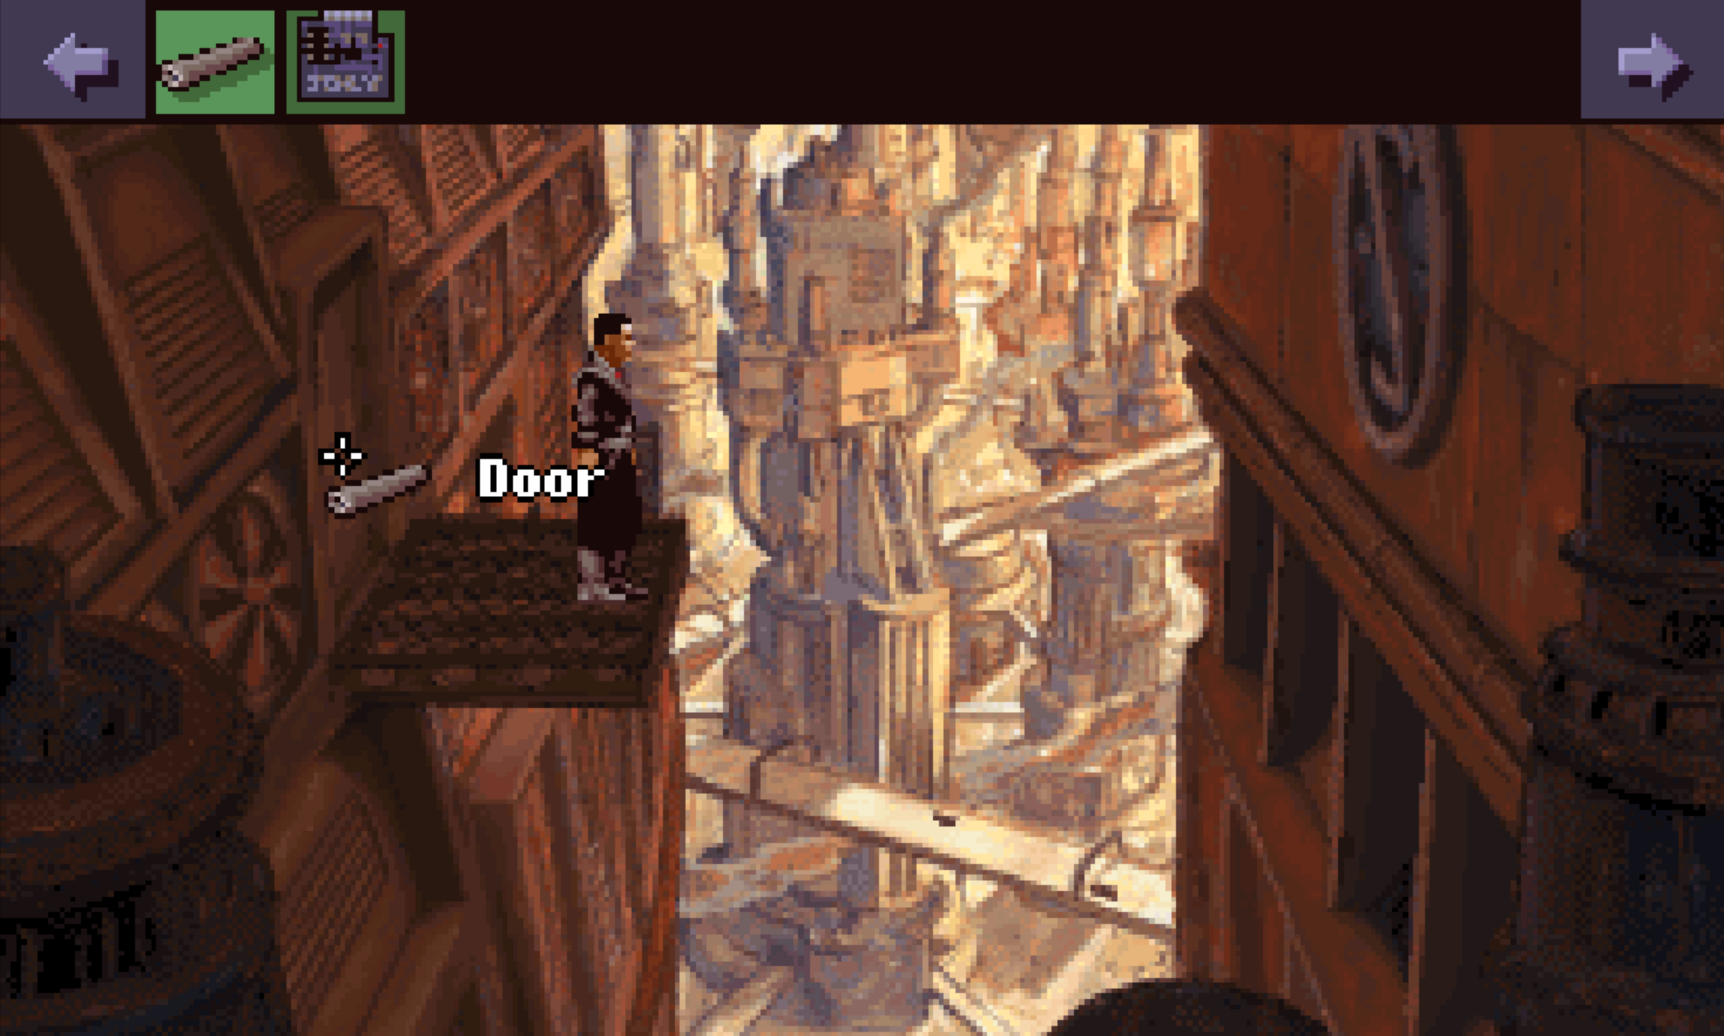
\includegraphics[width=.8\linewidth]{img/C-BaSS.png}
\caption{Beneath a Steel Sky: Using an object (a metal bar) on another object (a door).}
\label{fig:C-BaSS}
\end{figure}

\subsubsection{Requirements}
To summarize, the framework should support multiple ways for players to interact with the game's world and these are the requirements:

\begin{enumerate}[label=\color{teal}\textbf{R{\arabic*}}]
  \item \label{intro:req:com_pan} The interaction can be based on a command panel, allowing structured and predefined inputs.
  \item \label{intro:req:mouse} Alternatively, players can use direct mouse-based commands for a more intuitive and hands-on approach.
  \item \label{intro:req:mix} A game designer should be able to choose either of these methods or combine them to match different styles of gameplay.
  \end{enumerate}

\subsection{Inventory}
\label{sec:Inventory}
An inventory is an integral part of most 2D point-and-click adventure games, allowing players to store, examine, and later use items to interact with the game world. The typical visual interpretation is a panel that contains a list of items that the player had collected on their journey. These can be in the form of names, which is very distinctive for games made by Lucasfilm Games in the late 1980s and early 1990s such as \textit{Zak McKracken and the Alien Mindbenders} (1988) and \textit{The Secret of Monkey Island} (1990). Another option is to have the inventory consist of icons of items. This approach has become much more popular and can be seen in most point-and-click games.

Every game handles an inventory a bit differently. In \textit{The Secret of Monkey Island}, the inventory is always visible and is located on the right side of a panel which can be found in the lower part of the screen highlighted with purple (see Figure \ref{fig:I-TSoMI}). The inventory consists of written names of the items. 

\begin{figure}[H]
\centering
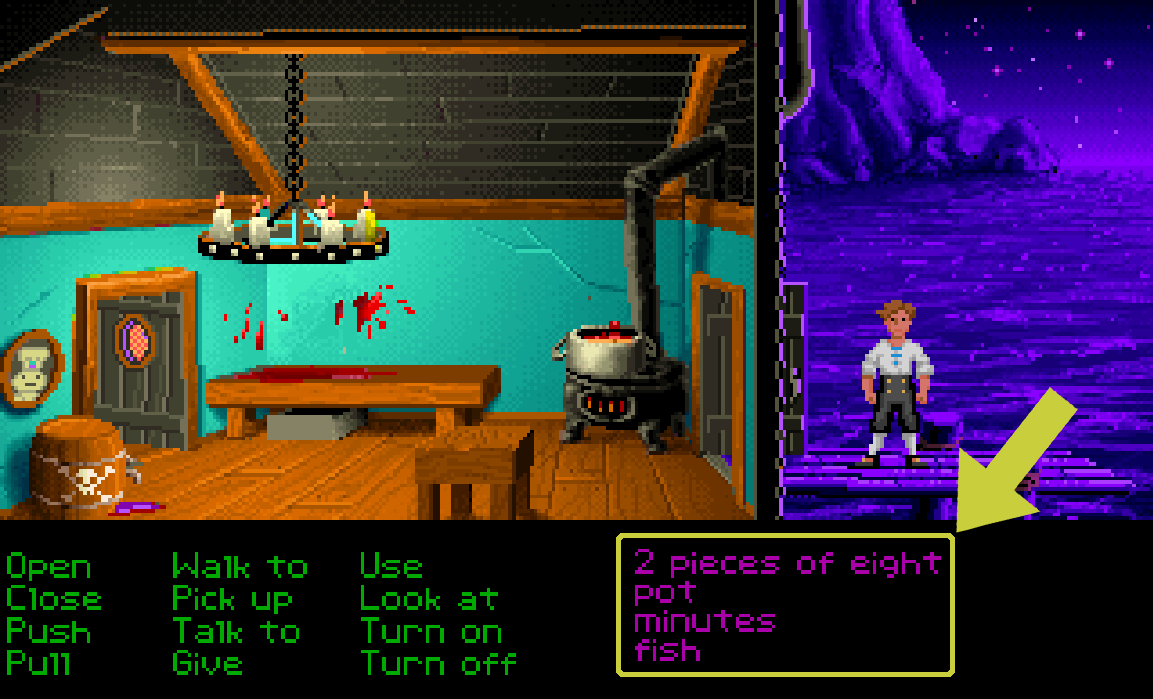
\includegraphics[width=.8\linewidth]{img/I-TSoMI.png}
\caption{The Secret of Monkey Island: Inventory.}
\label{fig:I-TSoMI}
\end{figure}

To interact with items in the inventory, the game uses the \textit{command panel} just as the rest of the environment. Although this may sound obvious, this is not always true for other games. 

\textit{Fran Bow} is an example of a more modern take on the genre while still maintaining core elements from the golden era of point-and-click adventures.  A significant difference from the previous example is the fact that the inventory is completely hidden and accessible as an independent UI element in the form of a pop-up window (see Figure \ref{fig:I-FranBow}). In the game, the inventory can be opened by clicking on an icon of a purse in the lower left corner of the screen, which then displays a panel with item icons. What is also notable about \textit{Fran Bow} is the fact that its inventory uses a different command system than the rest of the game. In the game world, the player only clicks on objects, while the inventory is controlled by three buttons, shown in Figure \ref{fig:I-FranBow}. 

\begin{figure}[H]
\centering
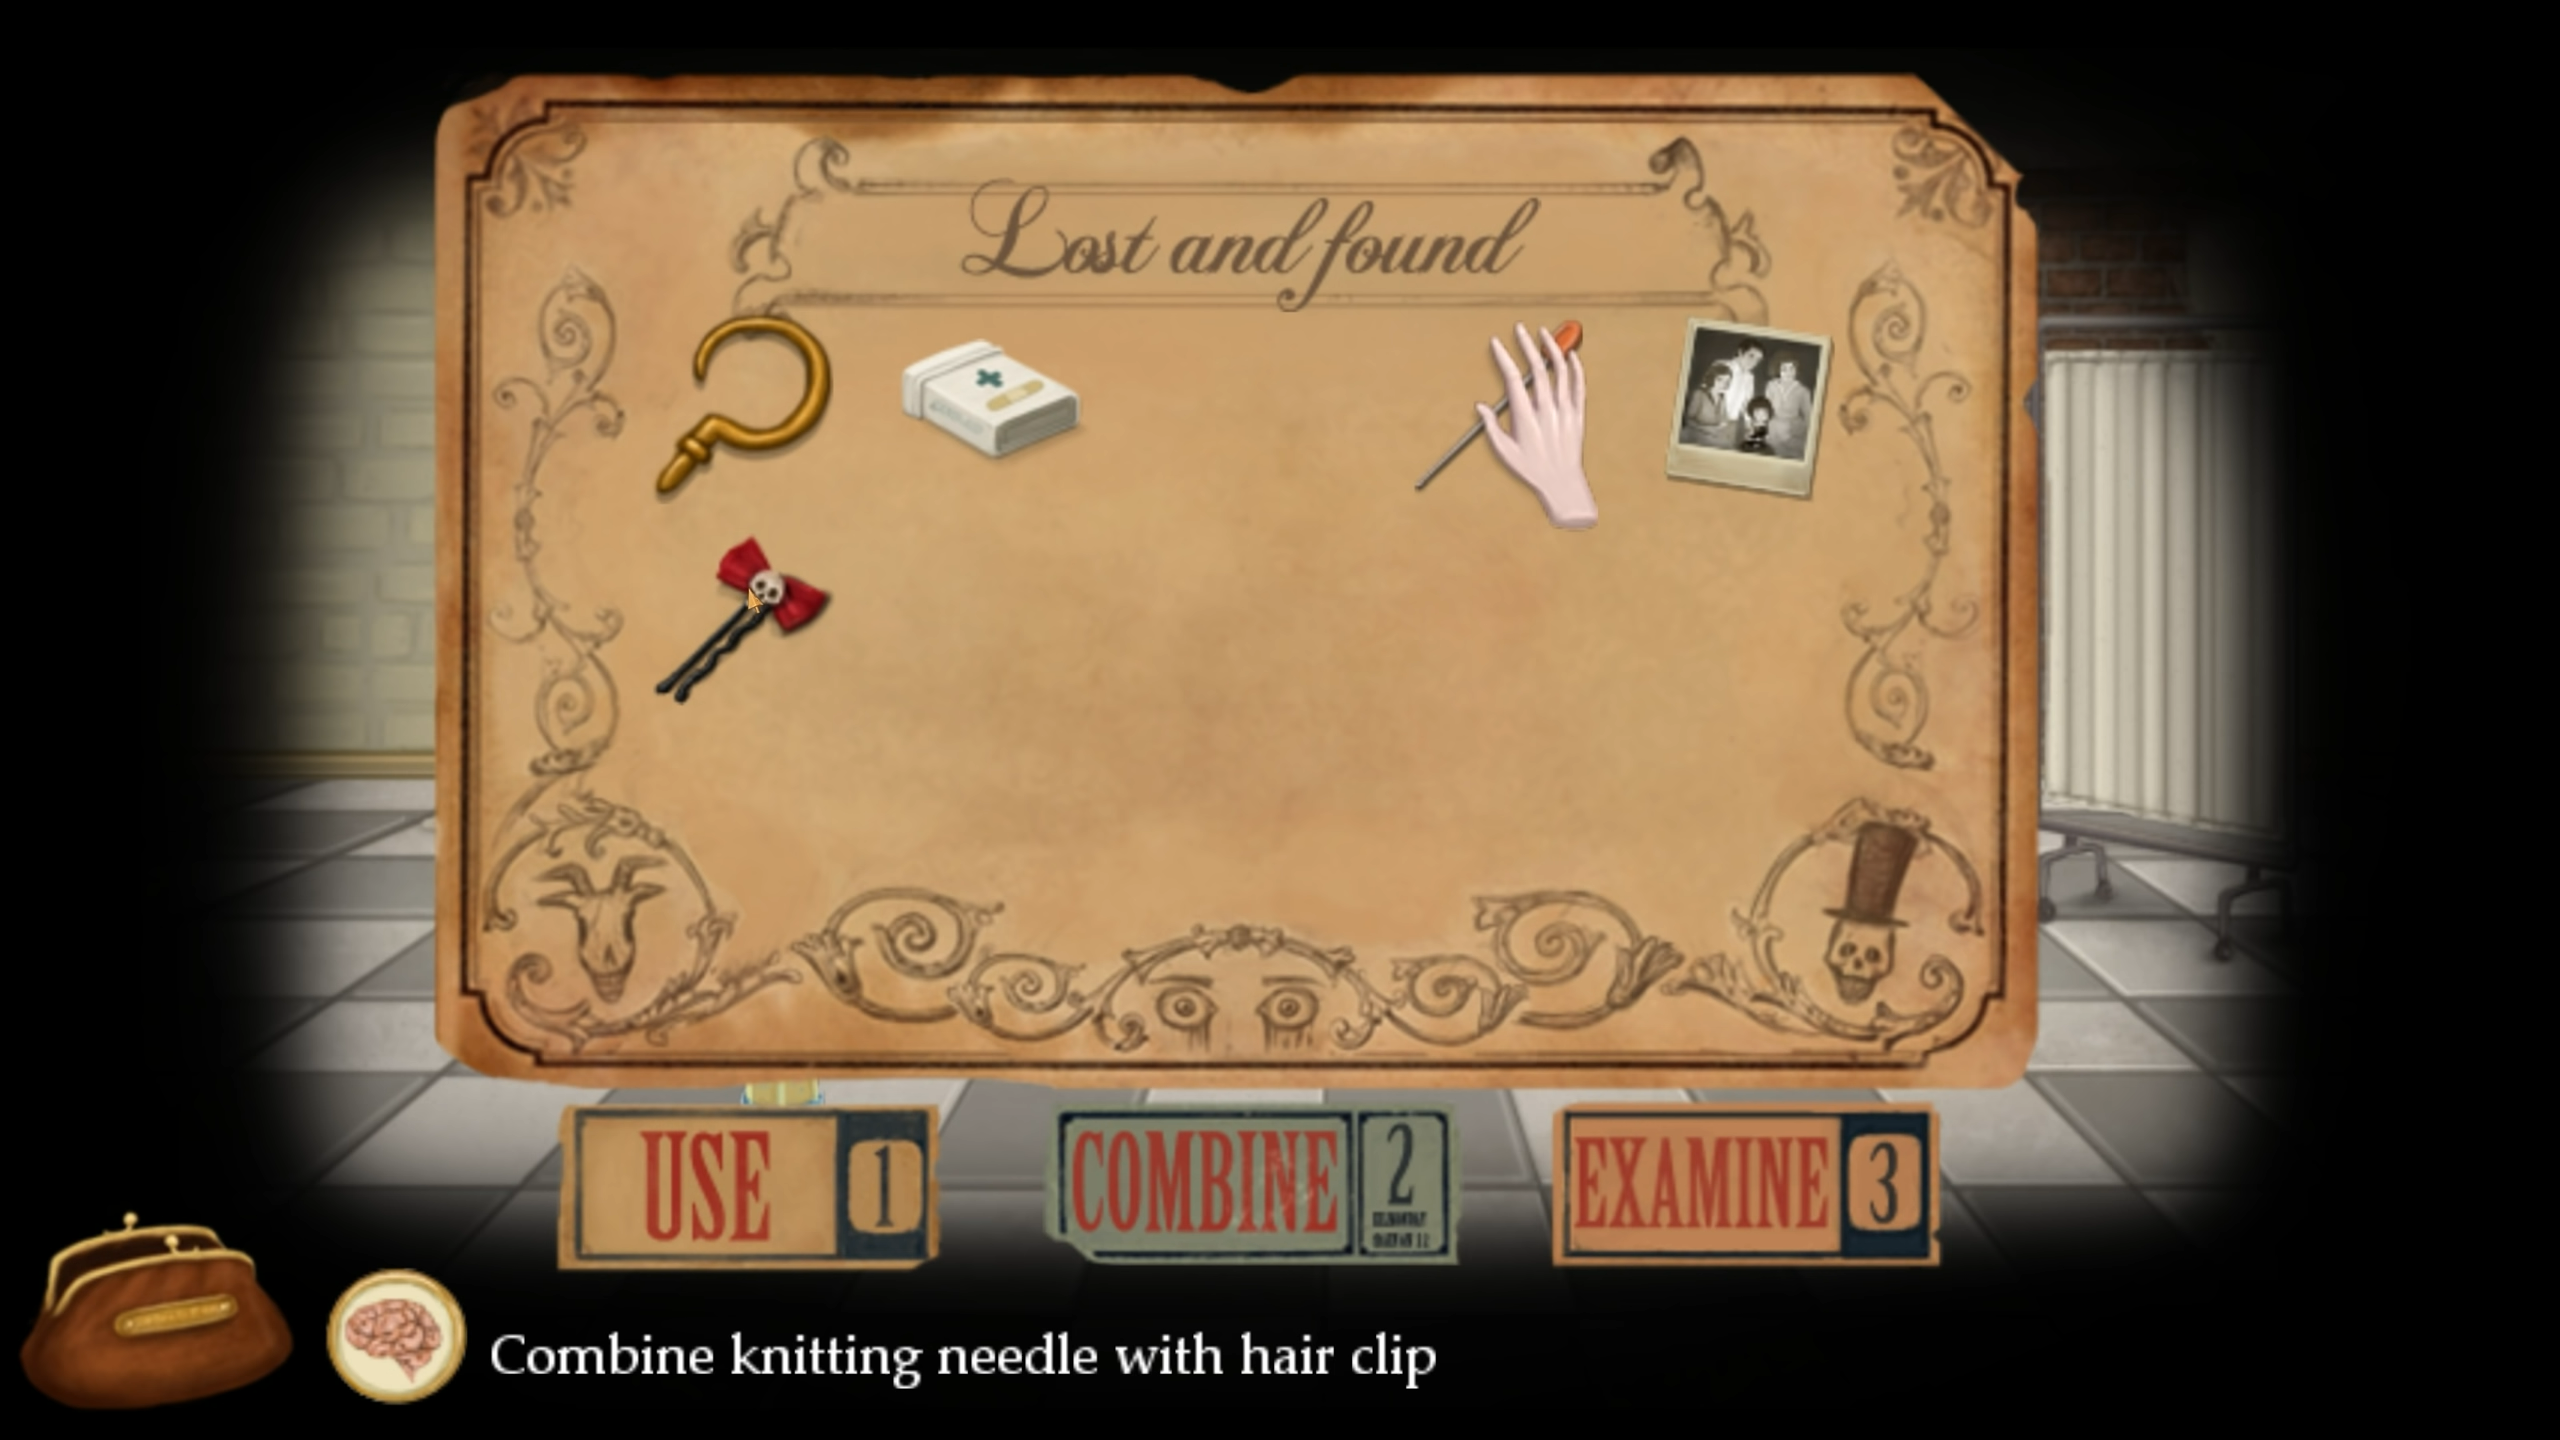
\includegraphics[width=.8\linewidth]{img/Fran_Bow.png}
\caption{Fran Bow: Inventory. Source \cite{FranBow}.}
\label{fig:I-FranBow}
\end{figure}

Although the game uses only three commands, which is a very limited number compared to other games with similar systems, these commands are considerably more versatile. When an item in the inventory is selected and “\texttt{Examine}” is pressed, the main character Fran Bow says something about the item. In addition, there is a “\texttt{Combine}” button which allows the player to choose two items and create a new one in their place within the inventory. Finally, the third button with the “\texttt{Use}” label is a bit more versatile. Depending on the item, the player can either inspect the item closer and interact with it (e.g. unlocking a locked box and finding hidden items), or use the item outside of the inventory (e.g. giving an item to another character in the game). At the bottom of the screen, a short sentence is created according to what the player will do.

Lastly, some inventories are only partially hidden, such as the one in \textit{Beneath a Steel Sky}. The player must move the mouse cursor to the top of the screen to make the inventory panel slide down. Once visible, the player can see the icons of all items in the inventory as well as their names when the mouse hovers over an icon of a metal bar, as depicted in Figure \ref{fig:I-BaSS2}. To see a longer description, the player has to click on the item with the left mouse button. The arrows on both sides of the panel are used to navigate the inventory if it contains many items.

\begin{figure}[H]
\centering
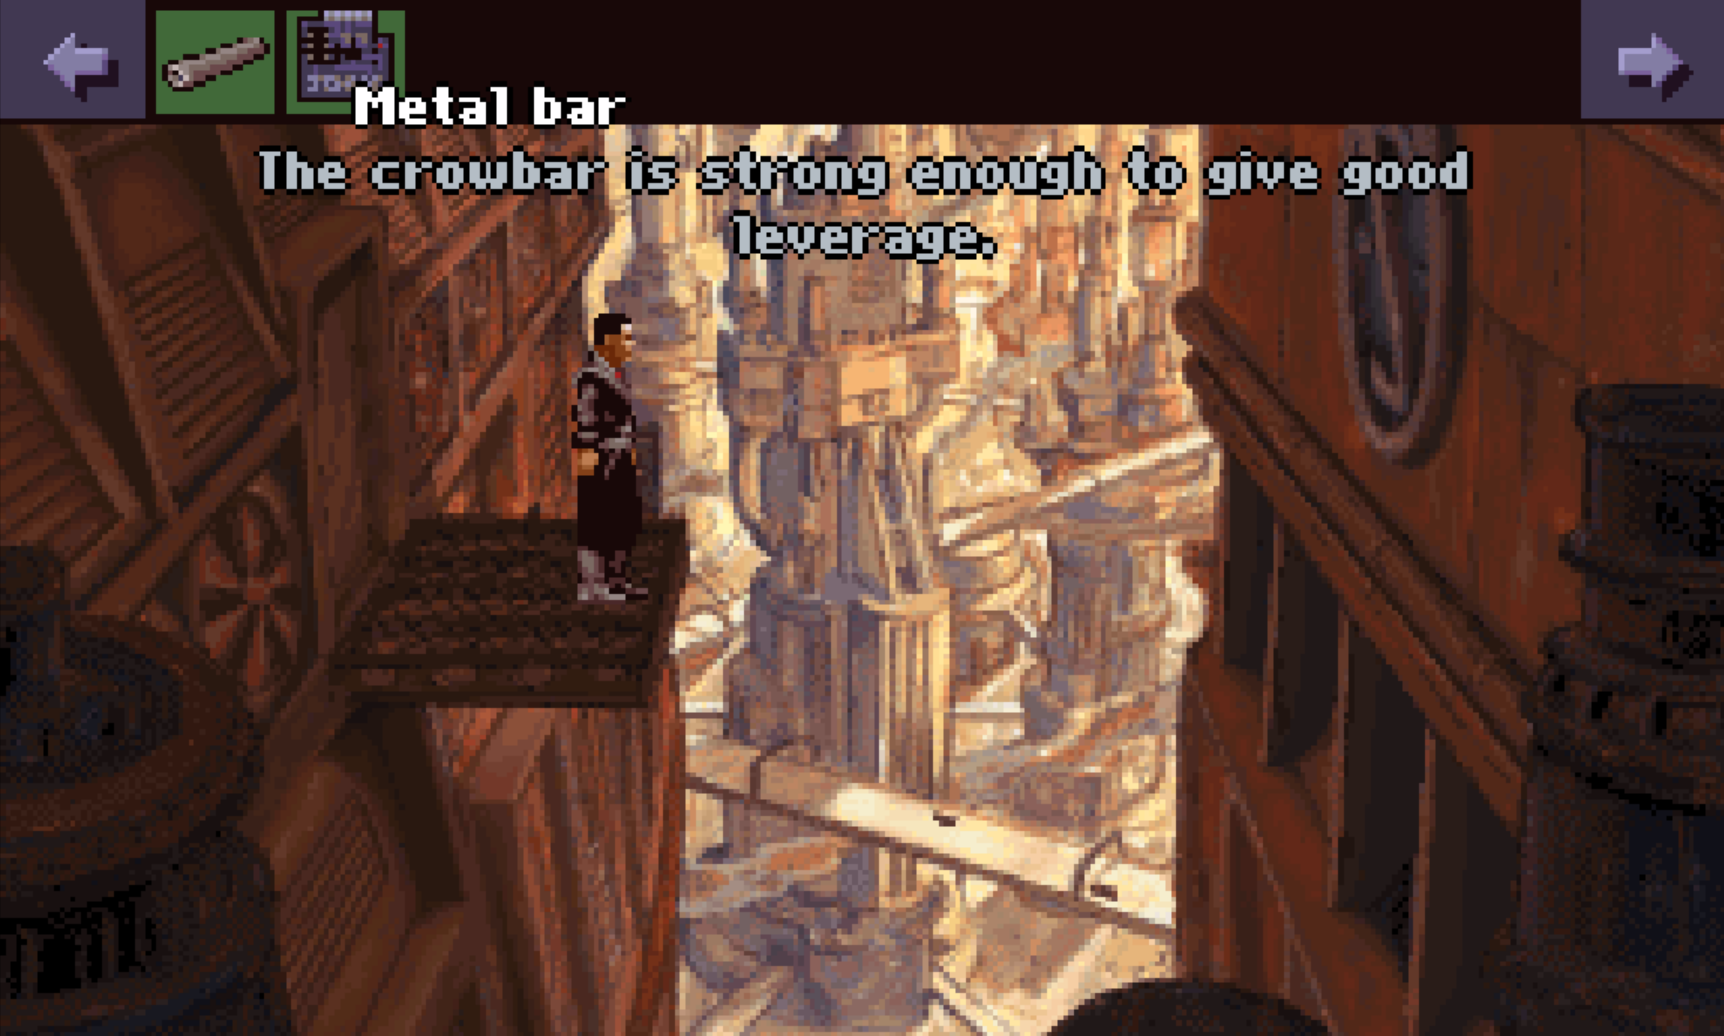
\includegraphics[width=.8\linewidth]{img/I-BaSS2.png}
\caption{Beneath a Steel Sky: Displaying a tag with the name of the item in white and a short description in grey.}
\label{fig:I-BaSS2}
\end{figure}

\subsubsection{Requirements}
It is clear that the approach of games from the point-and-click genre to an inventory is very varied. That is why we want to give developers the freedom to implement it their own way by developing an inventory system that is easy to integrate and customize. In summary, here are the requirements:

\begin{enumerate}[label=\color{teal}\textbf{R{\arabic*}},resume]
  \item \label{intro:req:inv_formats} The system should support multiple inventory formats, such as static, pop-up, or sliding inventories.
  \item \label{intro:req:text_icon} Both text-based lists and icon-based layouts should be available as inventory options.
\end{enumerate}

\subsection{Character movement}
\label{sec:Character movement}
Exploration of the in-game world is achieved through character movement. A typical way to achieve this is by clicking on a location in the environment, which prompts the character to find the shortest path and move there. The way movement is implemented can greatly impact the player's sense of control and immersion. Some games incorporate command buttons to refine the movement system. Additionally, other techniques, like character scaling, help create the illusion of depth in a 2D space to immerse the player into the game's world.

\subsubsection{Types of control}
As outlined in the previous sections, the main two ways of controlling a character either involve or do not involve the use of a command button. The one in \textit{The Secret of Monkey Island} is a prime example of the use of a command button. To move the character to another position, one must select the “\texttt{Walk to}” button and then click on a point in the environment that is not occupied by any object, as seen in Figure \ref{fig:M-TSoMI-W}. In case an object stands in that place, the character will just walk to the object without interacting with it. If there does not exist a path to the given point, the character will find the closest position to that point and walk there.

\begin{figure}[H]
\centering
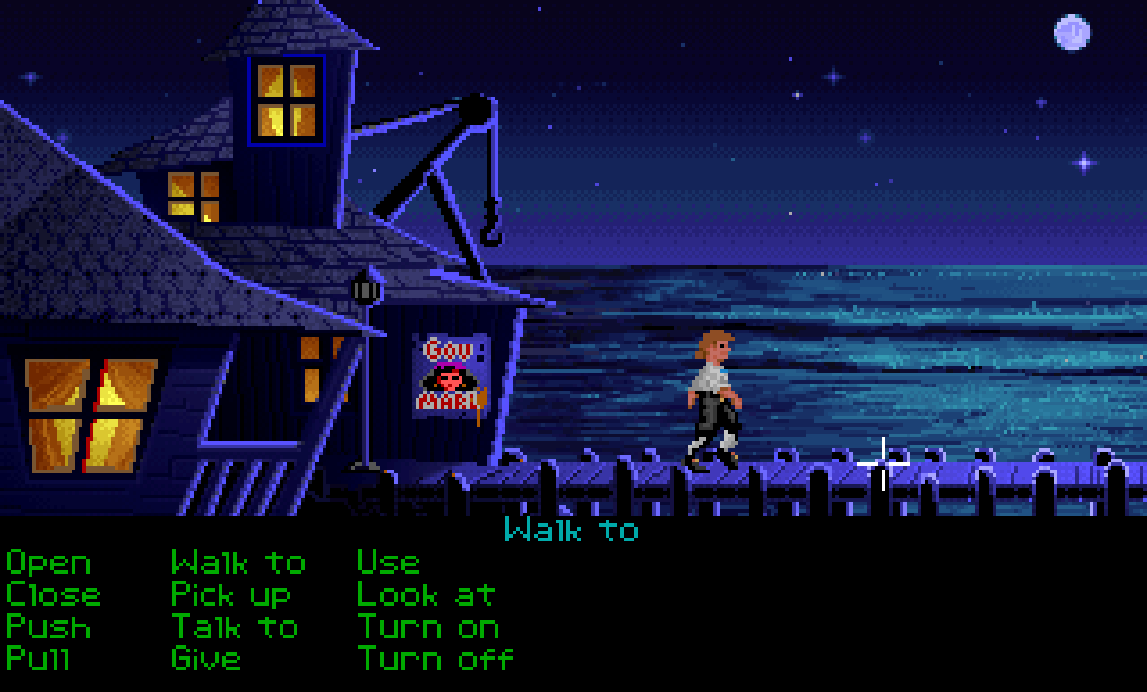
\includegraphics[width=.8\linewidth]{img/W-TSoMI.png}
\caption{The Secret of Monkey Island: Walking to a point where the mouse cursor is located.}
\label{fig:M-TSoMI-W}
\end{figure}

To move the character to another position, the second option involves just clicking on a point in the environment with a mouse that is not occupied by any object as seen in Figure \ref{fig:M-BaSS}. If a point occupied by an object is selected, the main character will not only walk to the point but will also interact with it.

\begin{figure}[H]
\centering
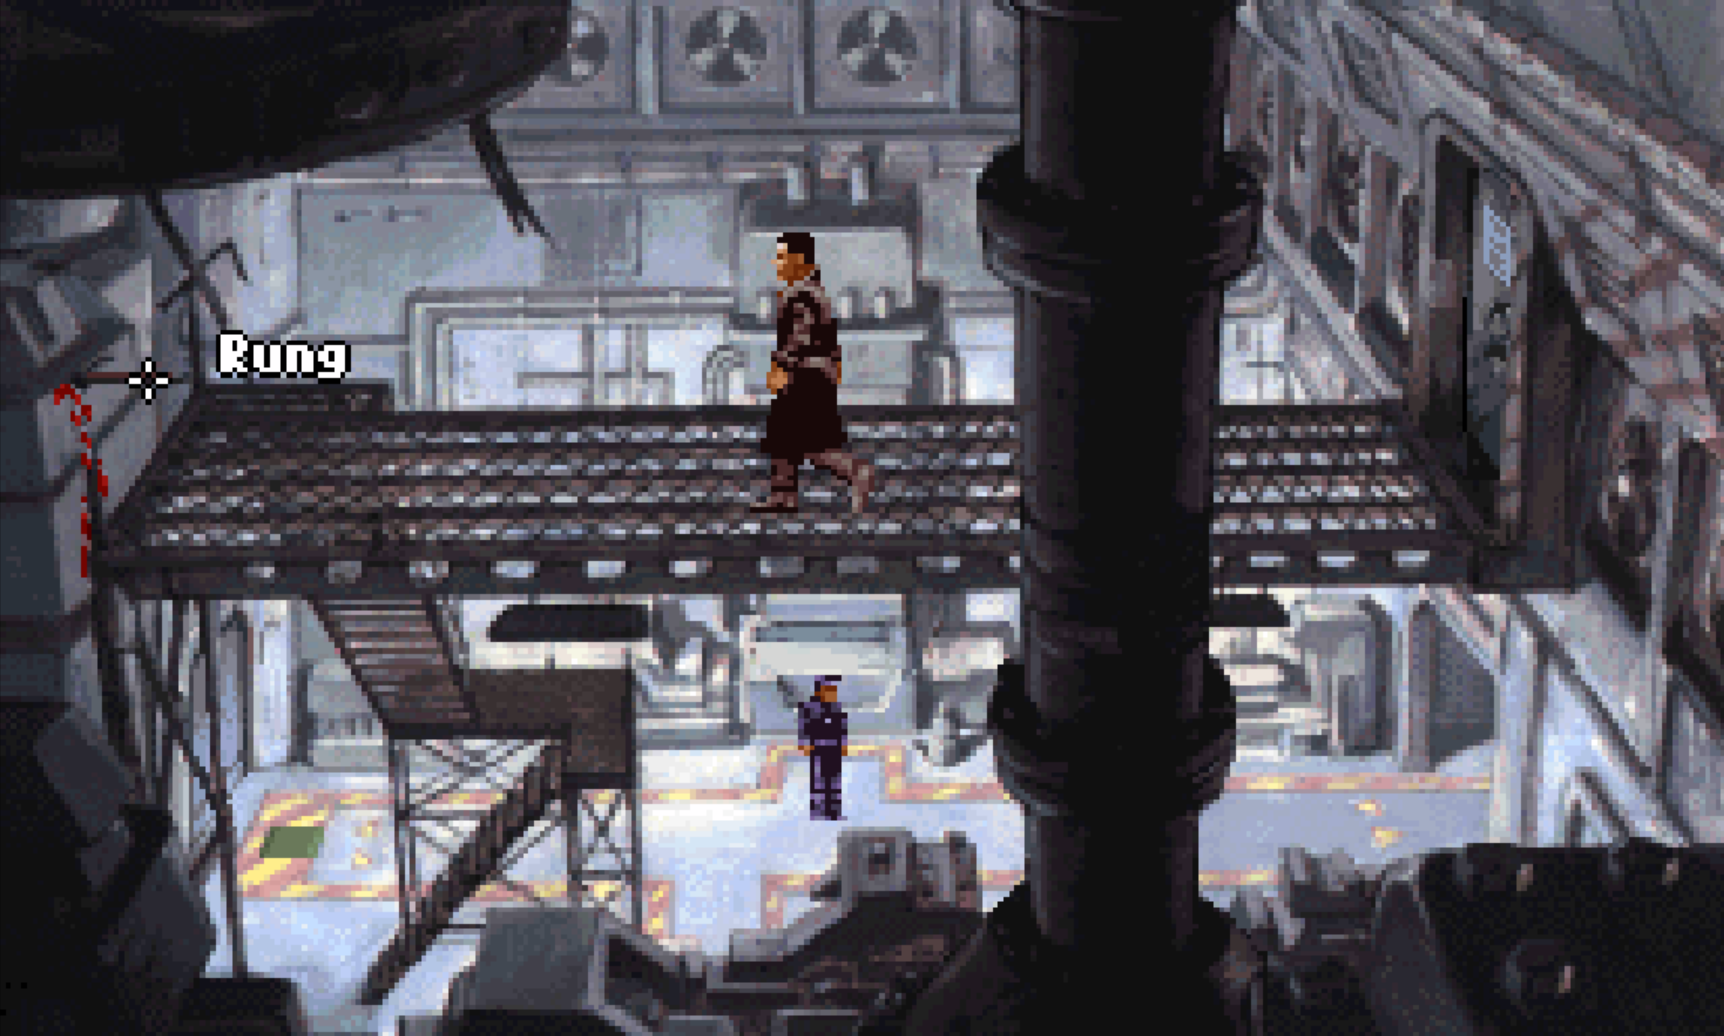
\includegraphics[width=.8\linewidth]{img/M-BaSS.png}
\caption{Beneath a Steel Sky: Walking to an object (a rung).}
\label{fig:M-BaSS}
\end{figure}

%\vspace{5mm}
\textbf{Requirements} \quad In the framework, the character movement system supporting multiple interaction methods and intelligent navigation has the following requirements:

\begin{enumerate}[label=\color{teal}\textbf{R{\arabic*}},resume]
  \item \label{intro:req:com+mouse_move} Both command-based movement (e.g. selecting a “\texttt{Walk to}” button) and direct mouse-based movement (clicking on a location) should be supported.
  \item \label{intro:req:mox_move} Developers should have the option to define whether clicking on an object triggers only movement or both movement and interaction.
  \item \label{intro:req:pathfinding}Pathfinding should be incorporated so characters can automatically navigate around obstacles to reach their destination.
\end{enumerate}

\subsubsection{Depth simulation}
In some point-and-click adventure games, perspective elements are incorporated to enhance depth and spatial awareness. 
A very notable feature in some games that enhances the feeling of a 3D space is the inclusion of layers. Since the scenes in 2D point-and-click adventure games are not (usually) made using 3D spaces, the games have to simulate the appearance of objects being obscured by other objects. The difficult part comes when objects move around the scene. At one point, a character can be standing in front of an object, and then they can be standing behind the object. This means that first the character needs to be drawn above the object, and later they need to be drawn below it, just as in Figure \ref{fig:M-TSoMI0}.

\begin{figure}[H]
\centering
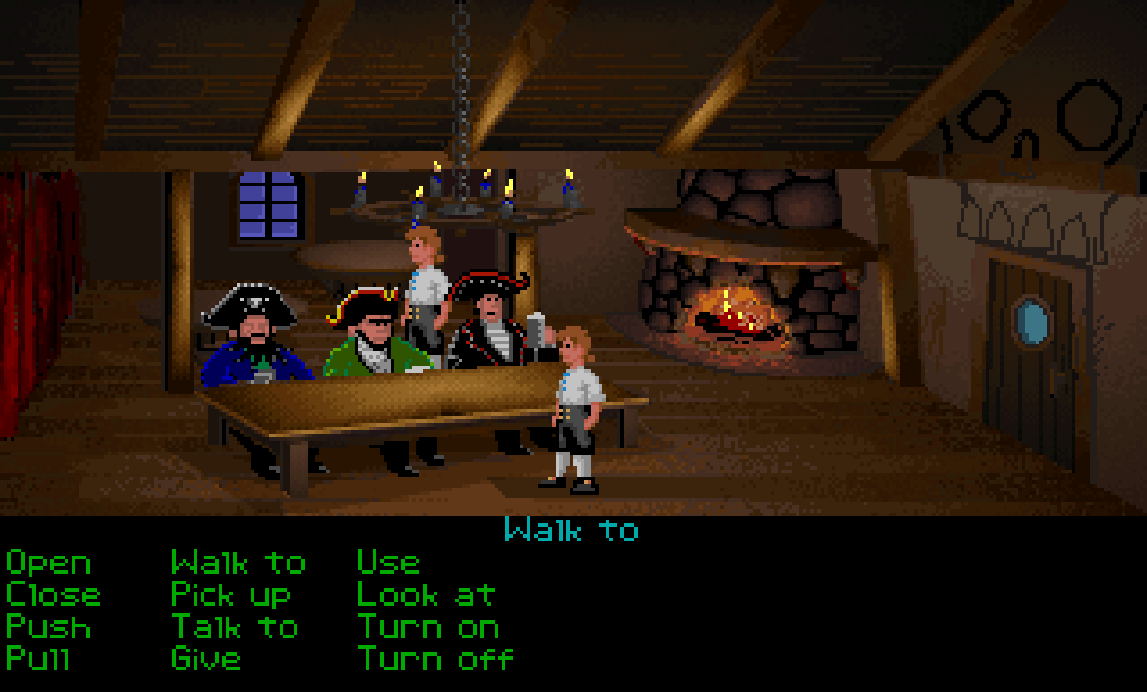
\includegraphics[width=.8\linewidth]{img/M-TSoMI0.png}
\caption{The Secret of Monkey Island: Layered composition of a 2D scene.}
\label{fig:M-TSoMI0}
\end{figure}

Another way to create the illusion of a three-dimensional space within a 2D environment is making characters appear smaller as they move into the distance. One of the best examples representing this feature is in the starting area of \textit{The Secret of Monkey Island} where the main protagonist walks along the cliffside and gradually increases in size, as shown in Figure \ref{fig:M-TSoMI}. This effect can help establish a sense of scale and immersion, making the game world feel more dynamic and visually engaging. 

\begin{figure}[H]
\centering
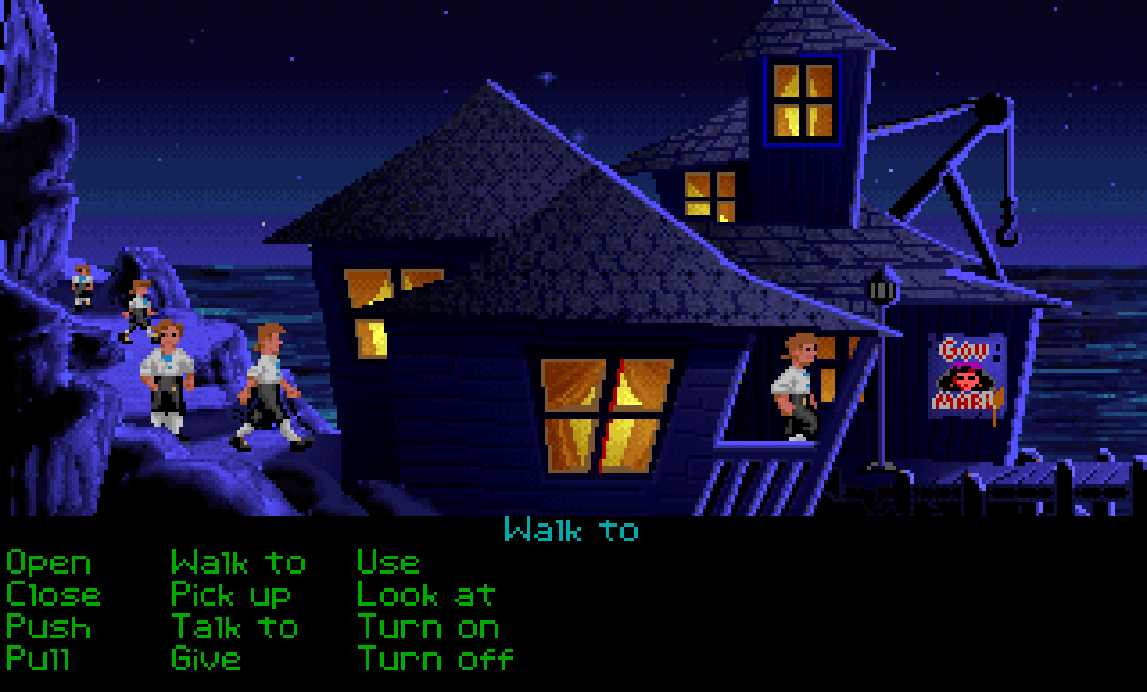
\includegraphics[width=.8\linewidth]{img/M-TSoMI.png}
\caption{The Secret of Monkey Island: Perspective simulation.}
\label{fig:M-TSoMI}
\end{figure}

A similar effect was also achieved in \textit{Beneath a Steel Sky} where the main protagonist walks down a set of stairs while also being partially obscured by the platform above, which is depicted in Figure \ref{fig:M-BaSS0}. Upon closer inspection, it appears that this is achieved in the form of a cutscene, as the player is unable to interact with the game. For example, the player cannot change the direction the character heading to when he reaches the staircase up until he exits it. 

\begin{notImplemented}
\quad {\footnotesize \textit{(not implemented)}} \par
\vspace{3mm}
Cutscenes are sequences during which usually the player cannot interact with the game. Its main goal is mostly to show an even or a transition from one scene to another. Although cutscenes are widely used across various game genres, this framework will not include them, as they fall outside the scope of this project.
\end{notImplemented}

\begin{figure}[H]
\centering
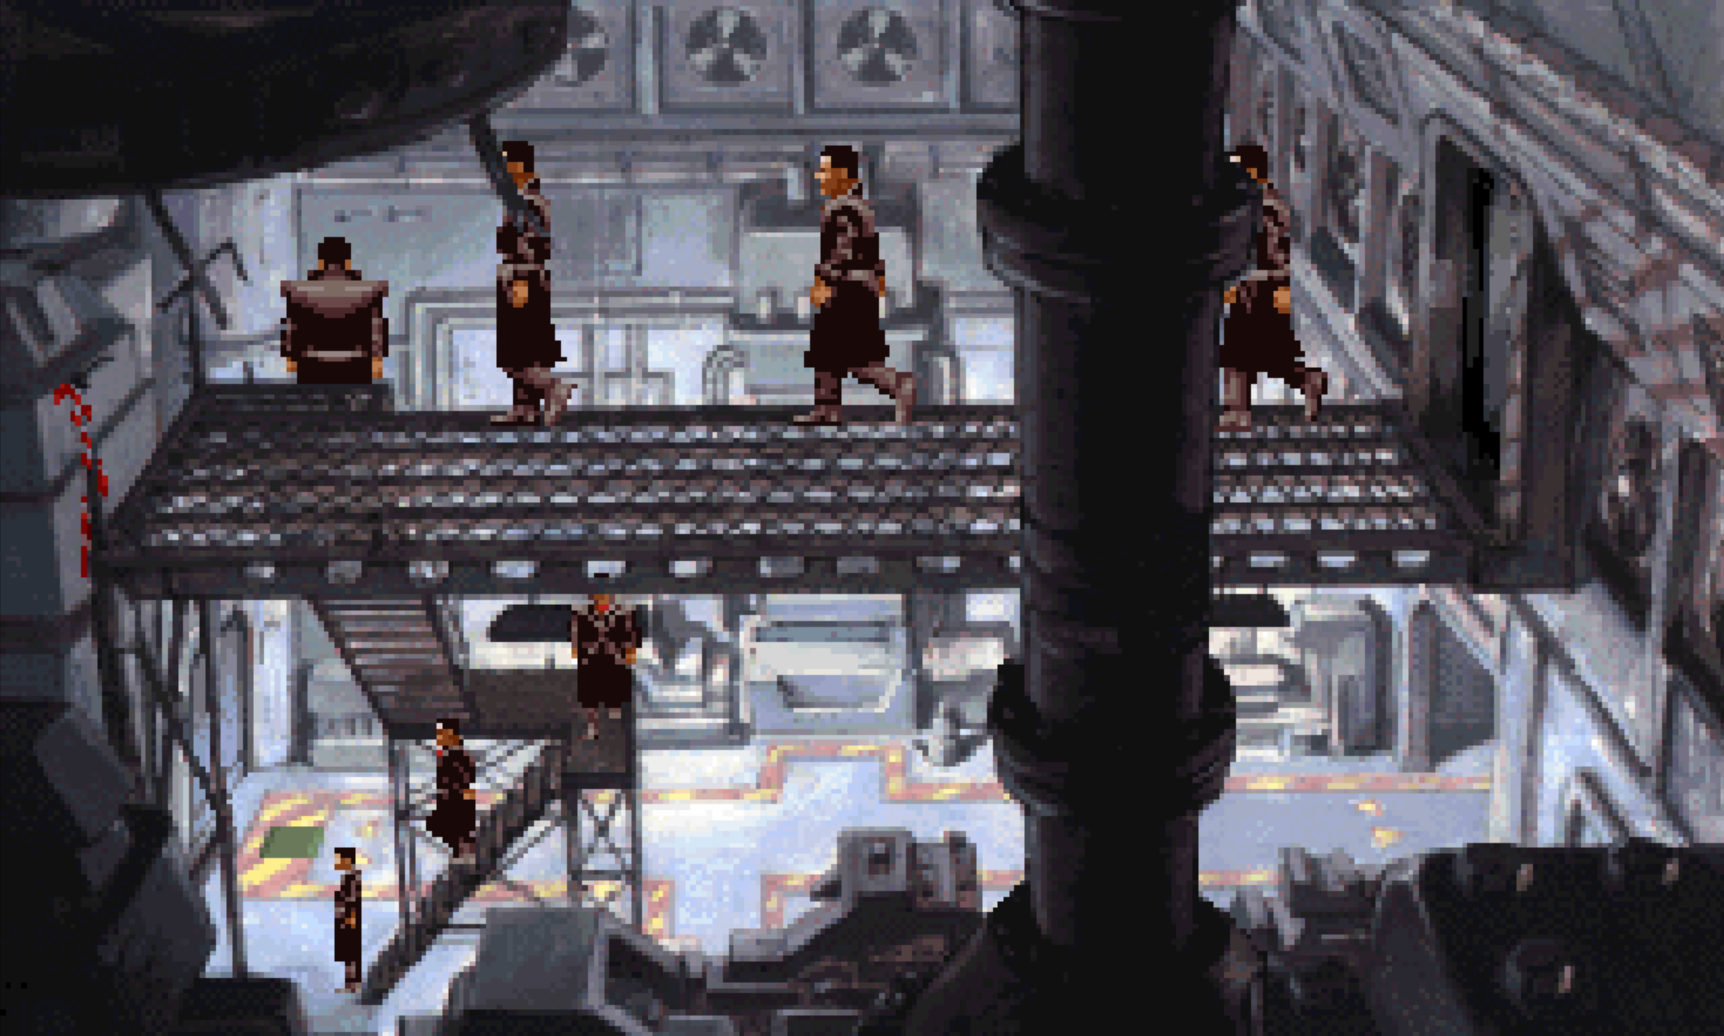
\includegraphics[width=.8\linewidth]{img/M-BaSS00.png}
\caption{Beneath a Steel Sky: Perspective simulation.}
\label{fig:M-BaSS0}
\end{figure}

%\vspace{5mm}
\textbf{Requirements} \quad In summary, the illusion of depth enables the player to immerse themselves into the game's world and is achieved by the following:

\begin{enumerate}[label=\color{teal}\textbf{R{\arabic*}},resume]
  \item \label{intro:req:scale} Characters should dynamically scale to enhance depth perception.
  \item \label{intro:req:layers} Characters should adjust their position in front of or behind objects to preserve the 3D effect and to ensure a more natural and immersive experience.
\end{enumerate}
    
\subsection{Dialogue}
\label{sec:Dialogue}
Dialogues are a very important part of a 2D point-and-click game. In some examples, it is more advanced, with many options to choose from (\textit{The Secret of Monkey Island}), and in others its structure is more simple (\textit{Fran Bow}).  

In the following paragraph, we refer to terms \textit{dialogue mode} and \textit{gameplay mode} to describe how the game handles conversations. These are not standard definitions of game design. Instead, they describe the state of the games based on our observations. To initialize a dialogue with an NPC in \textit{The Secret of Monkey Island}, the player must first enter the \textit{dialogue mode} by selecting the “\texttt{Talk to}” command and then clicking on them, as shown in Figure \ref{fig:D-TSoMI0}. When done so, the dialogue starts and some features, such as the inventory, are inaccessible. Instead, the player can choose an option on how to respond to the NPC (see Figure \ref{fig:D-TSoMI1}). 

\begin{figure}[H]
\centering
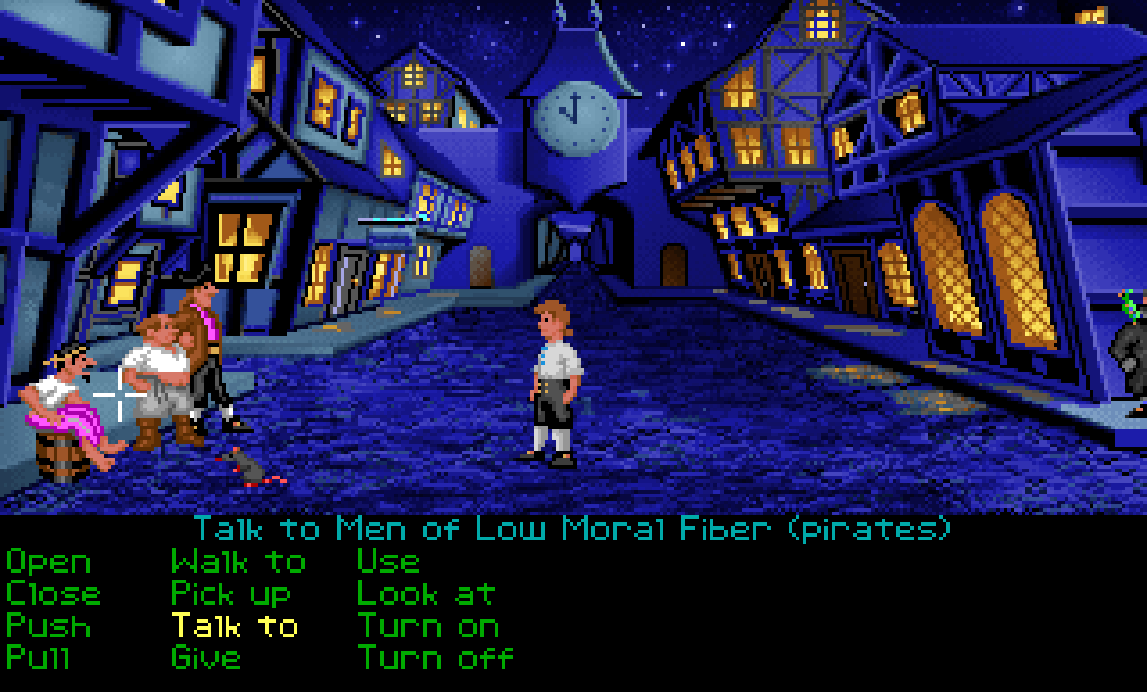
\includegraphics[width=.8\linewidth]{img/D-TSoMI0.png}
\caption{The Secret of Monkey Island: Before starting a conversation.}
\label{fig:D-TSoMI0}
\end{figure}

\begin{figure}[H]
\centering
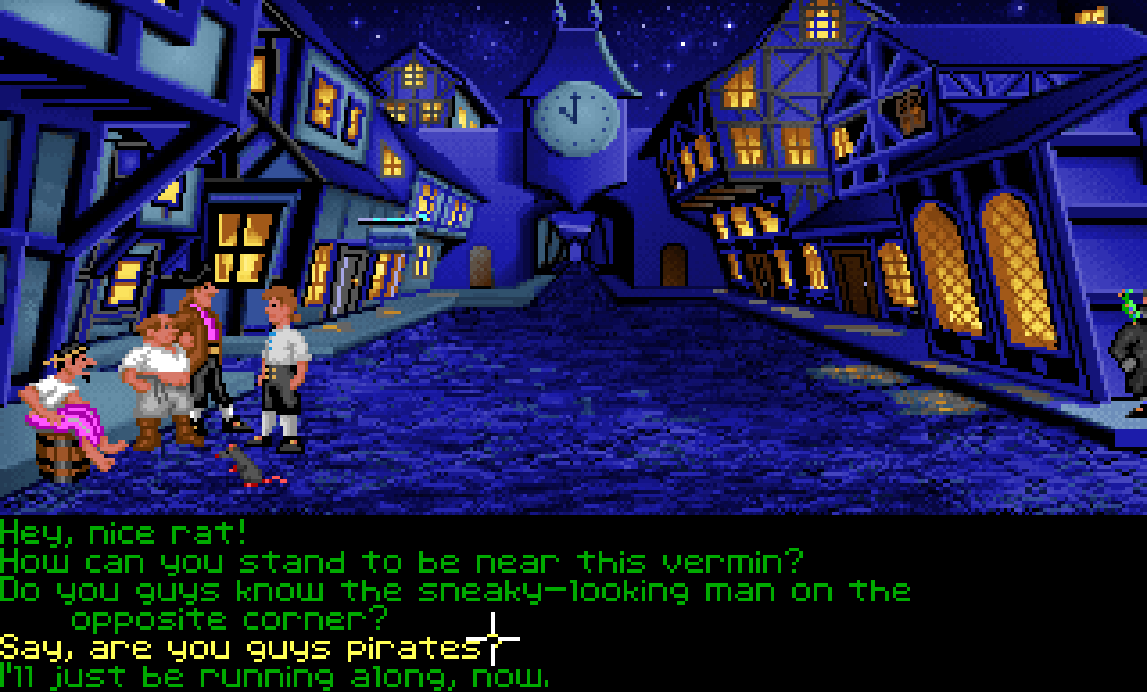
\includegraphics[width=.8\linewidth]{img/D-TSoMI1.png}
\caption{The Secret of Monkey Island: Dialogue options in a conversation.}
\label{fig:D-TSoMI1}
\end{figure}

By selecting the option, the player responds, and the dialogue continues until the player has the option to choose an answer again. Typically, subtitles are used to make the dialogue more accessible and understandable even with limited audio, this can be observed in Figure \ref{fig:D-TSoMI2}. To exit \textit{dialogue mode}, a specific option must be selected, and the player is back in \textit{gameplay mode}.

\begin{figure}[H]
\centering
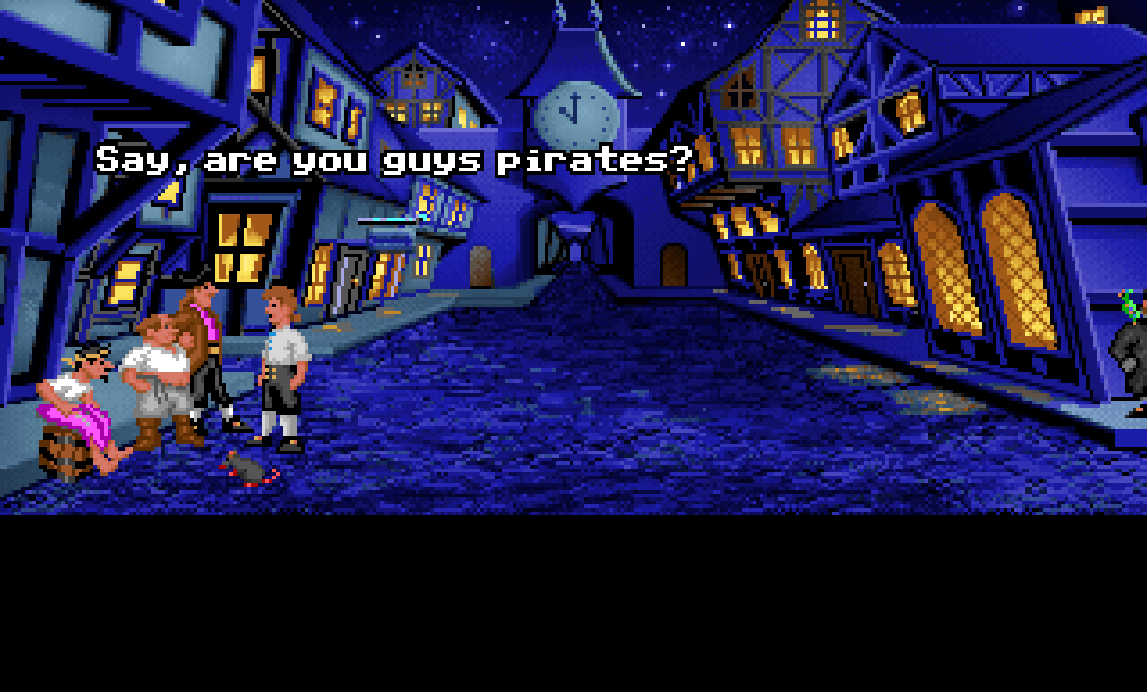
\includegraphics[width=.8\linewidth]{img/D-TSoMI2.png}
\caption{The Secret of Monkey Island: Conversation displayed through subtitles.}
\label{fig:D-TSoMI2}
\end{figure}

\textit{Fran Bow} uses a similar approach. When the player clicks on an NPC, the dialogue mode is activated. As seen in Figure \ref{fig:D-FranBow}, they can interact by choosing one of two options displayed in the bottom panel. In addition, subtitles appear in bubbles above the heads of the characters. 

\begin{figure}[H]
\centering
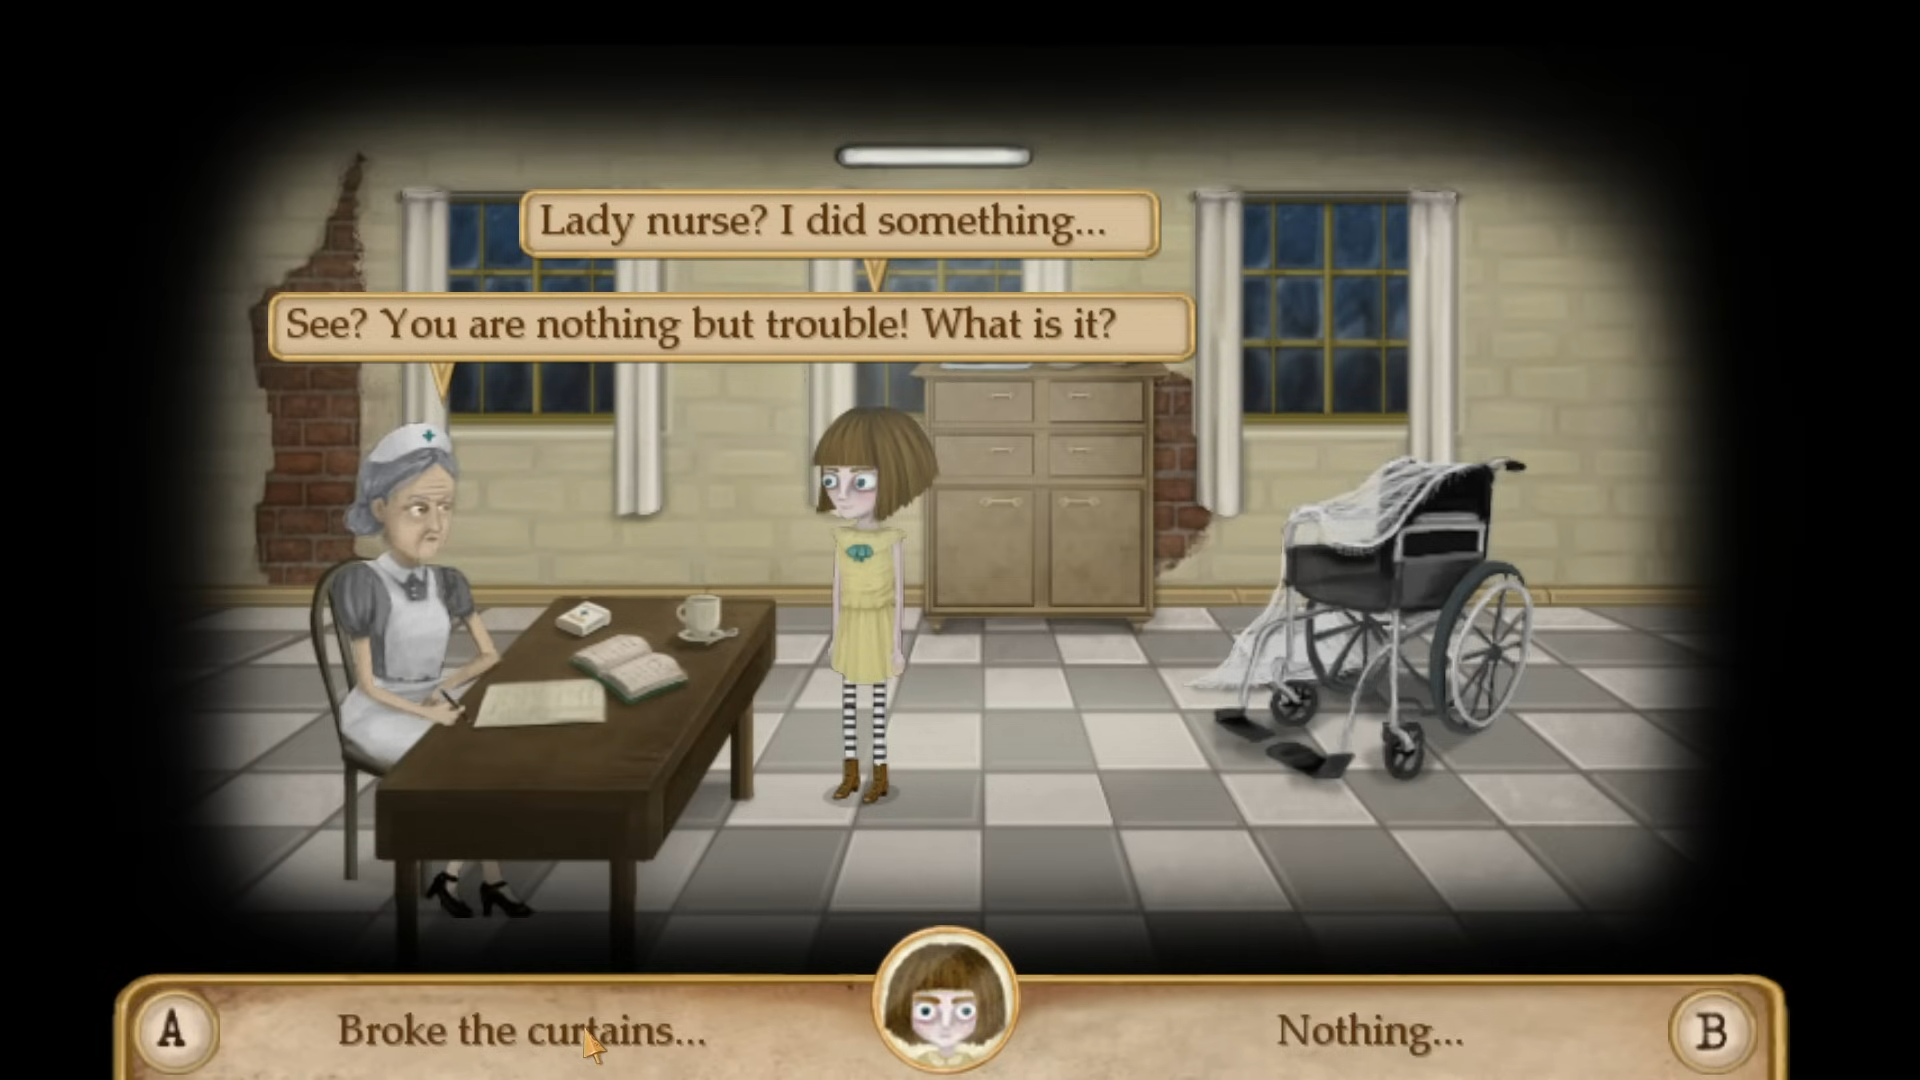
\includegraphics[width=.8\linewidth]{img/D-FB.png}
\caption{Fran Bow: Conversation with an NPC. Source \cite{FranBow}.}
\label{fig:D-FranBow}
\end{figure}

In these two examples, the NPCs were static, so to talk to them, the character must approach them. However, this is not always the case. When examining \textit{Beneath a Steel Sky} a bit closer, one may notice that the NPCs move quite a lot around the environment and this includes also the characters player can talk to. This means that the main character must meet the character at some point on the map. \textit{Beneath a Steel Sky} solves it by determining a fixed point where the player character and the NPC must go and start the conversation depicted in Figure \ref{fig:C-BaSS3}. When the player initiates a conversation with the NPC wearing pink, they are standing in positions \texttt{A} and \texttt{C} respectively. Afterwards, the characters move to positions \texttt{B} and \texttt{D} where they start with the conversation.
%\todo{include this in the project?}

\begin{figure}[H]
\centering
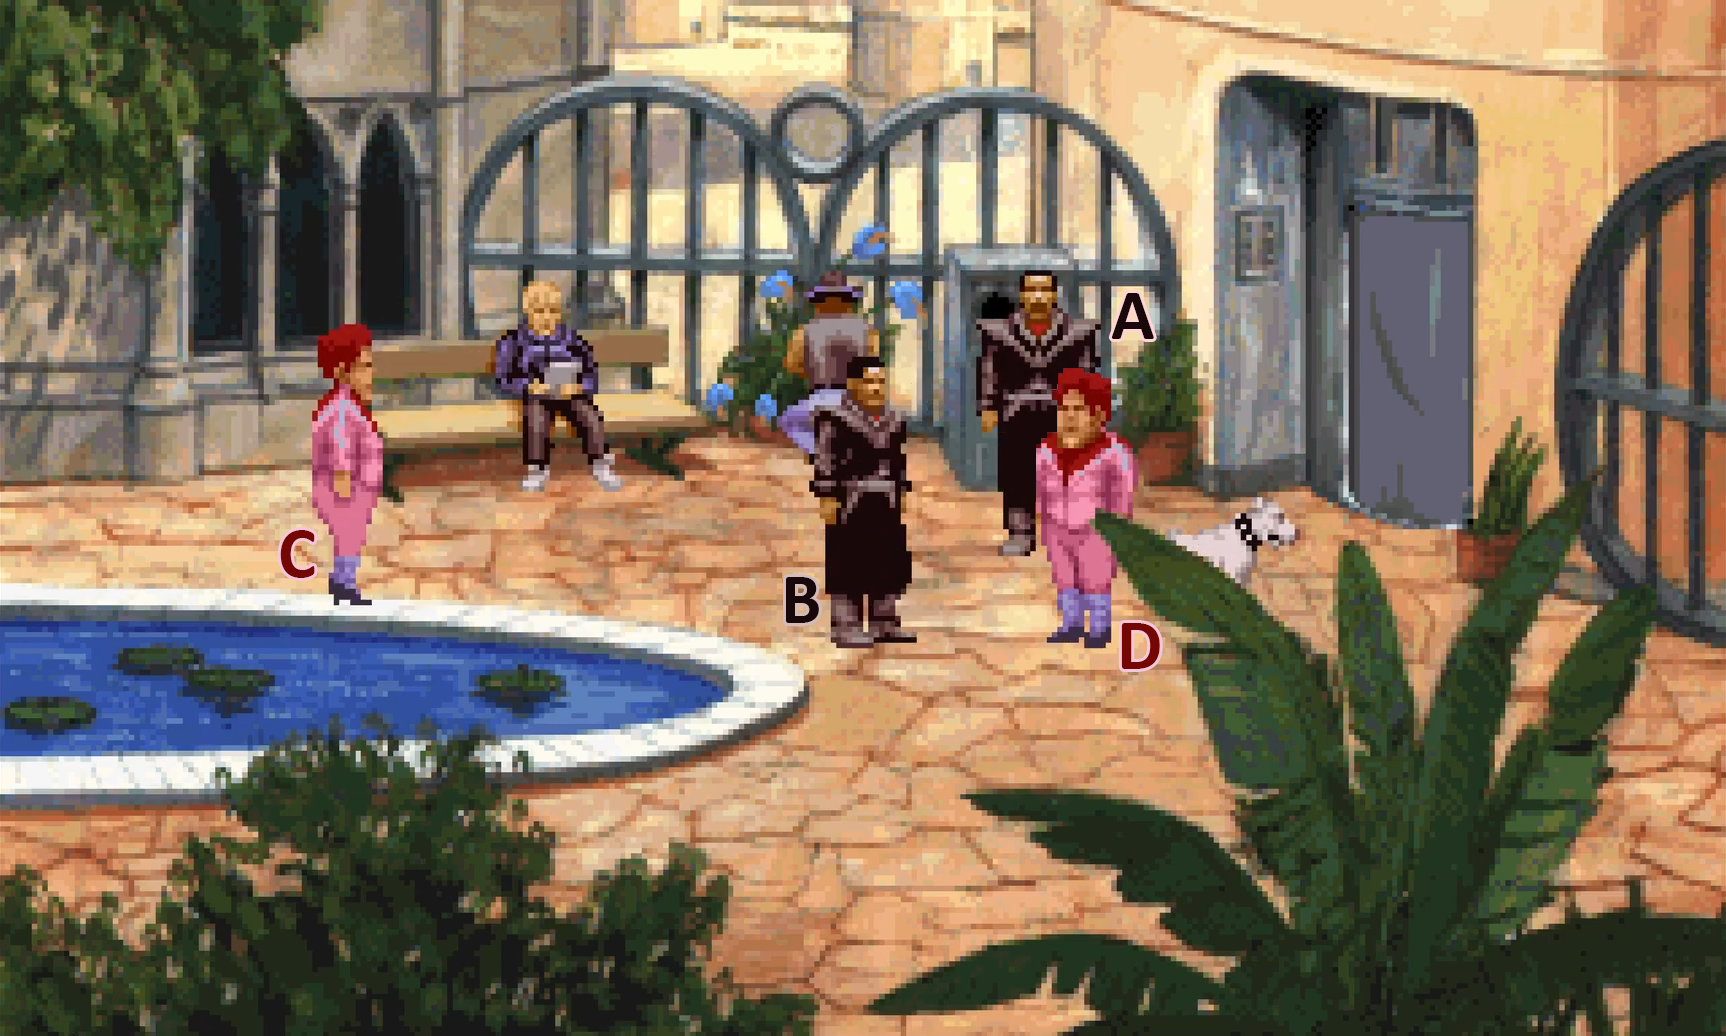
\includegraphics[width=.8\linewidth]{img/C-BaSS2.png}
\caption{Beneath a Steel Sky: Conversation with a moving NPC.}
\label{fig:C-BaSS3}
\end{figure}

\subsubsection{Requirements}
To summarize, these are the rules the dialogue system should follow:

\begin{enumerate}[label=\color{teal}\textbf{R{\arabic*}},resume]
  \item \label{intro:req:multi_dialogue} It should allow for complicated branching conversations with multiple-choice dialogue options.
  \item \label{intro:req:modes} There should be a clear distinction between dialogue mode and gameplay mode, restricting interactions like inventory access during conversations.
  \item \label{intro:req:subs} Subtitles should be included to improve accessibility and player comprehension, regardless of audio availability.
  \item \label{intro:req:sub_format} Different visual styles for dialogue presentation should be supported, such as text in a dedicated panel or speech bubbles above characters.
\end{enumerate}


\subsection{Animation}
\label{sec:Animation}
A video game may contain thousands of objects, but without animation, the world feels lifeless.  To achieve the effect of a moving object in 2D point-and-click game, typically images called sprites are played closely after one another.  Figure \ref{fig:A-TSoMI} shows a small sample of sprites that the game \textit{The Secret of Monkey Island} (1990) used for the main character.

\begin{figure}[H]
\centering
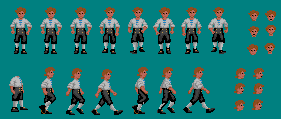
\includegraphics[width=.65\linewidth]{img/AN-TSoMI2.png}
\caption{The Secret of Monkey Island: Sprite sheet of the main character.}
\label{fig:A-TSoMI}
\end{figure}

\begin{notImplemented}
\quad {\footnotesize \textit{(not implemented)}} \par
\vspace{3mm}
As shown, animation is a very important aspect of a game. Despite that, we will not implement a system for animation into the framework as it is a feature that exceeds the scope of the bachelor thesis and is not crucial to showcase the concept of a point-and-click toolkit. It is a feature that would be implemented in the future.
\end{notImplemented}

\subsection{Sound System}
\label{sec:Sound_Management}
A soundtrack and sound effects are an integral part of every video game, be it a mobile game or a console game. They not only set the mood and immerse the player in the game's world, but also help them navigate the environment. For example, while exploring, a player might hear the sound of flowing water, guiding them toward a new area near a river. If a sound system is missing in a game, it is very striking to even a novice player. 

\begin{notImplemented}
\quad {\footnotesize \textit{(not implemented)}} \par
\vspace{3mm}
Although the inclusion of sound effects and a soundtrack is very important in every game, this framework will not include them, as they are not a crucial feature in the base of the framework we are designing. Naturally, if we were to push the project further and if we wanted to finalize the project, the inclusion of a sound management system would be a necessity.
\end{notImplemented}

\subsection{Mini-games}
\label{sec:Minigames}
Finally, many 2D point-and-click adventure games include features that cannot be considered staples of the genre, one of those being mini-games. They can be best described as games within games and usually fall outside the norms of a typical point-and-click gameplay. When a player starts a mini-game, core gameplay features, such as the inventory and the walking systems, are disabled and replaced with mechanics tailored to the mini-game’s unique interactions.  A perfect example is \textit{Fran Bow}, which features a wide variety of mini-games. In Figure \ref{fig:UF-FB1}, the player must solve a puzzle by reassembling the tiles so that all the gears turn. Later, the player guides a frog across the water by jumping on logs and other floating objects, which closely resembles the classic 1981 arcade game \textit{Frogger}, as seen in Figure \ref{fig:UF-FB2}. 

\begin{figure}[H]
\centering
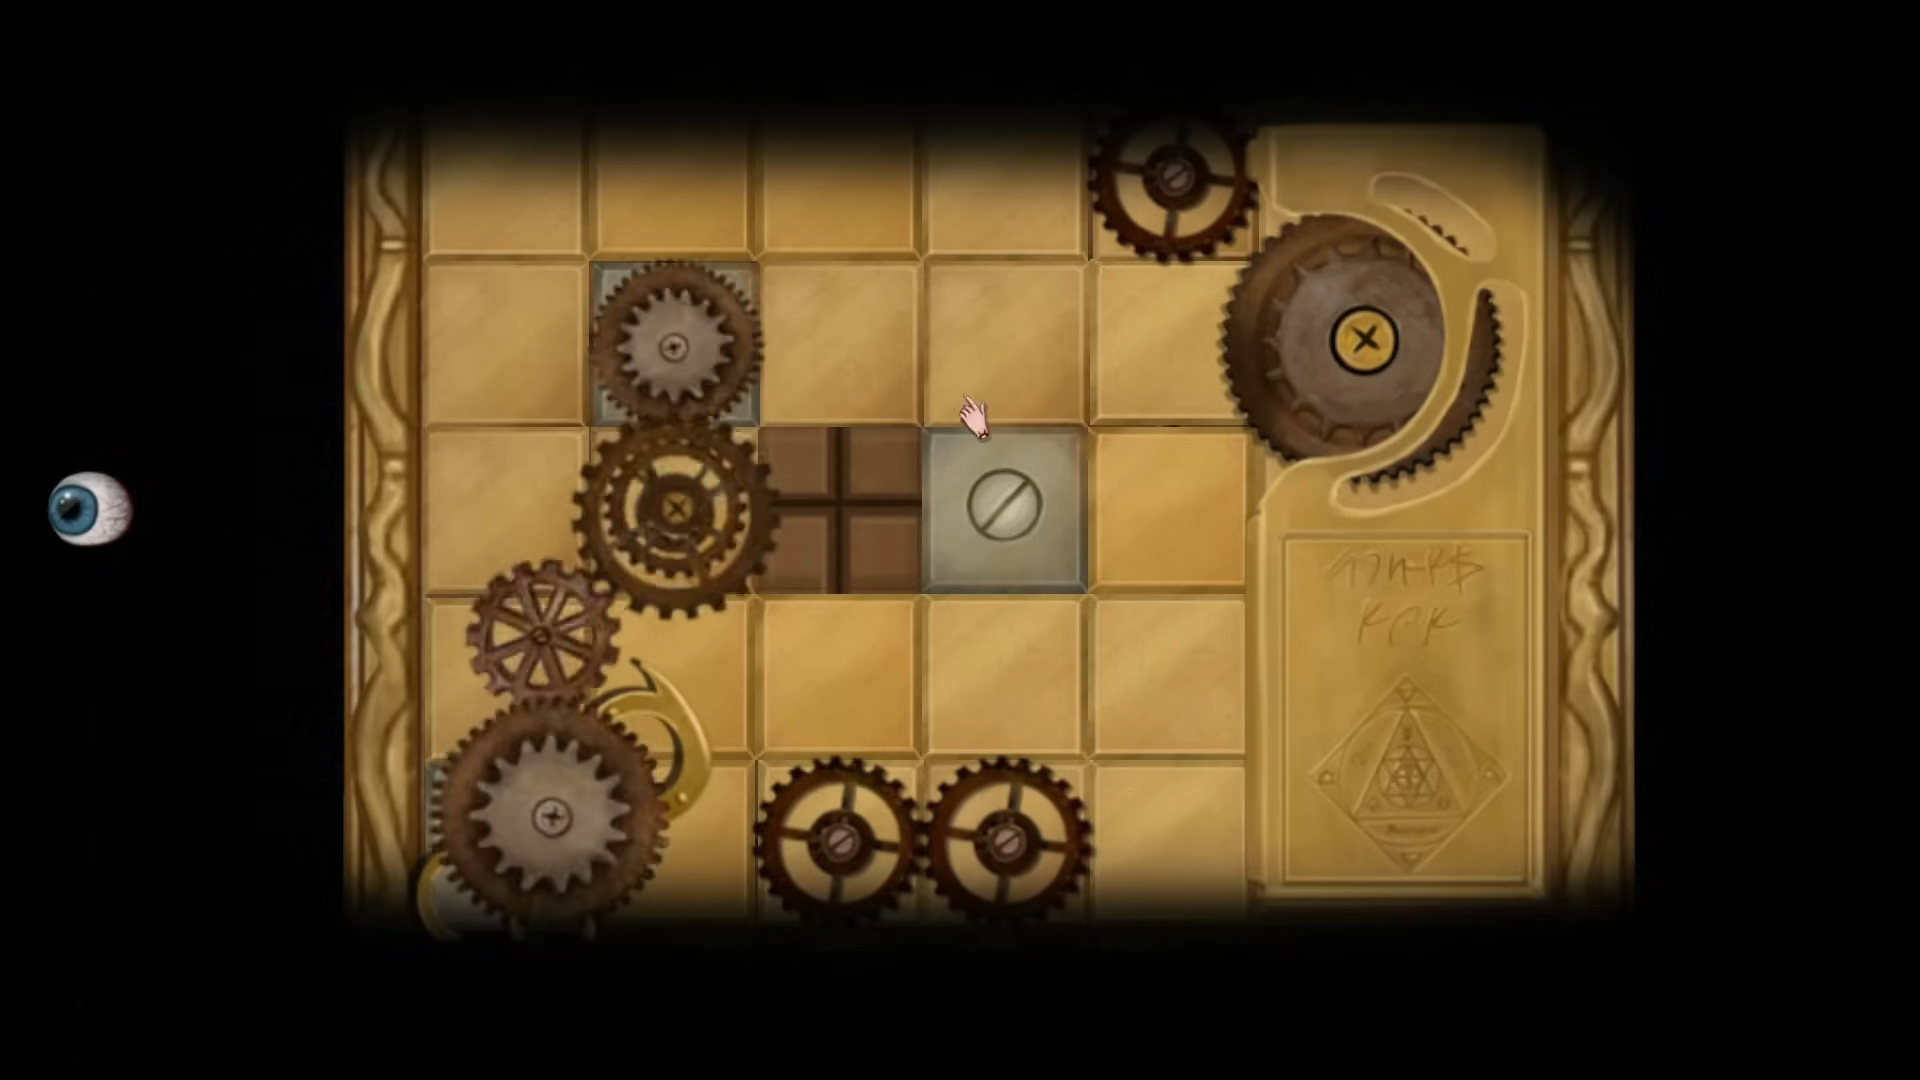
\includegraphics[width=.8\linewidth]{img/FB_BF1.png}
\caption{Fran Bow: Gear reassembling mini-game. Source \cite{FranBow}.}
\label{fig:UF-FB1}
\end{figure}

\begin{figure}[H]
\centering
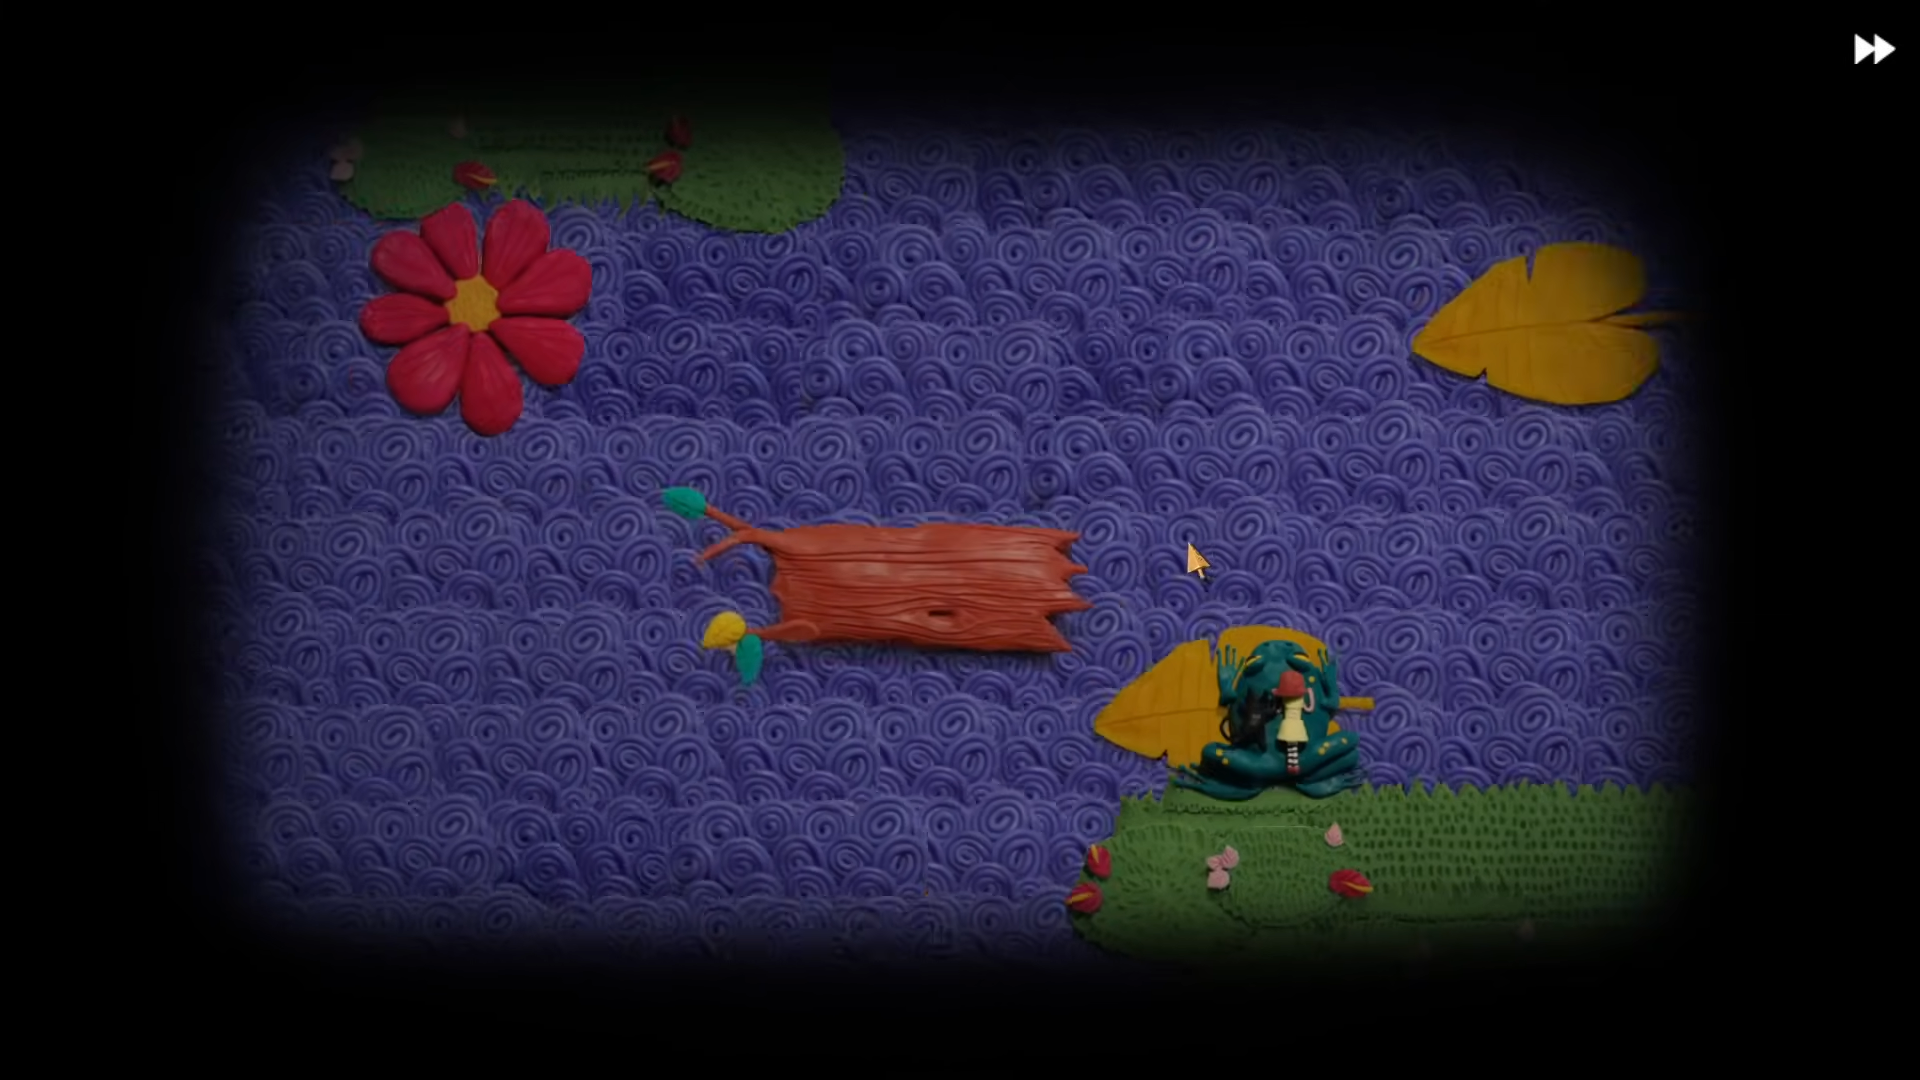
\includegraphics[width=.8\linewidth]{img/FB_BF2.png}
\caption{Fran Bow: Frogger mini-game. Source \cite{FranBow}.}
\label{fig:UF-FB2}
\end{figure}

\begin{notImplemented}
\quad {\footnotesize \textit{(not implemented)}} \par
\vspace{3mm}
Game developers take inspiration from various genres and are not restricted by the norms of just one. On one hand, this makes games unique and intriguing, but on the other, it makes creating a system for such a feature very challenging, as it is impossible to predict what a developer might want to implement. That is why this is outside the scope of the project, and the framework will not include it. 
\end{notImplemented}


\section{Showcase}
\label{intro:showcase}
Outside the framework itself, another goal of the thesis is to showcase the implemented features. This will be achieved by making a game that only consists of certain scenes from a few 2D point-and-click games recreated using our framework. The scenes will include:
\begin{itemize}
    \item \textit{The Secret of Monkey Island} (1990)
    \item \textit{Beneath a Steel Sky} (1994)
\end{itemize}

\section{Goals}
\label{intro:goals}
\begin{enumerate}[label=\color{orange}\textbf{G{\arabic*}}]
  \item \label{intro:goals:framework} 
  Design a framework in the Unity game engine \textit{TaleCraft} satisfying requirements \ref{intro:req:com_pan}--\ref{intro:req:sub_format}.
  \item \label{intro:goals:demo} Create a demo game consisting of scenes from different games of the 2D point-and-click adventure genre outlined in Section \ref{intro:showcase}.
\end{enumerate}

\chapter{Unity Engine}
\label{chap:refs}
Unity is a cross-platform development environment widely used to build interactive applications, particularly video games. Its support for the C\# programming language, combined with extensive official documentation and a wealth of community-created tutorials, makes it highly accessible to developers of various experience levels. Our framework will be implemented in Unity using version 2022.3.61f1. 

This chapter introduces essential Unity development concepts that form the foundation for the rest of the thesis. While experienced Unity users may already be familiar with this material, others can refresh their memory on basic concepts. For those who want to learn more, they are encouraged to study the Unity manual \cite{Unity-manual} for more in-depth information. 

\section{Scenes}
Unity organises game content into units called \textit{scenes}, which commonly represent individual levels, menus, or other distinct game states. Developers can freely switch between these scenes, each serving as a workspace in which the game environment is built by placing and configuring various elements, referred to as \textit{GameObjects}. 

\section{GameObjects}
In Unity, all entities present within a scene are instances of the class \verb|GameObject|. This includes a wide range of elements such as characters, environmental props, cameras, lighting, and visual effects. A \verb|GameObject| serves as a fundamental container that represents an object in the scene. However, by itself, it does not possess any visual appearance or behaviour.

\subsection{Parenting}
\verb|GameObjects| can be organised hierarchically by assigning one \verb|GameObject| as the parent of another. This parent-child relationship enables the construction of complex object groupings, where transformations applied to the parent automatically propagate to its children. Specifically, when a parent \verb|GameObject| is moved, rotated, or scaled, all children \verb|GameObjects| adjust accordingly to maintain their relative position, orientation, and size within the local coordinate space. This hierarchical structure is essential for building composite objects, such as characters with equipment, or UI elements grouped under a shared layout. 

\subsection{Components}
To define the appearance and functionality of a \verb|GameObject|, developers attach various \verb|Components| to it. Each \verb|Component| is responsible for a specific aspect of the \verb|GameObject|’s behaviour, for example, rendering a sprite, detecting collisions, handling audio playback, or processing input. Through the combination of different Components, developers can create complex interactive objects from simple modular parts. This component-based system is an essential aspect of Unity’s architecture and promotes a highly modular and reusable approach to game development. 

\section{Scripting}
Unity enables developers to define custom behaviours by writing scripts in C\#, the official programming language supported by the engine. They are fundamental to gameplay logic and interactivity, as they allow developers to go beyond what is possible with Unity’s built-in \verb|Components|.

To function as a \verb|Component|, a script must define a class that inherits from \verb|MonoBehaviour|, a base class provided by Unity. Once a script is added, Unity automatically instantiates it for each G\verb|ameObject| it is attached to, treating it like any other \verb|Component| in the system.

Unity follows an event-driven execution model. Instead of exposing a main loop to the developer, the engine invokes certain predefined methods (\textit{event functions}) at specific points during runtime. These functions are identified by name, and Unity calls them automatically based on the object’s lifecycle stage. Common event functions include \verb|Awake()|, which is executed once when the script instance is loaded, \verb|Start()| which is called also once, just before the \verb|GameObject| becomes active, and \verb|Update()|, a method that Unity calls every frame. It is worth noting that Unity does not guarantee the order in which these event functions are executed across different \verb|GameObjects|. While the sequence (\verb|Awake()|, then \verb|Start()|, then \verb|Update()|, etc.) is maintained per object, their inter-object order is undefined. This non-determinism can introduce bugs if dependencies between objects are not properly accounted for.

\subsection{Editor}
A distinct category of scripts in Unity is the \textit{Editor} scripts, which enable developers to customise and extend the Unity Editor itself. These scripts are not intended for gameplay, but rather to enhance the development workflow by modifying the editor’s interface and behaviour. Common use cases include creating custom inspectors for specific components, adding new menu options, or developing entirely new editor windows. Editor scripts execute exclusively within the Unity Editor environment and do not run during gameplay. They typically rely on Unity-specific classes such as \verb|Editor| and \verb|EditorWindow|. To associate a custom editor with a specific script, the attribute \verb|[CustomEditor(typeof(...))]| is applied. This allows the developer to redefine how the script is displayed in Inspector when attached to a \verb|GameObject| as a \verb|Component|.


 \section{ScriptableObject}
In Unity, \verb|ScriptableObject| serves as a specialized data container designed for storing and sharing data across different parts of a project without relying on scene or object instantiation. Unlike \verb|MonoBehaviour|, which must be attached to a \verb|GameObject|, \verb|ScriptableObject| instances exist independently and are saved directly as assets within the project folder.

One of the key advantages of \verb|ScriptableObject| is its efficiency in memory management. When data is stored directly within prefabs using \verb|MonoBehaviour| scripts, every instantiation of the prefab creates a separate copy of that data. This can lead to unnecessary memory consumption, especially when the data is static or shared across many objects. By contrast, a \verb|ScriptableObject| stores this information in a centralized asset. All prefabs or components can then access the same reference, ensuring only a single instance of the data exists in memory. This architecture is particularly well-suited for handling immutable or rarely changing information, such as configuration settings, character stats, or environment parameters.

\section{User Interface}
Unity provides a comprehensive system for building user interfaces (UIs), including in-game menus, overlays, and interactive HUD elements. The UI is constructed using standard \verb|GameObjects|, each equipped with specialized \verb|Components| designed for interface functionality. Unlike traditional \verb|GameObjects| that rely on the standard \verb|Transform| Component, UI elements use a \verb|RectTransform|, which offers additional features.

At the core of every Unity UI system is the \verb|Canvas|, a dedicated \verb|GameObject| that acts as the rendering surface for all UI elements. Any UI element must be a descendant of a \verb|Canvas| in order to be displayed correctly. Unity offers different render modes for the \verb|Canvas|, including screen-space and world-space rendering, depending on the desired user experience.

Unity includes a variety of built-in UI elements, both static and interactive. Common static components include \verb|Text| and \verb|Image|, which display labels and visual content, respectively. For interactivity, Unity provides standard controls such as \verb|Button|. UI elements can be positioned, scaled and anchored relative to their parent objects or to other UI elements. These layout adjustments are typically made within the Unity Editor using visual tools and layout groups. User input is handled through Unity’s \verb|EventSystem|, which manages the dispatching of interaction events to the appropriate UI components.

\chapter{Analysis}

Before going over the actual programming of the framework, we need to further inspect some of the features we have specified in the Introduction in Chapter \ref{Intro}. In this chapter, we will analyse features of this project, as well as suggest ways of solving problems, and in case there are more solutions, we will select the most suitable one with a proper explanation.


\section{Command System}


\section{Pathfinding}
In Requirement \ref{intro:req:pathfinding}  we have established that the player should have the ability to move around the map while avoiding obstacles. 
The development of the walking system could be divided into two main parts:
\begin{enumerate}
    \item The representation of the walkable map,
    \item The problem of finding the shortest path.
\end{enumerate} 

\subsection{Walkable Map}
One possible way of representing the walkable map would be to create a walkability bitmap. This bitmap would describe the possible walkable areas that the player may traverse. Figure \ref{fig:Bitmap} shows one such bitmap on top of the scene. The player is able to freely walk around the area highlighted with green color, while the dark areas are inaccessible. Finally, the player can step on the blue area only when certain conditions are met. 

\begin{figure}[H]
\centering
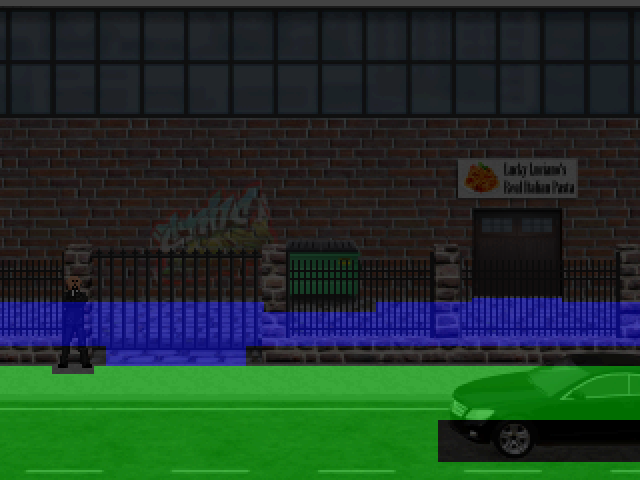
\includegraphics[width=.8\linewidth]{img/walkability.png}
\caption{Walkability bitmap. Source \cite{Shdon}.}
\label{fig:Bitmap}
\end{figure}

However, the user of the framework would most probably need to create this bitmap by themselves. In addition, modifying the bitmap is very difficult and time-consuming. Our aim is to make the experience user-friendly and this solution would go against that. 

The second and arguably more suitable approach enables us to create the map in the Unity Engine itself. To achieve this, the boundaries of the walkable map and obstacles must be defined. A map consisting of polygons offers itself as a solution to this problem, depicted in Figure. The user of the framework would be able to modify the shapes on the fly, making it easy to change the map even late in the development of the game. The idea is to have one primary polygon where characters and other interactable objects are located. Except for that, there are areas that the player cannot currently or indefinitely enter and these can be defined by an arbitrary number of polygons. 


\begin{figure}[H]
\centering
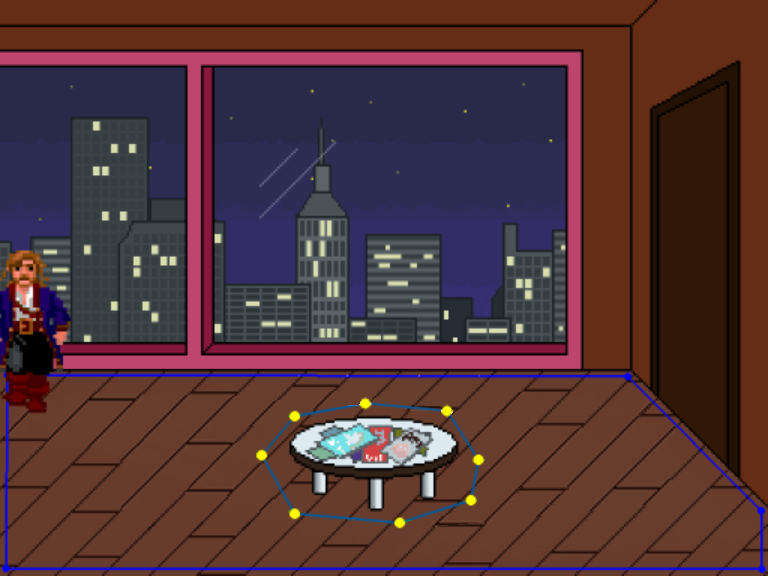
\includegraphics[width=.8\linewidth]{img/WS-polygons2.png}
\caption{Polygonal map. Source \cite{Uurloon1}.}
\label{fig:Bitmap}
\end{figure}

\subsection{Shortest path problem}
Naturally, we don’t want the character to wander aimlessly in search of the endpoint. The problem of finding the shortest path has been extensively researched, with many proven algorithms to solve it. One of the most widely used is the A* algorithm—a graph traversal and pathfinding method known for its efficiency. It is commonly applied in various fields of computer science, including game development, and is described in Algorithm \ref{alg:AStar}. 

\algrenewcommand\algorithmicrequire{\textbf{Input:}}
\algrenewcommand\algorithmicensure{\textbf{Output:}}
\renewcommand{\alglinenumber}[1]{#1.}

\begin{algorithm}
\caption{A* Search Algorithm}\label{alg:AStar}
\begin{algorithmic}[1]
\Require Start node $start$, Goal node $goal$
\Ensure Path from $start$ to $goal$ or failure
\Statex
\Function{A\_Star}{$start, goal$}
    \State $openList \gets \{start\}$
    \State $closedList \gets \emptyset$
    \State $start.g \gets 0$
    \State $start.h \gets \Call{Heuristic}{start, goal}$
    \State $start.f \gets start.g + start.h$
    \State $start.parent \gets null$
    \While{$openList \neq \emptyset$}
        \State $current \gets$ node in $openList$ with lowest $f$ value
        \If{$current = goal$}
            \State \Return \Call{Reconstruct\_Path}{$current$}
        \EndIf
        \State remove $current$ from $openList$
        \State add $current$ to $closedList$
        \For{each $neighbor$ of $current$}
            \If{$neighbor \in closedList$}
                \State \textbf{continue}
            \EndIf
            \State $tentative\_g \gets current.g + \Call{Distance}{current, neighbor}$
            \If{$neighbor \notin openList$}
                \State add $neighbor$ to $openList$
            \ElsIf{$tentative\_g \geq neighbor.g$}
                \State \textbf{continue}
            \EndIf
            \State $neighbor.parent \gets current$
            \State $neighbor.g \gets tentative\_g$
            \State $neighbor.h \gets \Call{Heuristic}{neighbor, goal}$
            \State $neighbor.f \gets neighbor.g + neighbor.h$
        \EndFor
    \EndWhile
    \State \Return failure
\EndFunction
\Statex
\Function{Reconstruct\_Path}{$current$}
    \State $path \gets \emptyset$
    \While{$current \neq null$}
        \State add $current$ to beginning of $path$
        \State $current \gets current.parent$
    \EndWhile
    \State \Return $path$
\EndFunction
\end{algorithmic}
\end{algorithm}

To use the A* algorithm, we first need a graph, so we must define one. A graph is a data structure consisting of nodes and the connections between them are defined by edges. However, in our case, creating a graph with all possible nodes and edges is unnecessary and even impractical—we need to filter out only the relevant information.

A node is included based on the shape and type of the corresponding polygon. In basic shapes like triangles, rectangles and squares, any two points can be connected by a straight line without encountering obstacles. However, if the walkable area is concave (containing one or more nodes with interior angles greater than 180 °), some vertices point inward, creating obstructions that block direct visibility between points, which is depicted in Figure \cite{Polygons}. To account for these obstructions, a node is added to the graph only if its vertex is concave. Convex vertices have an interior angle that is no more than 180 ° and are therefore excluded as they do not create any obstacles. Regarding edges, an edge is included in the graph only if the two nodes that form it are within each other’s line of sight.


\begin{figure}[H]
\centering
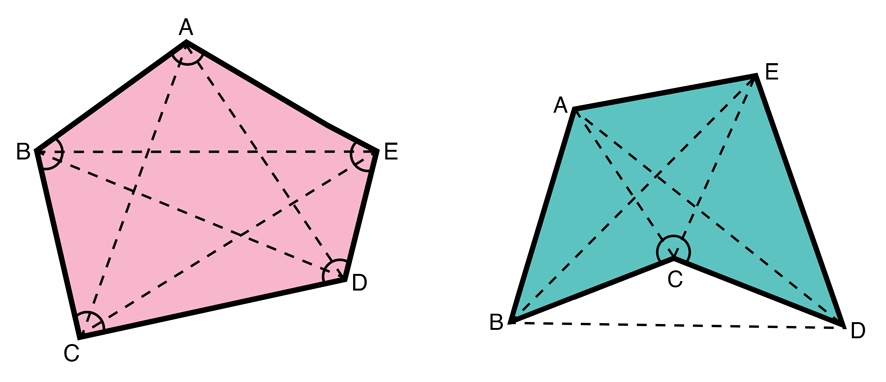
\includegraphics[width=.8\linewidth]{img/polygons.png}
\caption{Convex (left) and concave (right) polygons. Source \cite{Polygons}.}
\label{fig:Polygons}
\end{figure}


The situation is reversed for obstacles (meaning non-main polygons) as we do not want to stay inside these obstacles but on the outside. Since we need to go around them, in this case we take into account convex vertices instead of concave ones. Here, the concave vertices do not stand in the way of two points, but the convex ones do. 

A key component of the A* algorithm is the heuristic function which estimates the cost of the cheapest path to the goal. If the function never overestimates it, A* is guaranteed to return one of the shortest paths from start to goal. Common heuristic functions satisfying this condition include the Manhattan distance and the Euclidean distance. For the purpose of free character movement on a 2D plane, the Euclidean distance was chosen as a heuristic function. It can be calculated from the Cartesian coordinates of the points while also applying the Pythagorean theorem:

\[
d = \sqrt{(x_2 - x_1)^2 + (y_2 - y_1)^2}
\]

\section{Depth Simulation}
As we have specified in Requirements \ref{intro:req:scale} and \ref{intro:req:layers}, we want to simulate the feeling of a 3D space.

by dynamically scaling the character as well as adjusting the layer order of objects.

\subsection{Scaling}
Firstly, we will look closely at character scaling. 

\subsection{Layering}
Next, let us examine the layering. Our aim is to dynamically adjust the visibility of objects, as seen in Figure \ref{fig:Layers}. Because we are working with a 2D space, we have to do a bit more work determining in what order the sprites of objects should be displayed. Fortunately, it is very simple to do since all we need is to look at the Y coordinates. If object A has a smaller Y coordinate than object B, it means that A should be drawn on top of B. 


\begin{figure}[H]
\centering
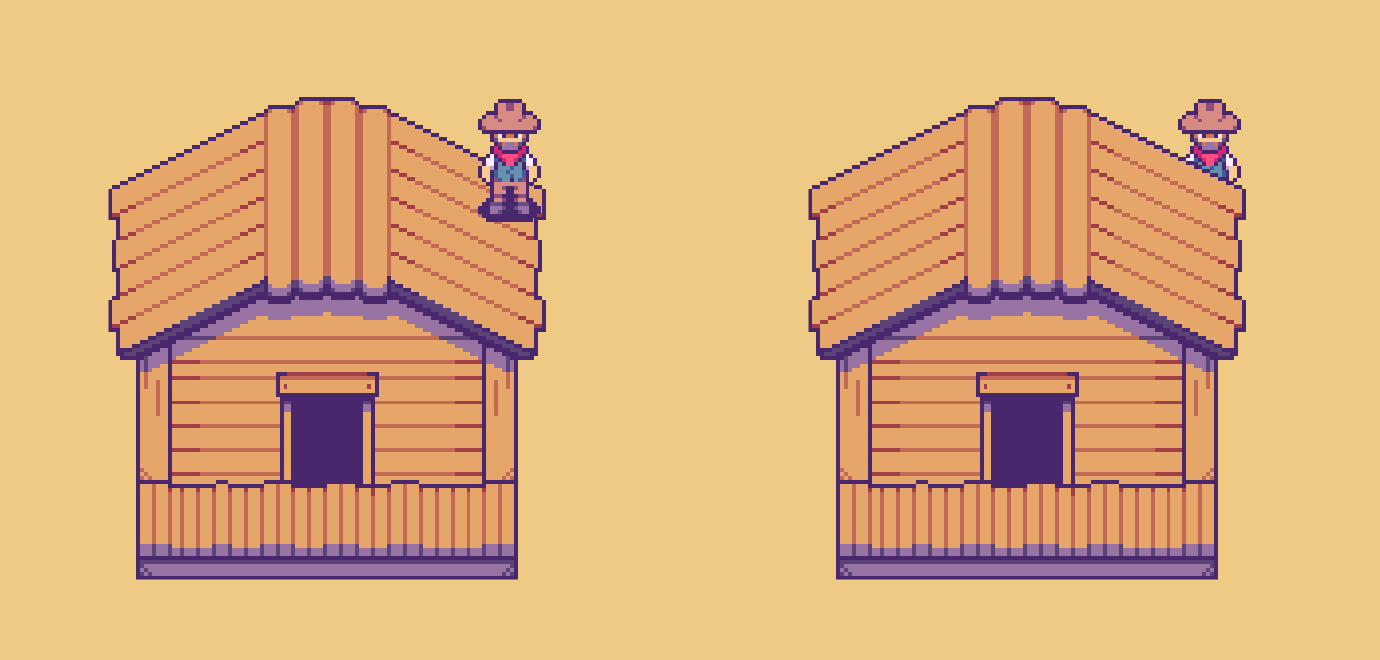
\includegraphics[width=.8\linewidth]{img/layers.png}
\caption{Wrong (left) and correct (right) layer ordering. Source \cite{Piotr}.}
\label{fig:Layers}
\end{figure}

\section{Inventory System}


\section{Dialogue System}



\chapter{Developer Documentation}
This chapter outlines the details of the implementation of the TaleCraft framework along with the overall project structure. Our framework is developed using Unity version 2022.3.61f1 and is compatible with Unity Hub, which can be used to open and manage the project environment. All referenced files are provided in Attachment A for further inspection.

\section{Architecture}
The core of the project is found in the \verb|Assets/TaleCraft| directory. \verb|Assets| is the standard location in Unity for storing scripts, game assets, and other project resources, and the folder \verb|TaleCraft| is our custom folder. The contents are organized into several subfolders and each of them serves a specific purpose, as described in the sections that follow.

\begin{itemize}
    \item \textbf{Runtime}: This folder contains all scripts that are executed during the game’s runtime. The codebase is further organized into five distinct modules: \verb|Core|, \verb|CommandSystem|, \verb|DialogueSystem|, \verb|InventorySystem|, and \verb|WalkingSystem|. Each of these categories contains specific functionality of the framework.
    \item \textbf{Editor}: It includes scripts that extend or customize Unity Editor. These scripts are not executed at runtime. The folder structure within \verb|Editor| mirrors that of the \verb|Runtime| folder.
    \item \textbf{Prefabs}: This folder holds reusable prefab assets utilized throughout the framework.
    \item \textbf{Resources}: It contains various assets required by the framework, such as sprite images and Unity Style Sheets (USS), which define the visual styling of the UI components. 
    \item \textbf{Examples}: The \verb|Examples| folder includes two prototype projects that demonstrate practical applications of the TaleCraft framework. Each prototype features its own scene along with supporting assets, such as custom scripts, prefabs, fonts, and sprites that are specific to those demonstrations. 
\end{itemize}

In the rest of this chapter, we focus on classes located in the \verb|Runtime| and \verb|Editor| folders, as well as the relations between them. In Figure \ref{fig:TaleCraft}, we can see a simple diagram describing the five main groups the classes can be divided into, as well as the connections between them. These groups are the following: 
\begin{itemize}
    \item \textbf{Core} scripts implement key functionalities of the framework, which include Prefab Manager and Input Manager. This system is closely examined in Section \ref{Core}.
    \item The \textbf{Command System} manages the logic behind interactions for items in the inventory as well as those in the in-game world. It is referenced from the Input Manager in the Core group and more information can be found in Section \ref{CommandSystem}.
    \item The scripts in \textbf{Walking System} take care of creating polygons representing the walkable areas (in)accessible to the player as well as the generating of a graph described in Section \ref{Analysis:Graph}. The system also enables movement of characters, which needs to be called from Command System in order to move closer to the required spot upon clicking on it. The Walking System is further examined in Section \ref{Walkingystem}.
    \item  Dialogue scripts in the \textbf{Dialogue System} handle both user-facing and back-end aspects of the dialogue system, such as managing the editing of dialogue graphs through an interactive interface or the saving and loading of graph data. Additionally, some scripts control the runtime logic of the dialogue nodes during gameplay, including tasks such as hiding or revealing specific choice options, triggering events, and displaying the appropriate dialogue text above the corresponding characters. This system is largely separated from other systems except for the reference to variables and conditions from the Command System. We will look closely at the system in Section \ref{DialogueSystem}. 
    \item Finally, the \textbf{Inventory System} is practically completely separated from other systems. This helps the developer choose what type of inventory they want or if they even want one. It can be, however, referenced from through the Unity Inspector. Scripts included in the system are described in more detail in Section \ref{InventorySystem} .
\end{itemize}

\begin{figure}[H]
\centering
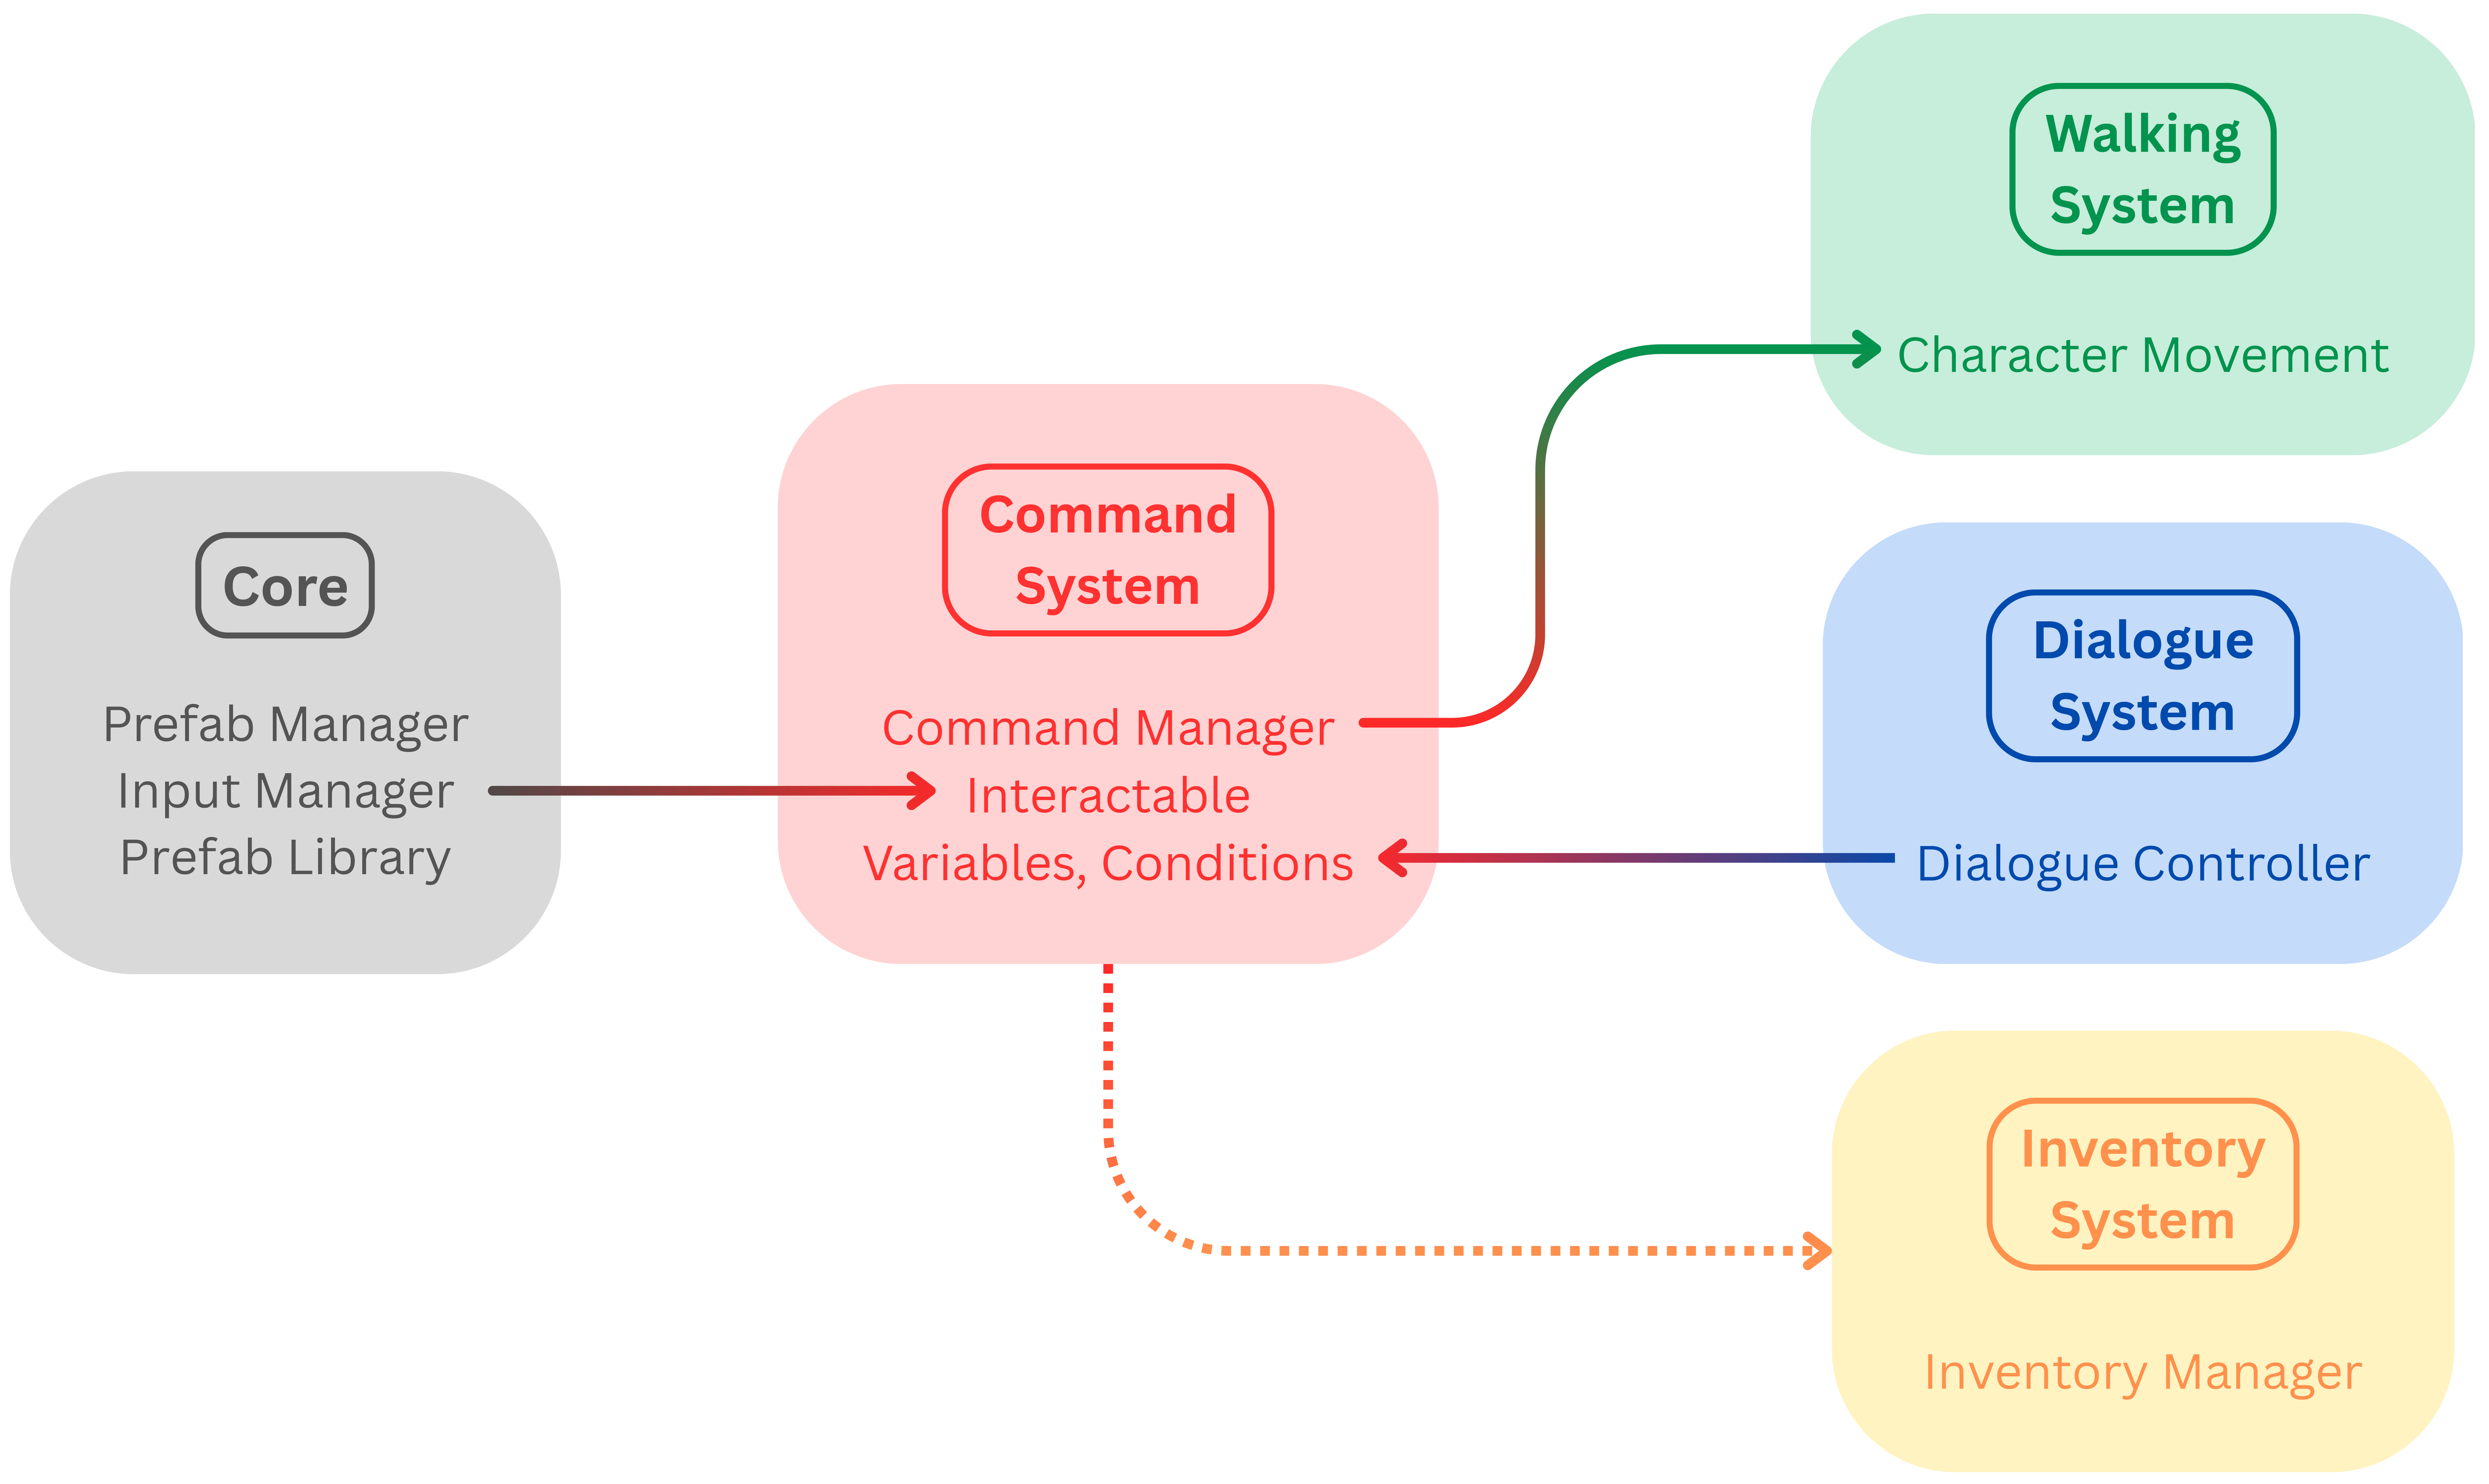
\includegraphics[width=0.85\linewidth]{img/Everything2.png}
\caption{TaleCraft diagram.}
\label{fig:TaleCraft}
\end{figure}

\section{Core}
\label{Core}
The scripts in the Core folder work independently of one another and are responsible for managing foundational functionalities that fall outside the scope of the four main systems. 

\subsection{PrefabManager}
The \verb|PrefabManager| is a singleton that provides global access to shared systems. It holds a reference to the \verb|PrefabLibrary|, which stores prefabs used throughout the game. The singleton instance is created on demand by searching the scene, ensuring only one instance exists by destroying duplicates on \verb|Awake|. For now, it does not include many functionalities, but it can be useful to track gameplay-related logic.

\subsection{PrefabLibrary}
The \verb|PrefabLibrary| is a simple asset manager that stores references to named prefabs, making it easier for other classes to access and spawn them without the need for hardcoded links in the scene or code. It keeps a list of entries, each made up of a name and a corresponding \verb|GameObject|. The main method, \verb|GetPrefabByName|, looks up a prefab by its name and returns the matching object.

\subsection{InputManager}
The \verb|InputManager| class listens for click input. When one occurs, it casts a 2D ray from the mouse position into the world. It also checks each hit collider for a \verb|WorldObject| component and calls its \verb|Interact| method, passing the world position and whether the left or right mouse button is pressed. If no \verb|Interactable| is found, it sends a move command to the player.

\section{Command System}
\label{CommandSystem}
The basis of Command system is built by \verb|CommandManager|, a script whose primary role is to hold commands used in the game. We also need to define objects the player can interact with.  An abstract class appropriately called \verb|Interactable| together with its inherited subclasses \verb|WorldObject| and \verb|InventoryObject| serve that purpose. In order to define suitable actions for each object in the scene, we need to set certain conditions. The classes \verb|Variable| and \verb|Condition| help with that by being able to determine simple logic and comparing variables. There are also two additional scripts that help with setting up the behavior of \verb|InventoryObjects|, namely \verb|TriggerSetter| and \verb|SlotManager|.

\subsection{Variables}
The \verb|Variable| classes define a system of variables, each based on a generic base class. They use \verb|ScriptableObjects|, so variables can be created as assets and shared across the framework. The core is the generic abstract class \verb|Variable<T>|, which stores a \verb|DefaultValue| (set in the inspector) and a \verb|RuntimeValue| (the current value used in the game). When the variable is enabled, it automatically resets \verb|RuntimeValue| to \verb|DefaultValue|. The class also provides methods to set or reset the value. Each concrete subclass specializes this for a specific type:

\begin{itemize}
    \item \textbf{BoolVariable} handles booleans and adds methods to set true, set false, or flip the value.
    \item \textbf{IntVariable} handles integers and adds arithmetic operations like add, subtract, multiply, plus increment and decrement methods.
    \item \textbf{FloatVariable} works like IntVariable but for floats, supporting the same arithmetic and increment/decrement.
    \item \textbf{StringVariable} simply inherits from the generic base and does not add extra functionality since strings typically don't have arithmetic.
\end{itemize}

 \subsection{Conditions}
The \verb|Condition| classes provide a system for defining and evaluating various checks in the framework. At the core is an abstract base \verb|Condition| class that creates the common interface and functionality for all conditions. Building on this foundation, other subclasses handle specific data types such as boolean, integer, float, and string. Each of them compares the current runtime value of a variable with a target value to determine whether the condition is met: 

\begin{itemize}
    \item \textbf{BoolCondition} checks if a boolean variable matches an expected true or false value. It simply compares the variable’s current runtime value with the \verb|ExpectedValue| and returns true if they are equal.
    \item \textbf{IntCondition} checks an integer variable against an expected integer using one of several comparison operators (equal, not equal, greater than, less than, greater or equal, less or equal). The comparison to use is specified by the \verb|Comparison| enum. The \verb|Check| method runs the relevant comparison and returns whether the condition is met.
    \item \textbf{FloatCondition} works similarly to \verb|IntCondition|, but for float variables. It compares the current float value with an expected float using the same set of operators defined by the \verb|Comparison| enum.
    \item \textbf{StringCondition} checks whether a string variable’s current value exactly matches a specified expected string and returns true if they are identical.
\end{itemize}

\subsection{Interactable}
The abstract class \verb|Interactable| serves as the main class for any game object that the player can interact with in the TaleCraft system. It holds a list of \verb|CommandActions| that determine the behavior of the object when certain conditions are met. 

The Figure \ref{fig:Interactable} describes the process of evaluating logic when a click is detected. When the player interacts with the object, the class first registers this interaction in the \verb|CommandManager|’s current sequence, linking the involved \verb|Item| (see \ref{Items}) and \verb|Interactable|. It then looks up the command that matches the currently selected command GUID in the \verb|CommandManager|. Before running the command, it checks whether the interaction sequence matches the command’s sentence structure rules (if those are enabled), which makes sure the player has interacted with the required number of objects. If everything checks out, the command execution includes moving the player closer to the target if the custom action demands it. Then, the class triggers the appropriate Unity Events linked to that command action. If no matching custom action is found, it executes the default action defined by the \verb|CommandManager|.

\begin{figure}[H]
\centering
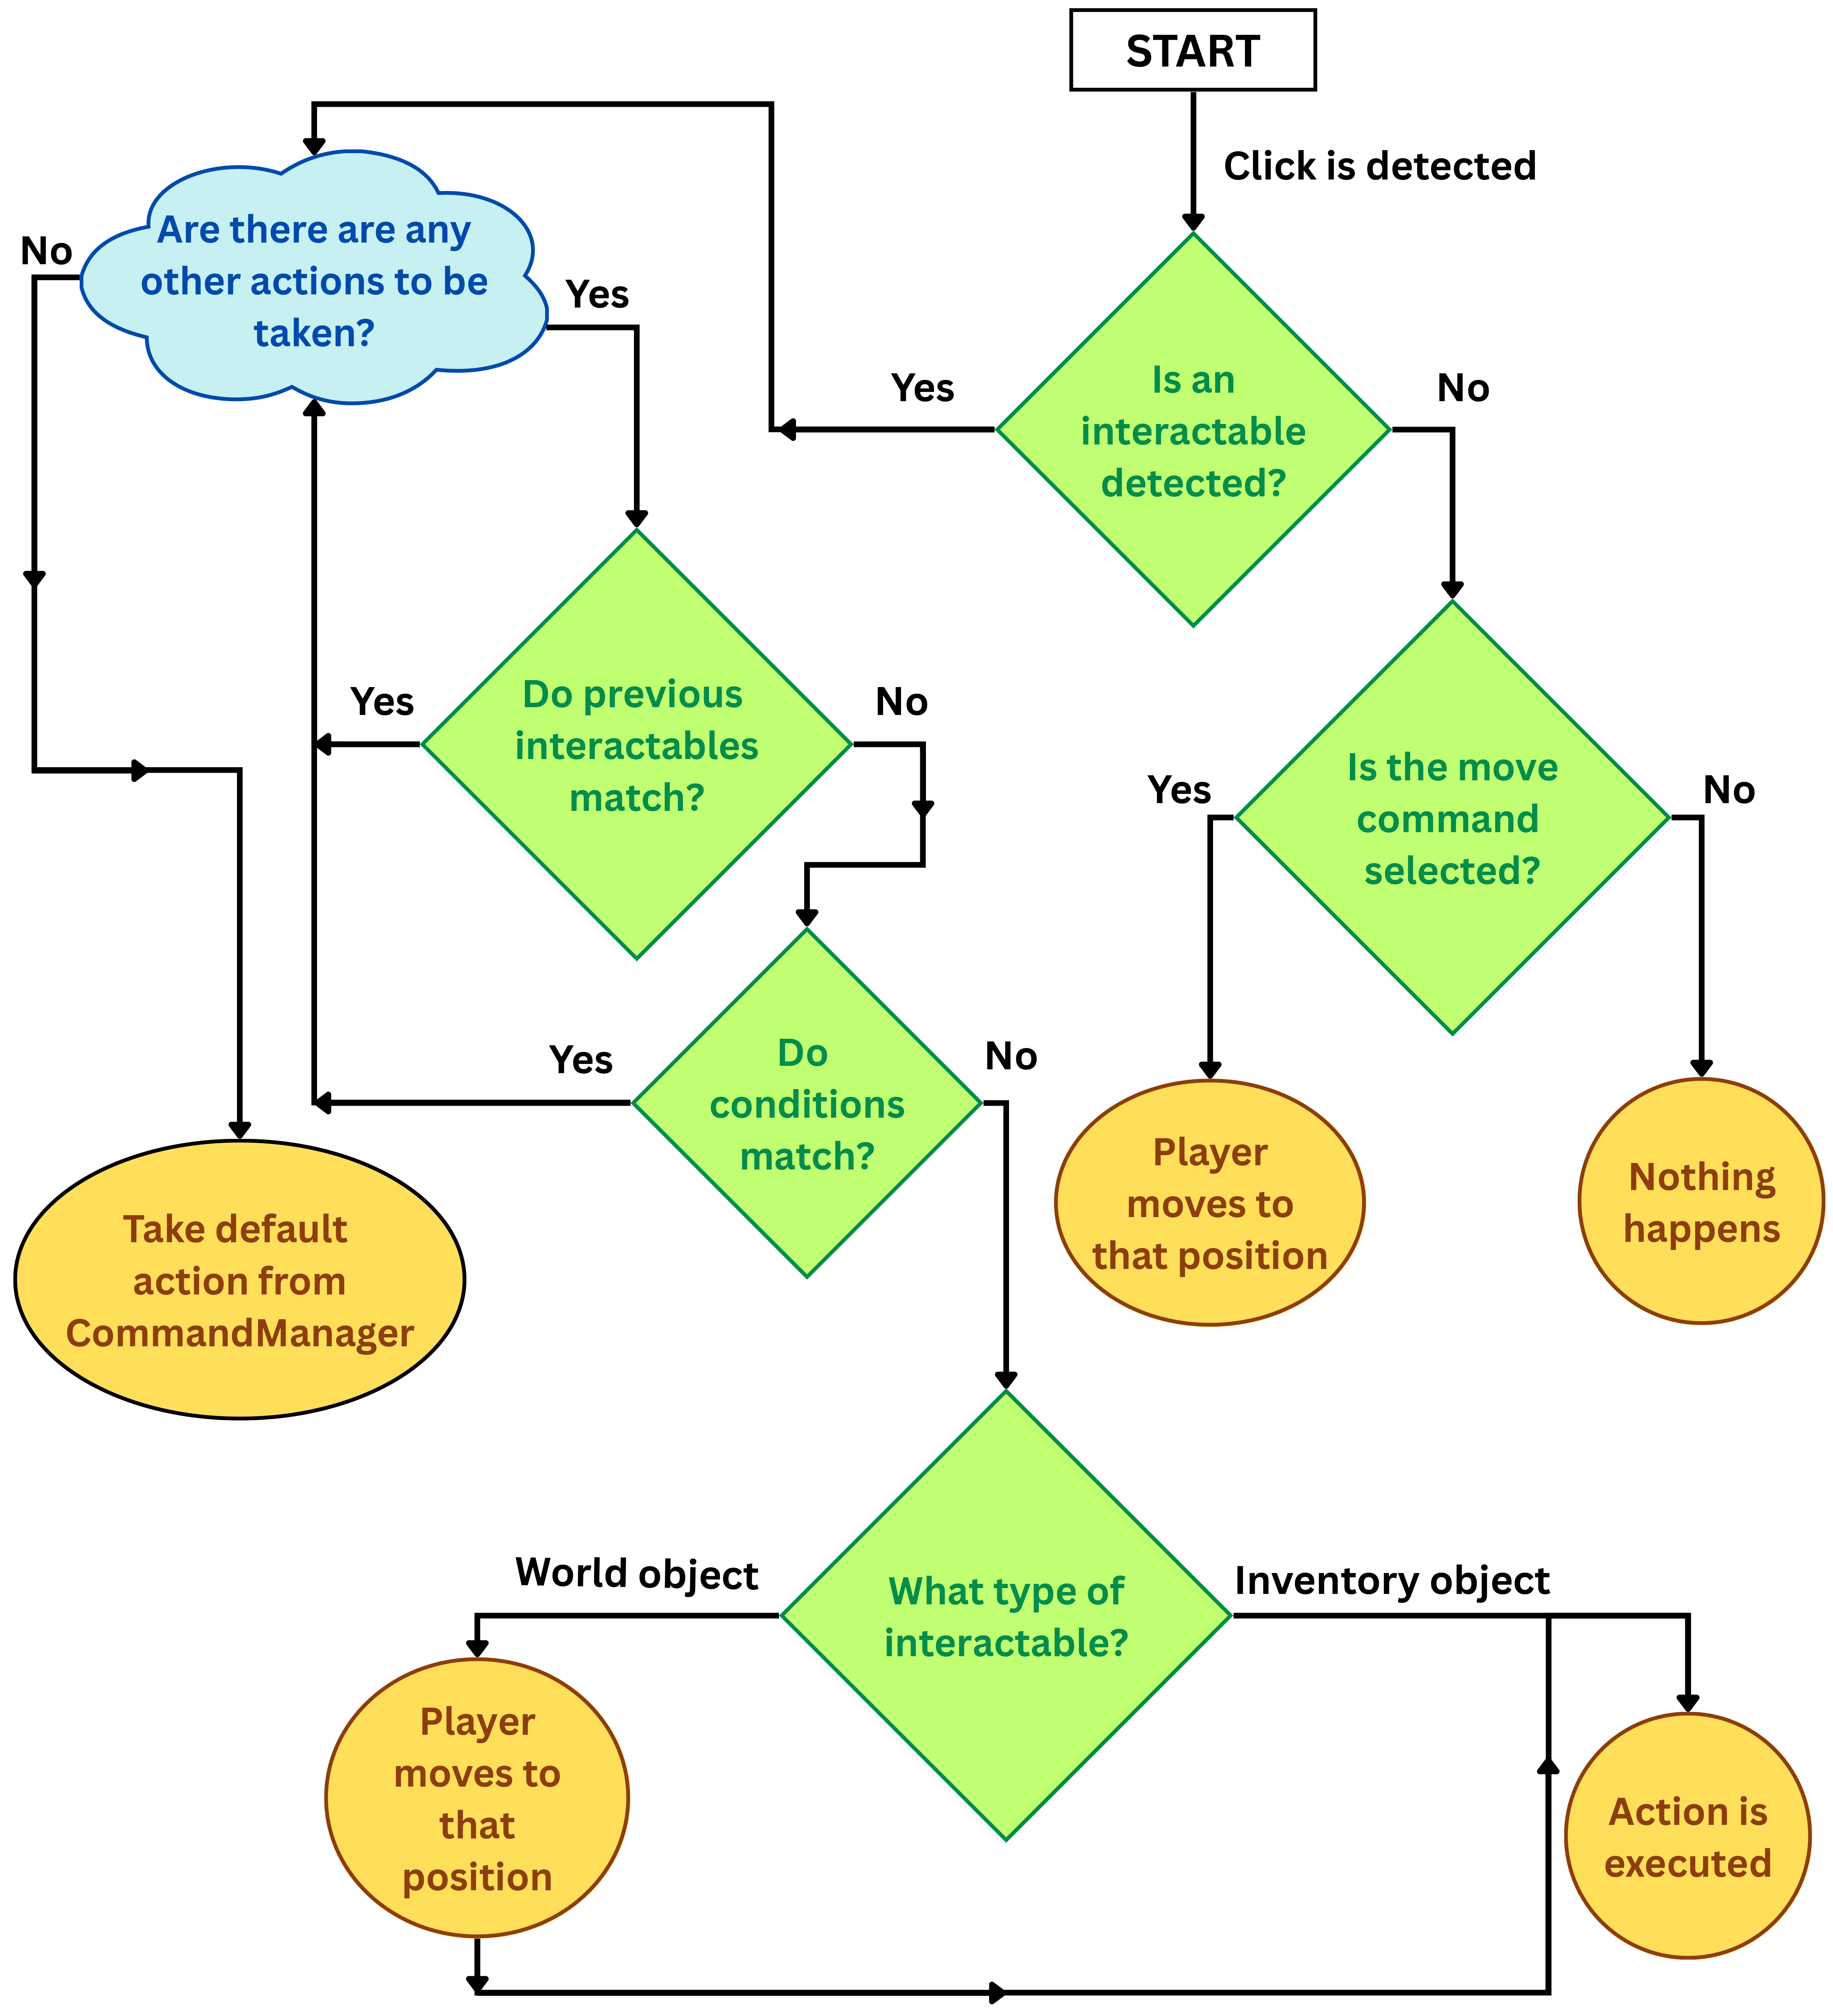
\includegraphics[width=0.9\linewidth]{img/Commands3.png}
\caption{Logic system.}
\label{fig:Interactable}
\end{figure}

\subsubsection{WorldObject}
\verb|WorldObject| extends \verb|Interactable| to represent interactable objects located in the game world, each linked to a \verb|WorldItem|. The class supports an array of \textit{Go-To} points, which are positions the player can move to before interacting with the object. When executing a \textit{Move Closer} command, it calculates the shortest navigable path among these points and directs the player there. If no such point is found, it moves to the clicked position. The class also adds the option to display UI tags when the mouse cursor enters the object.

\subsubsection{InventoryObject}
\verb|InventoryObject| extends \verb|Interactable| to represent items held in the player’s inventory. Unlike other interactables in the game world, it does not work with world objects but instead with inventory slots. It finds command actions specific to the inventory item through the \verb|SlotManager|, which helps to reference items in the scene. 

\subsection{CommandManager}
The \verb|CommandManager| class is a singleton responsible for managing player commands, interaction sequences, and movement logic. It tracks three key commands \verb|selectedCommand|, \verb|defaultCommand|, and \verb|moveCommand|, which are stored as indices referencing a serialized list of \verb|CommandData|. Interaction sequences are stored in \verb|actionSequence|, which logs item-to-object interactions via \verb|ItemInteractablePair|. Temporary interaction data is kept in \verb|ActionTemp|, usually used when a mouse is hovering over an \verb|Interactable| object. The manager also supports basic grammar rules of commands through a list of \verb|SentenceStructure|, which defines valid object-connector sequences. Default actions are stored in \verb|DefaultActions|, a list of \verb|BasicCommandAction| objects that contain a reference to the command, a flag for movement behavior, and a UnityEvent for triggering actions.
 

\subsection{TriggerSetter}
The \verb|TriggerSetter| class manages interactive behavior for inventory. It handles user input like hovering, clicking, and dragging, and links these actions to the appropriate inventory or command responses. Each instance is connected to an \verb|InventoryObject|, which allows it to connect behavior to items in the player's inventory.

On startup, the class loads any required prefabs, such as the drag icon used during item movement, and sets up event listeners from \verb|CommandManager| to reset the UI when a command sequence ends. Mouse clicks on the slot trigger interactions are tied to the currently selected command, while hovering displays item details using shared UI elements to keep the interface clean and consistent. When the player begins dragging an item, a drag icon is created as a copy of the current inventory slot. This icon visually follows the mouse, while raycasts constantly check for valid drop targets underneath, such as another inventory slot or a world object. If the item is dropped on another \verb|Interactable|, the object’s \verb|Interact()| method is called. If no valid target is found, the command is canceled.

\subsection{SlotManager}
The framework must be able to let users define the behavior when inventory items interact with other items. It is not possible to define these actions in the instances of the items themselves, as doing so would be very difficult when crossing to other Unity scenes, since we can only reference \verb|GameObjects| of inventory items he \verb|SlotManager| holds a collection of \verb|Slot| instances, each pairing an \verb|InventoryItem| with its possible command actions.

A \verb|Slot| class links a single inventory item to a list of \verb|CommandActions|, which represent individual commands a player can use with that item. Each \verb|CommandActions| contains a reference to \verb|CommandData| (defining the command’s ID and name) and a list of \verb|LabeledAction|s. These labeled actions wrap a \verb|CustomAction| with a descriptive label, which link an action to a meaningful human-readable name.

\verb|CustomAction| holds the execution details for a command: it can require \verb|Interactables|, track previous ones, and check custom conditions before running. It also manages separate UnityEvents for left and right mouse clicks, with options to move the player closer during the interaction and duplicate actions across click types.


\subsection{Action Drawer and Window}
To organize the commands, we use the classes \verb|LabeledActionListDrawer| and \verb|ActionEditorWindow|. The \verb|LabeledActionListDrawer| is a utility designed to make it easier to manage a list of \verb|LabeledActions| directly in the Inspector. The \verb|Initialize()| method sets up \verb|ReorderableList|, including custom drawing behavior for each item. Each entry in the list includes an option to open a separate \verb|ActionEditorWindow| for modifying the action’s configuration. This class is a custom Unity \verb|EditorWindow| designed to provide a user-friendly interface for editing \verb|LabeledAction| objects in Inspector. When launched via the static \verb|Open()| method, the window shows collapsible sections for different components of the action. These include a list of \textit{Previous Interactables} (other objects this action may rely on), a list of editable \textit{Conditions}, and settings for mouse button triggers.

The \textit{Previous Interactables} list contains all \verb|Interactables| that are required to have been interacted with in order to execute this action. \textit{Conditions} can be added dynamically using a context menu that finds all non-abstract subclasses of \verb|Condition| via reflection. Finally, the window allows editing separate action lists for left and right mouse buttons. If the \verb|DuplicateActions| option is enabled, however, the editor shows a shared list of actions for both mouse clicks. 

\subsection{DisplayCommands}
The \verb|DisplayCommands| class is responsible for managing the visual layout and behavior of command buttons in the Unity UI. It keeps track of the currently active commands and also stores any commands from the global \verb|CommandManager| that are not currently shown. 

On startup, it sets up the buttons by assigning each one a name and hooking up a click listener that selects the corresponding command using its GUID. The button labels are set through the \verb|ApplyCommandNames()| method, which looks up the name of the linked \verb|CommandData|. The \verb|ReloadUnused()| method checks for commands that exist globally but are not in the current UI and stores them separately for possible future use. To keep the interface clean, \verb|RemoveChildren()| deletes buttons that no longer match a valid command. If the command name changes, \verb|ReloadUIName()| updates the button label. Button clicks are set through \verb|SetClick()|, which connects each button to the global command selection logic. Finally, \verb|GetPosition()| calculates the placement of each button on the grid based on layout parameters such as spacing, column count, and offset.

 \subsection{DisplaySentence}
In Section \ref{ActionPanel}, we decided to implement a sentence that indicates the current sequence of actions for the player. The \verb|DisplaySentence| class handles rendering a sentence in the UI and updates dynamically based on the currently selected command and its sentence structure (defined in \verb|CommandManager|). During each frame, it checks if the text component is valid and updates its content using the \verb|GetSentence()| method. If \verb|onMouse| is enabled, the sentence display is also repositioned to follow the mouse, offset by the \verb|shiftBy| value.

The sentence is built using the \verb|SentenceStructure()| of the selected command. It always begins with the command’s base name and then adds other elements according to a list of rules. These rules define whether each part of the sentence should be a connector (like a keyword) or an object (like an item or interactable).

If a rule calls for a connector and one is available, it is inserted into the sentence. If it expects an object and one is present in the current \verb|ActionSequence|, it uses the object's name. If no object is available, but there is a temporary action, it uses that instead and stops the sentence there.


\section{Walking System}
\label{Walkingystem}
The core component of the walking system (illustrated in Figure \ref{fig:WalkingSys}) is the \verb|WalkingMap| class. The project provides a prefab that includes a \verb|GameObject| with the \verb|WalkingMap| script attached as a component. This prefab also contains a child \verb|GameObject| with a \verb|Polygon| component that defines the walkable area in the game scene. The \verb|WalkingMap| is responsible for managing a collection of polygons, each representing regions where characters are allowed to move. An instance of this prefab can be automatically instantiated into the scene hierarchy through a custom menu option, using the \verb|WalkingSystem| class. The next important part of the system is class \verb|PathFinder|, which determines how a character should navigate from one point to another by calculating the paths through a graph structure. The graph is represented by class \verb|Graph|, which consists of \verb|GraphNodes| and \verb|GraphEdges| that are set based on the geometry of the walkable area. The class \verb|CharacterMovement| then uses the paths created by \verb|PathFinder| to move characters around the scene. Finally, \verb|SpriteScaler| dynamically adjusts the visual scale of the character based on the position on the map, giving the illusion of depth. Together, these components form the complete walking system used in TaleCraft.


\begin{figure}[H]
\centering
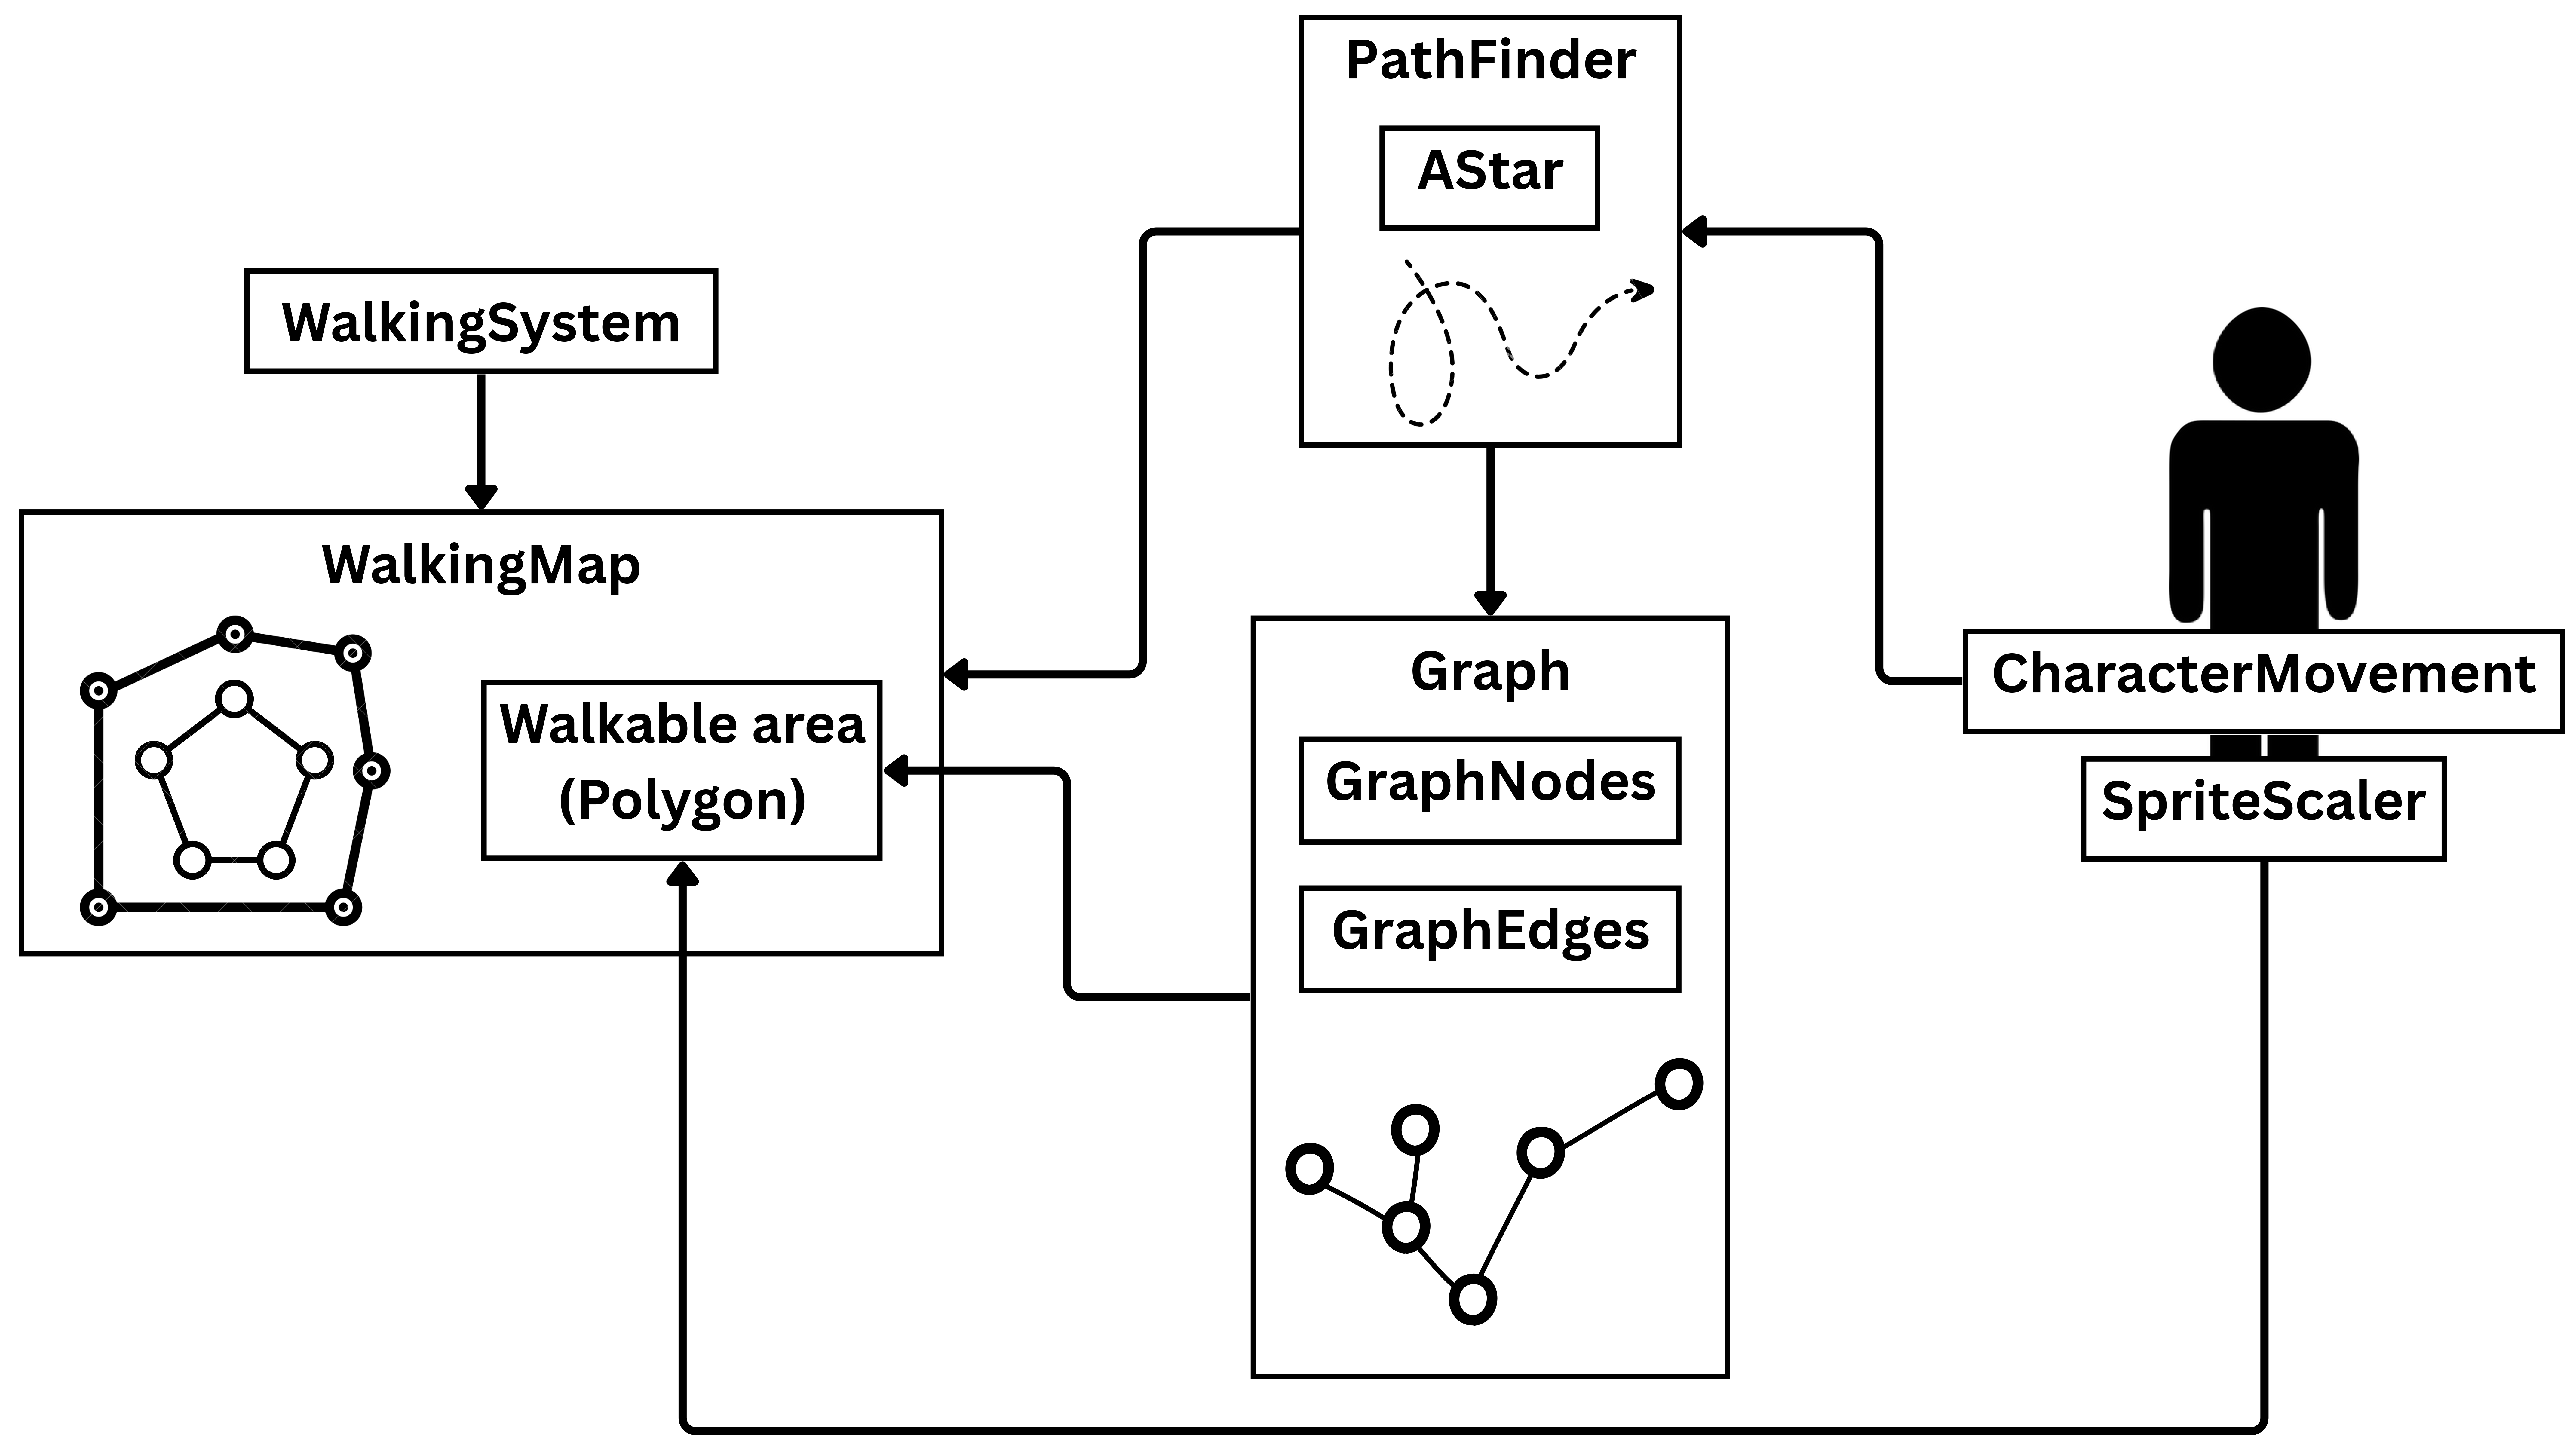
\includegraphics[width=0.85\linewidth]{img/Walking2.png}
\caption{Walking system.}
\label{fig:WalkingSys}
\end{figure}

 
\subsection{Polygon}
In Section \ref{Analysis:Polygon}, we decided to represent the walkable area as well as the obstacles in form of polygons, so let us have a look at its implementation. The \verb|Polygon| class defines a collection of connected points (\verb|GraphNode|s) that form a polygon in a 2D space. It is designed to run both during gameplay and in the Unity Editor, where it dynamically manages and visualizes its vertices using Gizmos. The class ensures that the vertices are ordered clockwise for correct algorithmic behavior, which is validated by the \verb|IsOrientationClockwise()| method.

To assist in pathfinding and calculations, \verb|Polygon| includes methods to determine whether a point lies inside the shape, whether a point should be removed from the polygon, and where the nearest point on the polygon's edge is relative to a given location. These checks are based on geometrical principles such as ray-casting and distance-to-segment calculations. In edit mode, the polygon continuously scans its child objects to update its list of vertices using the \verb|ListChildrenWithComponent()| method. It expects these children to have a \verb|Point| component and uses their positions to form the polygon.

Graphical properties like edge drawing, point visibility, and point scaling are configurable and updated automatically. The editor visualization adapts to zoom using Unity’s handle size system to keep consistent point sizes when viewing in the Scene window.


\subsection{Graph}
\verb|Graph| class represents a cyclic, undirected graph composed of \verb|GraphNode| vertices and \verb|GraphEdge| connections. It is the foundational data structure used in pathfinding, as established in Section \ref{Analysis:Graph}. Each node is stored in a list, and its neighbors are tracked in a parallel adjacency list. Edges between nodes are recorded in a dictionary, keyed by the smaller of the two node indices, which ensures that the edges do not repeat.

The graph provides utility functions for calculating Euclidean distances between nodes and between a point and a line segment, which are essential for visibility checks and path optimization. Nodes and edges can be dynamically added. When an edge is added, it is also registered in the neighbor lists of both nodes to maintain symmetry. The graph keeps references to a \verb|Start| and \verb|End| node, which are required for executing the pathfinding algorithm.

 A \verb|GraphNode| encapsulates a 2D coordinate and an optional reference to a \verb|Point| game object. It serves as a vertex in the \verb|Graph|. Nodes can be constructed from Unity \verb|Vector3|, raw coordinates, or \verb|Point| objects. The node exposes its position through \verb|X|, \verb|Y|, and a \verb|GetLocation()| method that returns a \verb|Vector2|.

 A \verb|GraphEdge| represents an undirected connection between two graph nodes, identified by their indices and storing a precomputed length for efficiency. The edges are normalized so that the smaller node index is always \verb|N1|, which makes storage and retrieval in \verb|Graph| easier.


\subsection{PathFinder}
\verb|PathFinder| is responsible for calculating the shortest navigable route between two points inside the walkable area defined by \verb|WalkableMap|. It constructs a visibility graph based on polygonal data and uses A* search to determine the optimal path.

The core logic starts by constructing a graph in which nodes are placed at concave vertices of the defined walkable area and obstacle polygons. Additional nodes are inserted at the given start and end positions, which can be adjusted to meet constraints, such as staying inside the main polygon or outside obstacles, depending on the settings of \verb|WalkableMap|.

To determine possible connections between nodes, \verb|PathFinder| uses line-of-sight (LOS) checks. These ensure that no segment intersects any polygon edge and that the midpoint of each connection lies in the walkable region and outside obstacles. Nodes that satisfy the LOS criteria are connected with graph edges. The shortest path is then computed using an A* algorithm in the \verb|AStar| class, which uses a Euclidean heuristic function.  The resulting path consists of a list of \verb|GraphNode| points and their respective distances. For visualization purposes, the class can draw both the full graph and the shortest path using Unity Gizmos.



\subsection{SpriteScaler}
In order to simulate depth and give characters the appearance of existing in 3D space (as discussed in Section \ref{analysis:depth:scaling}), the \verb|SpriteScaler| class dynamically adjusts the scale of a \verb|GameObject| based on its position.  The scale is continuously updated during both runtime and edit mode using the \verb|[ExecuteAlways]| attribute. This makes the object's size always match its intended perspective in the scene. Having the correct scale during editing is especially useful when setting up the layout before running the game. The class supports multiple scaling modes including none, X-axis-based, Y-axis-based, and a custom scale blending based on proximity to vertices of a defined polygonal walkable area.

Using configurable parameters such as \verb|upperScale|, \verb|lowerScale|, and \verb|perspectiveFactor|, the first two modes (X-axis / Y-axis scaling)  calculate the appropriate scale by interpolating the object's position relative to the walkable polygon’s bounds. The custom scaling mode, on the other hand, employs a weighted average of vertex scales that is inversely proportional to their distance. 


\subsection{CharacterMovement}
The \verb|CharacterMovement| class manages the movement itself. It holds a reference to a \verb|WalkableMap| and a pathfinding system (\verb|PathFinder|) in order to compute traversable paths between points. Movement allows the character to smoothly interpolate along a computed path using coroutines while adapting the speed based on the object's scale via the \verb|SpriteScaler| component. The \verb|Move| methods handle both direct target positions and precomputed paths, initiating a coroutine that interpolates the character’s position over time. The class also ensures that if a new movement command is issued mid-transition, the current motion is canceled, and a new path is created. It also supports visual debugging via Unity’s Gizmos for path visualization.

 
\subsection{WalkableMap}
Everything comes together in \verb|WalkableMap|, which manages the pathfinding logic in a scene by maintaining and organizing the walkable area and a collection of obstacles. It is responsible for ensuring that the start and end points of a path remain within valid constraints, such as staying inside the main walkable polygon or outside defined obstacles.

The class is initialized by identifying all child objects tagged as obstacles and storing their corresponding \verb|Polygon| components. These obstacle polygons, along with the main walkable polygon, are used to construct a map for navigation. Any null references inside the obstacle list are actively removed to maintain consistency. \verb|WalkableMap| also provides options to visualize the graph's structure and the calculated path in the editor using specified colors from the inspector.

\subsection{WalkingSystem}
The \verb|WalkingSystem| class provides editor functionality to instantiate a predefined walking system prefab into the current Unity scene. It integrates into the Unity Editor menu and allows developers to quickly add the walking system via a custom menu item. After clicking on the option, the class finds the corresponding prefab from a centralized \verb|PrefabLibrary|, and instantiates it in the hierarchy.


\section{Inventory System}
\label{InventorySystem}
Inventory system consists of three main components: a way to represent items in the framework (the \verb|Item| class, discussed in Section \ref{Items}); a manager that keeps track of the inventory’s contents (\verb|InventoryManager|, detailed in Section \ref{InventoryManager}), and a UI component that visually displays the inventory (\verb|DisplayInventory|, covered in Section \ref{DisplayInventory}). 

\subsection{Items}
\label{Items}
The \verb|Item| class and its subclasses define the different item types used in TaleCraft’s inventory system. They take advantage of Unity’s \verb|ScriptableObject| to make managing and saving item data easier.

At the base is the \verb|Item| class, which stores basic information, such as the item’s name and description. It also includes a simple method to rename the item when needed.

The \verb|InventoryItem| class inherits from \verb|Item| and adds data for how the item should appear in the UI. This includes an \verb|ItemImage| that holds a sprite and a color. The \verb|ApplyTo()| method lets us apply this image data to a Unity UI Image component, ensuring that the item is displayed correctly in the inventory. \verb|ItemImage| is a straightforward container for the sprite.

Lastly, \verb|WorldItem| is another subclass of \verb|Item| meant for items that exist in the game world but might not be carried by the player. It does not add extra features but serves to clearly separate world objects from inventory items for game logic purposes.
 
\subsection{InventoryManager}
\label{InventoryManager}
The \verb|InventoryManager| class provides a basic inventory system using a list to keep track of a collection of \verb|InventoryItem| objects. It also supports adding new items, removing existing ones, and clearing everything from the inventory. Whenever the inventory changes, it executes an event to let any connected systems know about the update. The \verb|RestrictSize| flag determines whether the inventory should enforce a size limit, which is set by the \verb|MaxSize| value.

When adding an item, the manager first checks two things: whether the inventory has reached its size limit (if the size restriction option is turned on), and whether the item is already in the list. If both checks pass, the item is added and the change event is triggered. Removing an item simply tries to take it out of the list. If the item was found and successfully removed, the event is triggered to reflect the update. The \verb|ClearInventory()| method just empties the list completely and notifies any listeners that the inventory has changed.

\subsection{DisplayInventory}
\label{DisplayInventory}
When it comes to displaying the inventory to the player through the UI, the class \verb|DisplayInventory| is responsible for it. It works together with the \verb|InventoryManager| to stay in sync with the actual inventory data and updates the visual elements whenever changes occur. At the beginning, it configures things like slot size, scaling, and layout logic. During initialization, it also looks for a child \verb|GameObject| named \verb|"Items"|. If it does not exist, the class creates it to serve as the container for all item slots. Right after that, it triggers a UI refresh to display the current inventory.

To update the UI, the class either clears or reuses existing slot \verb|GameObjects| to match the number of items in the inventory. For each item, it reuses a slot if one is available, or instantiates a new one from a prefab. Then it fills in the visual content of the slot with the data of the item.

The class supports two display modes: one that shows only the item's icon and one that shows only its name. In both cases, items are arranged using a grid system that calculates each slot’s position based on its index and the total number of columns. To manage larger inventories, only a portion of the items are visible at a time, limited by \verb|MaxItemCount| and controlled using the \verb|ItemIdx| offset. Any items outside this visible range are hidden, and the grid layout is recalculated every time something in the inventory changes.
 
\subsubsection{InventoryScrollButton}
\verb|InventoryScrollButton| manages a scroll button in the inventory UI, allowing users to navigate through a list of items. Depending on its configuration, the button shifts the inventory either forward or backward and updates the item display accordingly. During initialization, the component saves the button's default image color for later use in visual feedback. When the component is enabled or disabled, it subscribes or unsubscribes from inventory change events to ensure the button stays visually consistent with the current inventory state.

The \verb|SetColor()| method updates the button appearance based on whether scrolling is currently possible. If the inventory has reached the beginning or end, the button is visually dimmed using a predefined inactive color to indicate that further scrolling in that direction is not available. When clicked, the \verb|Scroll()| method modifies the \verb|ItemIdx| value that defines the starting index of visible items in the inventory. It then iterates through the inventory’s UI elements, updating their visibility and position so that only the currently relevant items are shown.


\section{Dialogue System}
\label{DialogueSystem}
The centerpiece of the visualization of graphs in the Dialogue system is class \verb|DialogueGraphView| (\ref{devlog:DialogueGraphView}), which uses the main features of the \verb|GraphView| API and displays them using \verb|DialogueWindowEditor| (\ref{devlog:DialogueWindowEditor}). The window then uses elements (\ref{devlog:Elements}) from the API such as nodes, edges and groups to represent a dialogue graph. This is, however, only done through Unity Editor, which means that we cannot access the data during runtime. To solve this, we define \verb|DialogueGraphData| (\ref{devlog:DialogueGraphData}), which stores the values of the elements of the graph together with the relationships between these elements. The final piece of the graph management is a saving and loading system intuitively called \verb|DialogueSaveLoad| (\ref{devlog:DialogueSaveLoad}), which serves as a bridge between \verb|DialogueGraphData| and the actual graph in \verb|DialogueWindowEditor|. Now, we are left with \verb|DialogueController| and \verb|DialogueUIController| (\ref{devlog:DialogueController}, \ref{devlog:Dialogue UI}), which manage the logic of traversing the data nodes of \verb|DialogueGraphData| followed by displaying the appropriate UI on the screen. In the following sections, we examine the actual implementations of these classes.

\subsection{Elements}
\label{devlog:Elements}
A graph consists of nodes, edges, and, in our case, also groups (see Section \ref{Analysis:Dialogue:Features}). While Unity’s \verb|GraphView| API provides built-in support for these elements, their default implementations are too minimal for our needs. To support features like saving, loading, and conditional branching, we must extend these base components with additional properties. One such property is a globally unique identifier (GUID), which allows us to keep references to nodes and groups across editing and serialization. In this framework, each node and group is assigned a GUID to support consistent tracking. Edges are defined by the connections between nodes and this relationship can be stored directly in the nodes themselves. Therefore, the following section will closely examine the extended implementations of nodes and groups.


\subsubsection{Nodes}
The nodes are a central piece of the dialogue graph. It consists of various types of nodes.

At the heart of this system is \verb|BaseNode|, which inherits from the \verb|Node| in \verb|GraphView| API and provides all shared behavior for node-based interaction. It handles input/output port creation, holds a unique identifier, and manages condition logic such as booleans, integers, floats, and strings. These conditions are used to control the flow of the dialogue graph based on variables, and the node provides a dynamic UI to configure them. It manages a \textit{Visited} flag, which can be toggled or generated as a \verb|Variable|. All of the other nodes inherit from the \verb|BaseNode| all of the properties as well as the methods.

\verb|StartNode| represents the entry point of a dialogue flow. It is a minimal extension of \verb|BaseNode| and contains a single output port and simple setup for ID and \textit{Visited} state. This node effectively serves as the beginning of the conversation graph, initiating the traversal through the dialogue nodes.

The \verb|DialogueNode|, on the other hand, represents a standard dialogue step in the graph. It contains one input port and multiple output ports for branching conversations, that can only be connected to a \verb|ChoiceNode|. Internally, it holds a list of text boxes where each entry can represent a character's line. It supports two dialogue continuation styles: automatic after a wait time, or manual via player input. The visual elements dynamically adjust based on the continuation type and presence of choice ports. Choices are represented by additional output ports and are stored in \verb|DialogueNodePort| instances.

 The \verb|ChoiceNode| is designed for player decision points. It displays a single text field and conditions that determine whether it appears or not. The node includes one input port and one output port. All conditions are inherited from the base node system and are managed using the overridden methods \verb|AddCondition|.

\verb|BranchNode| extends \verb|BaseNode| to implement decision-making logic. It sets up one input port and two output ports labeled \textit{True} and \textit{False}, allowing the dialogue to split based on the evaluation of its conditions. 

Using \verb|EventScriptableObject|, the \verb|EventNode| allows triggering events assets. These objects reference \verb|DialogueEvent| assets that encapsulate game-side logic. Each event is shown in the UI as an \verb|ObjectField| and can be added or removed with the corresponding buttons. All event assets are stored in a list and serialized through the node class.

Finally, \verb|EndNode| signals the end of a dialogue path. It contains only one multi-input port and no output ports. Internally, it uses an \verb|EnumField| to define how the dialogue ends (exit, return to the start, or repeat the last node). 
 

\subsubsection{Groups}
As established in Section \ref{Analysis:Dialogue:Features}, we would like to have the ability to organize subsets of nodes in the graph, and the \verb|BaseGroup| class serves that purpose. It is an extension of Unity’s \verb|Group| from the \verb|GraphView| system, used in the Unity Editor for grouping nodes visually in a graph interface. It adds a single field, \verb|GroupGuid|, which uniquely identifies the group via a generated GUID. This is useful for saving, loading, and tracking groups independently of their visual layout.


\subsection{DialogueGraphData}
\label{devlog:DialogueGraphData}
In order to access dialogue graphs during the gameplay, we, of course, need a way to represent the data. The \verb|DialogueGraphData| class functions as a data container for the dialogue system. Implemented as a \verb|ScriptableObject|, it exists as a an asset that can be saved, edited, and reused directly in the Unity Editor. Its primary responsibility is to store the entire structure of a dialogue graph, including dialogue lines, choices, branching logic, events, and the connections between nodes.

All node data inherit from the \verb|BaseNodeData| class, which provides common properties such as a unique identifier (GUID), editor position, display name, a runtime \verb|Visited| flag, and a collection of conditions. More specialized node types include \verb|DialogueNodeData| (storing character-linked dialogue text), \verb|ChoiceNodeData| (for player-selectable options), \verb|EventNodeData| (triggering scripted actions), \verb|BranchNodeData| (evaluating conditions), and \verb|EndNodeData| (defining how the dialogue branch concludes).

In addition to node data, the class stores group and edge information. \verb|GroupData| allows developers to visually organize related nodes in the editor by assigning them to named movable containers. Each group includes an ID, a name, a position in the graph view, and a list of GUIDs corresponding to the nodes it contains. \verb|EdgeData| defines the directional links between nodes and represents the logical flow of the conversation. Each edge stores the GUIDs and port names of both the source and target nodes, allowing the system to determine the next node in the sequence during both editing and runtime.


\subsection{DialogueSaveLoad}
\label{devlog:DialogueSaveLoad}
The saving and loading of a graph occurs in the \verb|DialogueSaveLoad| class. It is achieved by serializing and deserializing the data the graphs consist of. When saving, the class converts the current graph state into an asset \verb|DialogueGraphData|. This process involves saving the structure and properties of groups (name, position, and contained nodes), serializing connections between nodes, and storing the data specific to each node type. For example, \verb|Dialogue Nodes| store text box content and port configurations, \verb|Event Nodes| keep references to \verb|ScriptableObject| instances, and \verb|Branch Nodes| save conditional data as well as the GUIDs of the nodes connected to their \textit{True} and \textit{False} outputs.

During loading, the class first clears the current graph to ensure a clean state. Then it reconstructs groups based on the stored data, followed by instantiating nodes using their saved attributes such as position, GUID, \textit{Visited} status, and type-specific data. The nodes are then reassigned to their appropriate groups, and the edges are reconnected by matching saved port names with the correct input and output ports.


\subsection{DialogueGraphView}
\label{devlog:DialogueGraphView}
\verb|DialogueGraphView| inherits from Unity's \verb|Experimental.GraphView| and manages the visual interface and logic of a node-based dialogue system. It supports creation, manipulation, serialization, and deserialization of various dialogue nodes and groups inside the editor. The class also enables standard manipulations such as dragging, selection, and zooming and includes a customizable minimap for navigation. Users can interact with the graph by adding nodes via a search window, grouping them, or copying/pasting selected elements. 

For copy-paste functionality, the class serializes selected nodes, edges, and groups into a \verb|CopyData| class, which regenerates them at the mouse position after pasting. During serialization, each node gets a new GUID and edges are reconstructed by mapping these new GUIDs. The grouping is preserved by reassigning nodes into their respective regenerated groups.

 
\subsection{DialogueWindowEditor}
\label{devlog:DialogueWindowEditor}
The \verb|DialogueWindowEditor| class is a custom Unity Editor window that is used to create and edit dialogue graphs. It is built using Unity’s \verb|UI Toolkit| and works directly with \verb|DialogueGraphData| assets. When one of these assets is opened in the Unity Editor, the \verb|[OnOpenAsset]| callback opens this custom window and loads the selected asset. When the window is enabled, the \verb|OnEnable()| method sets up the main interface. It creates a resizable \verb|DialogueGraphView| that fills the editor panel and adds a toolbar with useful buttons. These buttons let the user save the current graph, load data from the asset, and show or hide the minimap.

\verb|DialogueSaveLoad| then handles saving and loading of graph data, which keeps the file management logic separate from the user interface. When the window is closed or disabled using \verb|OnDisable()|, all visual elements are removed from the UI to prevent memory or display issues.


\subsection{DialogueController}
\label{devlog:DialogueController}
The \verb|DialogueController| class is a central piece that manages the flow of a dialogue that runs during the gameplay. It works with \verb|DialogueUIController| to show or hide dialogue UI elements and displays the content to the player. When a dialogue is started via the \verb|StartDialogue| method, it initializes the system using the provided \verb|DialogueGraphData|, invokes any start events, and immediately begins processing the dialogue from the designated start node.

Through the \verb|CheckNodeType| method, the class handles different node types dynamically, which routes execution to specific functions based on whether the node is a start node, dialogue node, event node, branch node, or an end node. For each node, it sets a \textit{Visited} flag, which can be used to track player progress or avoid repeating dialogue unnecessarily. The dialogue progression is asynchronous: if a node requires player input, buttons are shown, if it should continue automatically, the system waits before continuing to another node.

\subsection{Dialogue UI}
\label{devlog:Dialogue UI}
On the other hand, \verb|DialogueUIController| manages the visual and interactive elements. Its main job is to show dialogue text and player choices during conversations, as well as to handle input like button clicks or key presses to move dialogue forward. It controls visibility of the UI, sets up text boxes dynamically based on who is speaking and where they are in the scene, and adjusts button states depending on the dialogue logic (like whether a choice should be interactable, grayed out, or hidden). Internally, the class caches and stores UI elements like buttons and text boxes to reuse them efficiently across dialogue sequences. It also supports positioning UI elements relative to characters in the game world, so that text appears near the speaker.
\chapter{User documentation}
In the first part, this chapter introduces a description of the framework itself with all its features. The second part then provides a description of the two showcase games with the way they are controlled.  

\section{Framework}
The TaleCraft framework consists of five main systems whose role is to manage and execute the primary features of a point-and-click adventure game. We will go through them and explain the ideal process of creating a game using this framework. The project also includes two scenes showcasing the use of our framework. In this chapter, we will refer to these two scenes by an abbreviation: The scene from our framework showcasing an area from Beneath a Steel Sky will be referred to as \textbf{BaSS}, whereas the one from The Secret of Monkey Island will be called \textbf{TSoMI}.

\subsection{Core}

\subsection{Walking System}
The walking system is a good starting point right after setting up the other main scripts from the Core system. To instantiate a prefab for the Walkable System, the user must navigate the menu options \verb|GameObject > Walking System|, shown in Figure \ref{fig:Manual-WS}.
\begin{figure}[H]
\centering
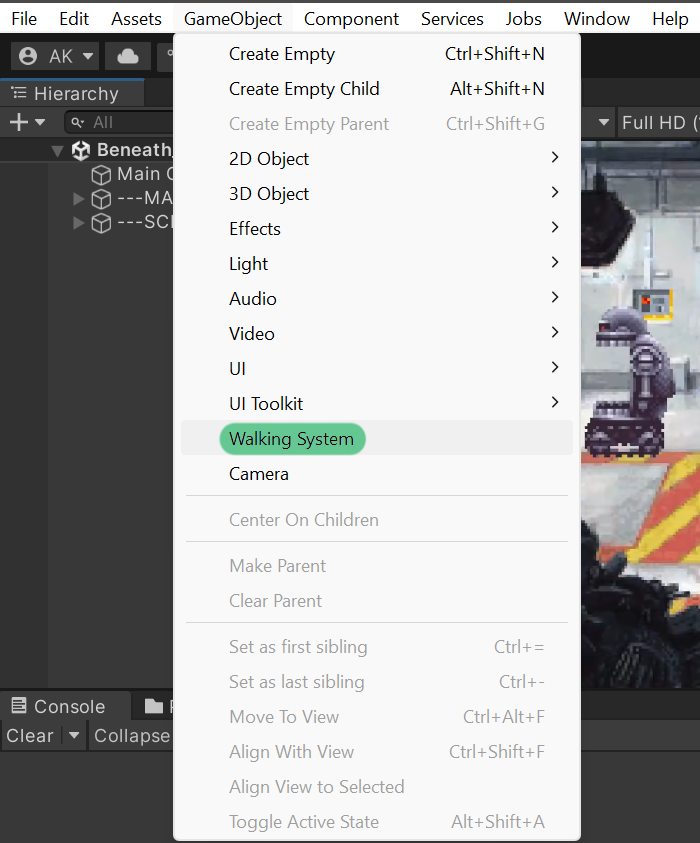
\includegraphics[width=.5\linewidth]{img/User doc/walking_system.png}
\caption{Access to new Walking System prefab instance.}
\label{fig:Manual-WS}
\end{figure}

The framework provides its own default implementation of the prefab which contains a \verb|GameObject| with \textbf{Walkable Map} script attached to it as a component. The prefab also comes with a polygon that describes the walkable area accessible to characters. In Figure \ref{fig:Manual-WM}, we can see Unity inspector for the Walkable Map component together with a possible use of this component in scene BaSS. An important part of the walking system is the possibility to create obstacles for the player. To do that, the user can simply press at the \textit{Build new polygon obstacle} button, which generates a new \verb|GameObject| with the \textbf{Polygon} component script attached to it (see Figure\ref{fig:Manual-Polygon}). To remove this obstacle from the walking system, one can simply press a button \textit{X} next to the desired polygon in the list of obstacle polygons. 

Below that, there are options to constrain the starting or the ending points inside the walkable area and outside the obstacle polygons. In other words, if the player clicks on a point outside the walkable area defined by the developer and the option \textit{End Main} is true, then the system will find the closest possible point in the walkable area from the position of the mouse and will move the character to that point. On the other hand, if false is selected, the character will not move as there is no viable path to the position of the mouse click. Similar rules apply to the \textit{End Obstacles} option, where if a mouse click is registered to be inside an obstacle polygon, the closest possible accessible position is found in the walkable area. The \textit{Start Main} and \textit{Start Obstacle} options work similarly but for the starting position, meaning the character. If the character finds itself to be outside the walkable area and the option Start Main or Start Obstacles is selected, the character will try to find a way to the given position, otherwise not.

Finally, the component also contains some visual enhancements for the developer. It is possible to visualise the graph created by the polygons and the character with the option to select a desired colour for the graph. At the very bottom, there is an option to quickly show or hide all edges and points of all polygons contained in this walking system. 
\begin{figure}[H]
\centering
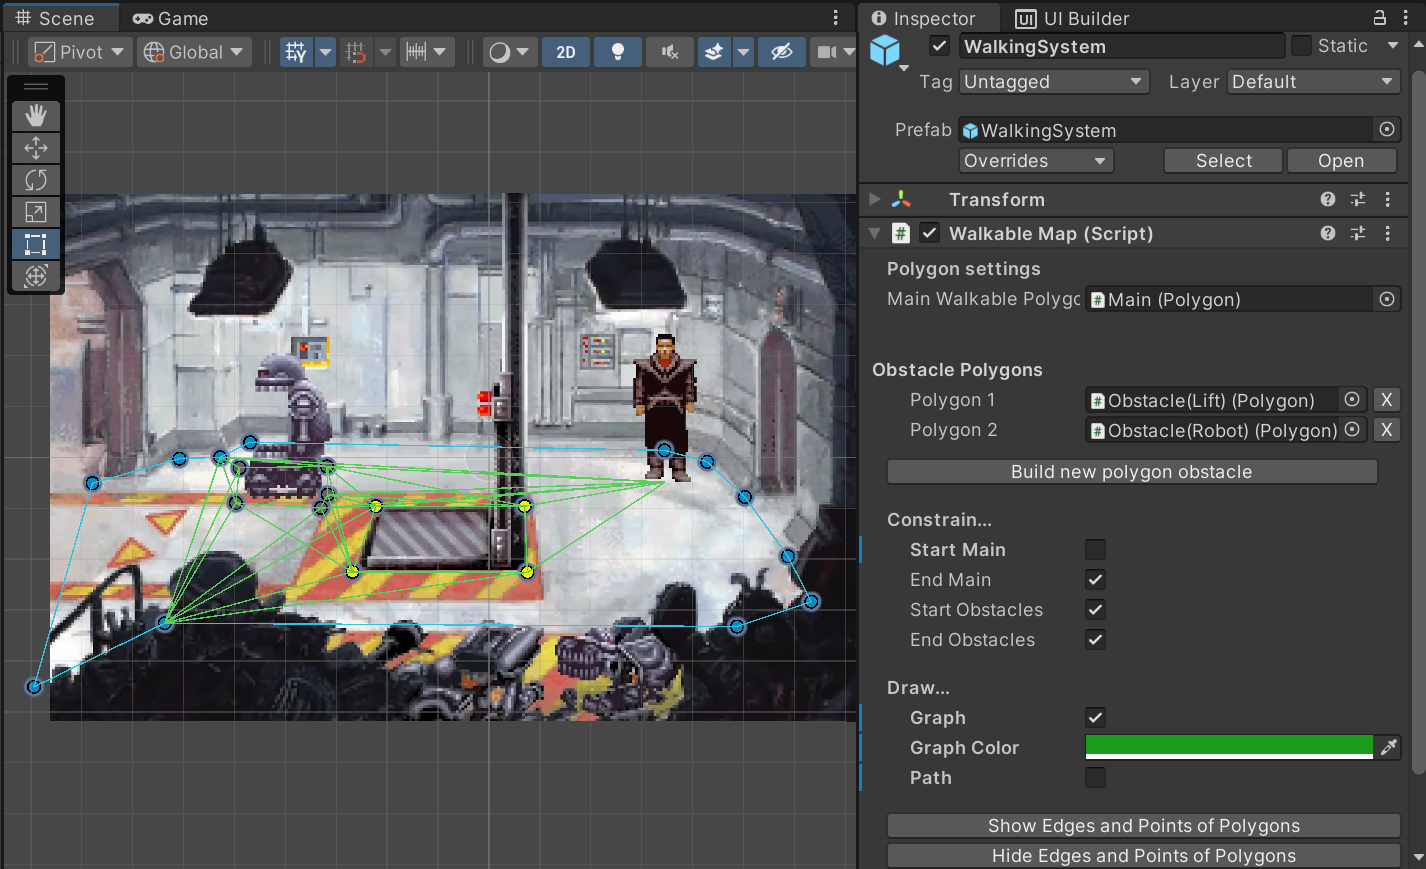
\includegraphics[width=1\linewidth]{img/User doc/walkable_map.png}
\caption{Walkable Map inspector}
\label{fig:Manual-WM}
\end{figure}

The Figure \ref{fig:Manual-Polygon} shows an example of an obstacle polygon. The inspector provides some basic visual adjustments to help the workflow of the developer. These settings include the visibility of the edges and points together with a colour that can be set easily to visually distinguish different polygons from one another. One option also includes the sizing of the points together with a possibility to turn off automatic zooming. \textit{Automatic zooming} (depicted in Figure \ref{fig:Manual-Zoom}) makes the points change size based on the zoom level of the scene. If turned off and zoomed in, the points become very large and the screen is unreadable, so this option is turned on by default.

Undoubtedly, the developer needs to adjust the position and the number of nodes. When the given polygon is selected in the hierarchy, position handles can be seen on top of the vertices of the polygons. These enable easy and intuitive editing of points without the need to individually click on each point \verb|GameObject| in the hierarchy. If the developer then wishes to add a new point, they can simply click on the circle in the middle of the line between two already present points. A new point \verb|GameObject| with the component \textbf{Point} is then created in the exact position of the circle. If a point needs to be deleted, the user needs to press Ctrl key and click on the given point. If done so, the point is removed and a new line edge is formed between the two neighbouring points.
\begin{figure}[H]
\centering
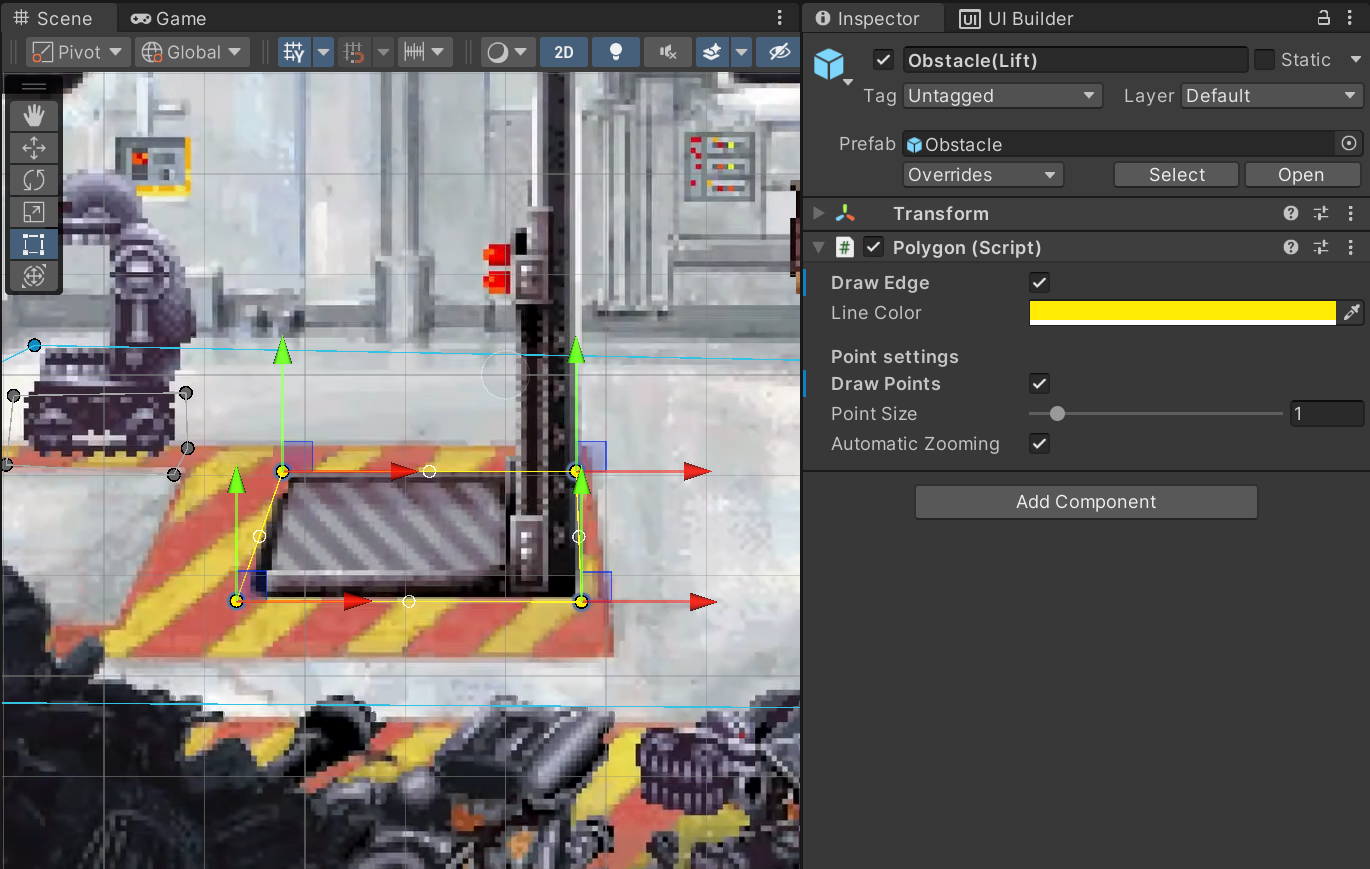
\includegraphics[width=1\linewidth]{img/User doc/polygon.png}
\caption{Polygon inspector}
\label{fig:Manual-Polygon}
\end{figure}

\begin{figure}[H]
\centering
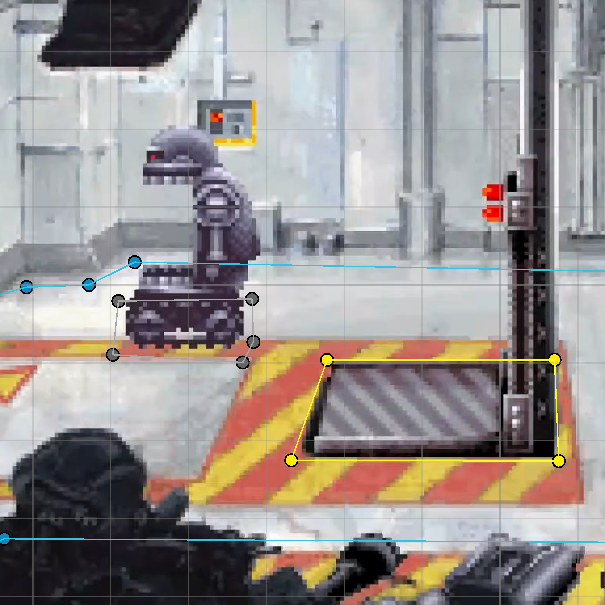
\includegraphics[width=.48\linewidth]{img/User doc/point_scaling.png}
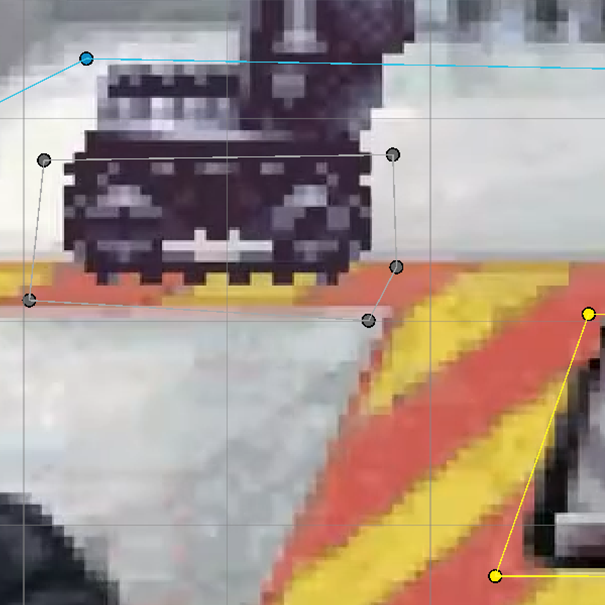
\includegraphics[width=.48\linewidth]{img/User doc/point_scaling2.png}
\caption{Point scaling based on zoom level.}
\label{fig:Manual-Zoom}
\end{figure}
The last two components of the walking system are \textbf{Character Movement} and \textbf{Sprite Scaler} scripts, whose application in the framework can be seen in Figure \ref{fig:Manual-ChM&SS} for TSoMI. 

\textbf{Character Movement} is attached to the player \verb|GameObject| or possibly to any other character that needs to move in the given walking area. The script needs to get a reference to the walkable map and the desired speed of movement can also be adjusted. An end point can also be given and is mainly for debugging purposes. If defined, the graph in the walkable map component can display a path between a starting point (character) and the ending point without the need to start gameplay. The user can move the end point object around the screen and check if the polygons are adjusted properly.

Finally, the \textbf{Sprite Scaler} component takes care of scaling the sprite of the object to which the component is attached. There are multiple options to choose from. The first option is \textit{None}, meaning no scaling is applied to the character. The other two options are \textit{X }and \textit{Y-based scaling}, where the scaling occurs based on the X or Y axis. The two borderline cases need to be selected, which define the scale the very top and bottom for Y axis or very left and right for X axis of the walkable area. The type of perspective can be also selected. If the \textit{Linear} option is enabled, the character scales linearly. The \textit{Hyperbolic} option provides more variety with the rate of scaling. The last scaling type is \textit{Custom}, which takes the scaling factor in each point in the component \textbf{Point} of the walkable polygon and interpolates between them based on the distance.
\begin{figure}[H]
\centering
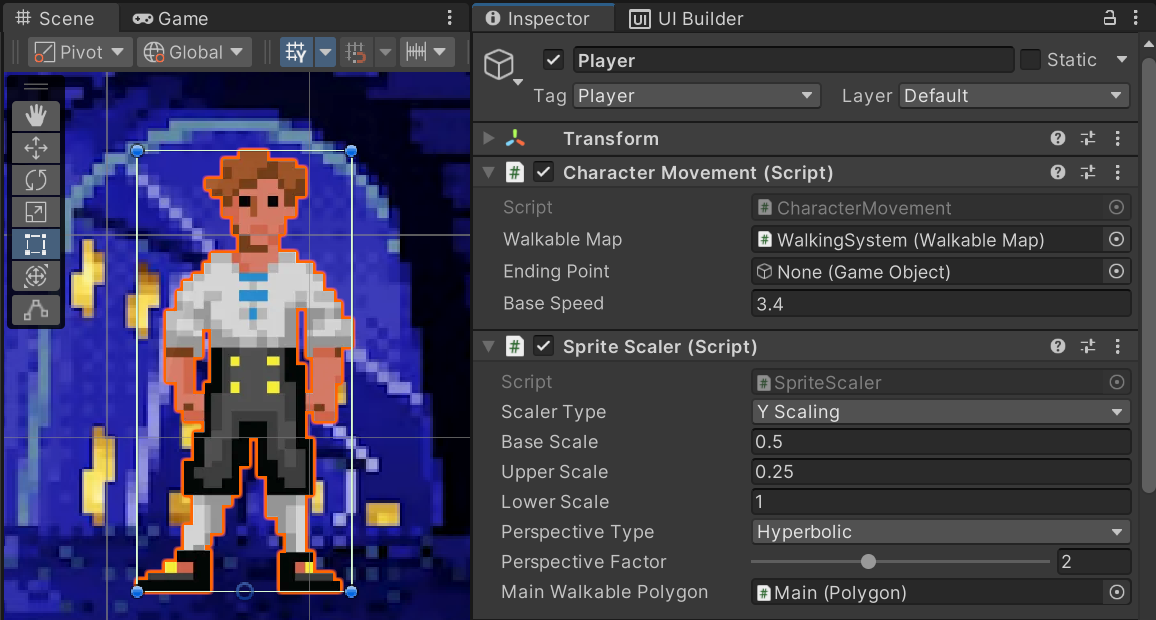
\includegraphics[width=0.8\linewidth]{img/User doc/character_movement.png}
\caption{Character Movement and Sprite Scaler inspector.}
\label{fig:Manual-ChM&SS}
\end{figure}

\subsection{Command System}
The command system contains script \textbf{Command Manager}, which can be attached to a \verb|GameObject| as a component (see Figure \ref{fig:Manual-CM}). It takes the player \verb|GameObject| as a reference to apply action like walking to the appropriate location. The other two following properties \textit{Action Temp} and \textit{Action Sequence} are for debugging purposes as they display the currently hovered over object and the other game object that the player has interacted with.

The next section \textit{Commands} serves as a place to set the behaviour of commands. The list of all possible commands is defined in \textit{Commands List}. A new entry can be added using the button \textit{Add Command}, while an old one can be deleted using the \textit{X} button next to it. Above, there is a property displaying the currently selected command for debugging. Then there are \textit{Default Command} and \textit{Move Command} options. The former decides what the currently selected command will be after the action with the current one is over. The latter defines the command that detects and reacts to movement when clicked on the screen.

The \textit{Set Sentence Structure} option lets the developer define the structure which the command needs to follow when the command sentence needs to be displayed.

Finally, the \textit{Default Actions} let the developer set up what happens if all possible actions for an object given the command are invalid. This is useful when the developer wants to indicate that the the given input from the player is not correct and something else needs to be done. 

\begin{figure}[H]
\centering
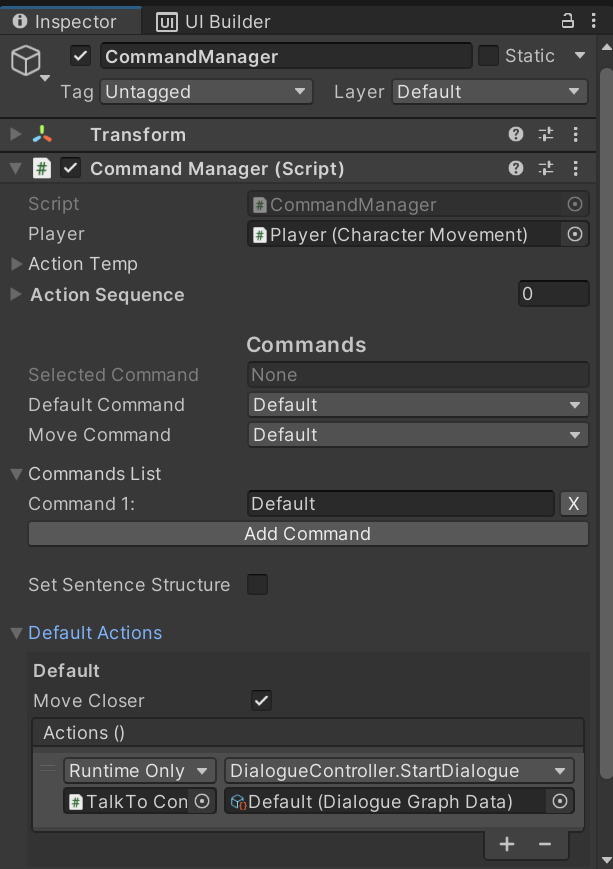
\includegraphics[width=.6\linewidth]{img/User doc/command_manager.png}
\caption{Command Manager inspector.}
\label{fig:Manual-CM}
\end{figure}
\todo{divide into multiple pictures}

In order to create an interactable object in the scene, the user first needs to create a scriptable object in the Assets folder by pressing right click and selecting \verb|Create > Item > World Item|. Here, the user can define the name as well as the description of the item. This asset helps to reference the item throughout the whole project, even in other scenes. Features like the sprite or what the item does when interacted with needs to be set in the \verb|GameObject| with the component \textbf{World Object} attached to with a possible implementation in Figure \ref{fig:Manual-WO} from the BaSS scene. The script takes a \textbf{World Item} asset as a reference in order to assign the item with the actions defined. Except for an option to show a tag with a name of the object, the script also offers a way to define the position of the player when interaction is initiated. The can define multiple of these so-called Go To Points using 2D vector coordinates and during runtime the closest of them is chosen. If none are defined and the character is ordered to move to that position, it selects the position of the object itself. If the object changes position (it is a moving character, for example), the user can define if the position of these points is relative to the object or not. There are also visual settings like selecting a colour and the size of the circle defining the point.
\begin{figure}[H]
\centering
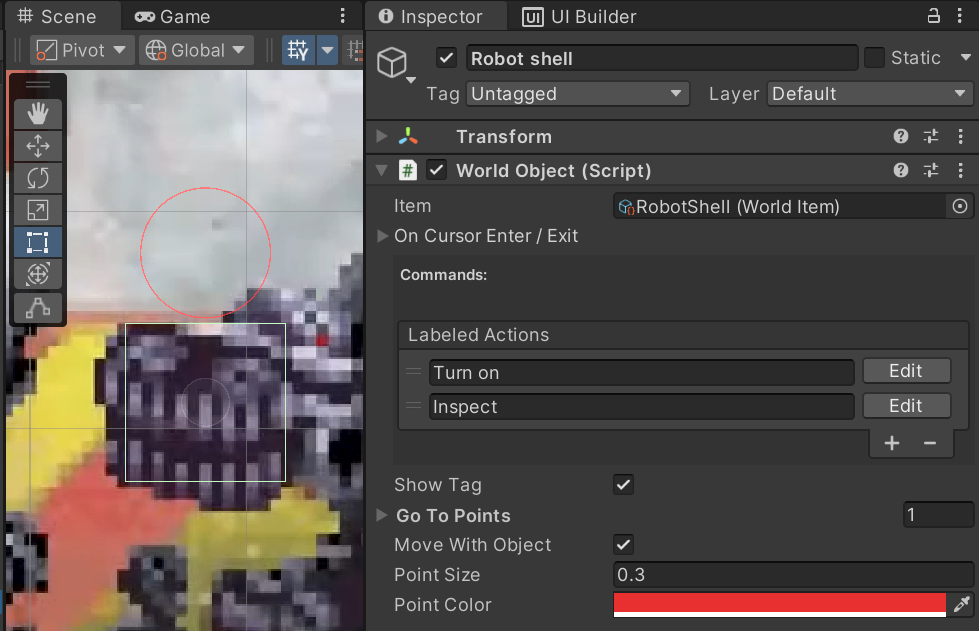
\includegraphics[width=.8\linewidth]{img/User doc/world_object.png}
\caption{World Object inspector.}
\label{fig:Manual-WO}
\end{figure}

The desired behaviour can be created in the reorderable \textit{Labeled Actions} list. If the player interacts with the given object, the command system goes one by one in the list and if all required conditions are met, the given action is executed.
When creating a new action using the \textit{+} button, the user can set a label to that action. This label is purely visual and serves to make the editing of actions readable. When the \textit{Edit} button is pressed, a window pops up, which serves to create the logic of an action. The window first starts with \textit{Previous Interactables}. If enabled, the action is required to contain the same actions as the player had previously interacted with, which can be seen in \textit{Action Sequence} in \textbf{Command Manager}. The next step in verification are \textit{Conditions}, which is a list of \verb|ScriptableObject| \textbf{Variables}, which can be created in the Assets folder through the \verb|Create > Variable > ...| option. This lets the user define either an integer, a float, a string or a boolean variable. In the action window, the conditions need to be given the expected value. If the \textit{Conditions} or the \textit{Previous Interactables} do not match, the action is considered invalid and the next action in the list is checked. In case everything matches, the \verb|UnityEvents| from the very bottom of the window are called based on the type of the click.

\begin{figure}[H]
\centering
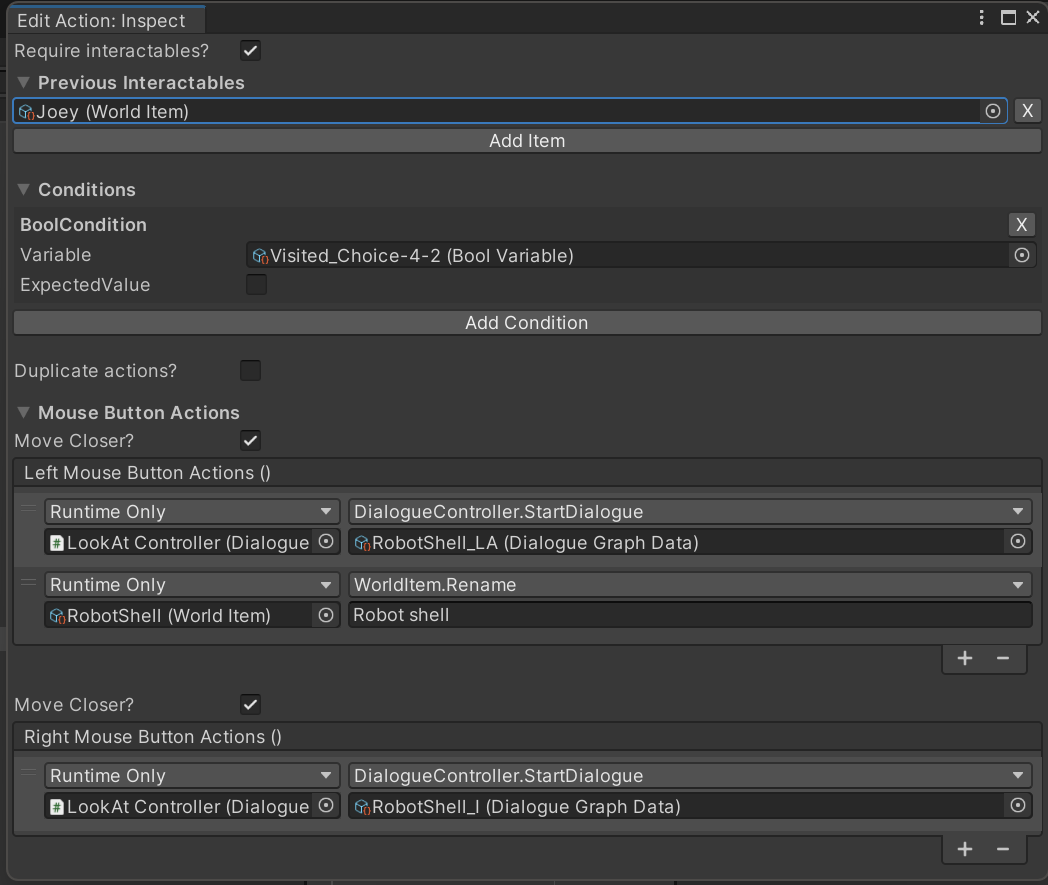
\includegraphics[width=.8\linewidth]{img/User doc/action_window.png}
\caption{Action window.}
\label{fig:BaSS-manual}
\end{figure}

\todo{add inventory interactables}

\subsection{Inventory System}
The inventory system provides the necessary functionalities to manage and display the inventory. Figure \ref{fig:Manual-Inventory} presents a possible use of the \textbf{Inventory Manager} script, which takes care of basic functionalities like taking and removing objects from the inventory. The component can be attached to the player and has the option to define the limit of items that can be picked up. Finally, the user can define the contents of the inventory in the list called \textit{Inventory}. It contains entries of type Inventory Item, which can be defined in the Assets folder by pressing right click and selecting \verb|Create > Item > Inventory Item|. The newly created scriptable object can be given a name, description, as well as rendering data such as a sprite if the icon of the inventory item is meant to be displayed. The newly created item can be dragged as a new entry into the inventory.
\begin{figure}[H]
\centering
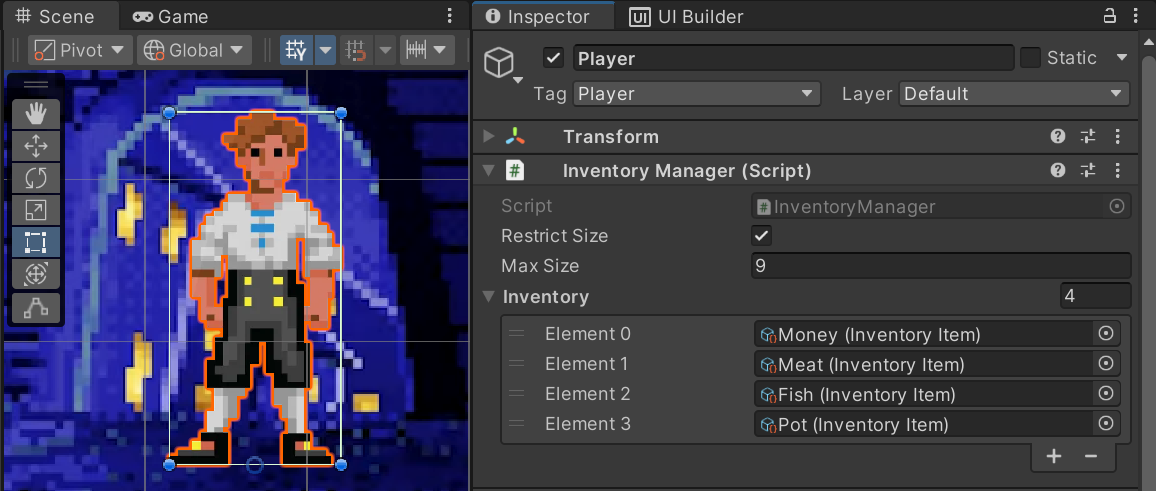
\includegraphics[width=.8\linewidth]{img/User doc/inventory.png}
\caption{Inventory Manager inspector.}
\label{fig:Manual-Inventory}
\end{figure}

Another component that takes care of visualising the inventory is \textbf{Display Inventory}. There is an option to set between two types of inventory: \textit{Name} or \textit{Icon}. The former displays the inventory items as a label with the word (or their combination), whereas the latter creates an icon depicting the item. Both of these approaches are used in the BaSS and TSoMI scenes.

Afterwards, the layout settings can be seen. These can adjust the configuration of the inventory slots: the starting location, width, height and more. 

Finally, the \textit{Max Item Count} option sets how many items can be visible at most. It ties directly to the last script in the inventory system called \textbf{Inventory Scroll Button}, which when attached to a \verb|GameObject| lets the user define the behaviour of scrolling through the inventory by pressing an arrow. This exact scenario is used in TSoMI scene.

\subsection{Dialogue System}
The dialogue system provides the necessary tools for creating and managing conversations between characters. Dialogues are represented as dialogue graphs, which can be created in the Assets folder by right-clicking and selecting \verb|Create > Dialogue > Dialogue Graph|. Once opened, the asset displays a dedicated editor window, as shown in Figure \ref{}.

At the top of the window is a panel displaying the file name alongside three buttons. The first, \textit{Save}, stores the current state of the graph. If the window is closed without pressing this button, any unsaved changes will be lost. The second button, \textit{Load}, reloads the last saved version of the graph. This means any edits made since the last save will be discarded. The third button, \textit{MiniMap}, toggles the visibility of a small map in the top-left corner of the editor window, which provides an overview of the graph layout.

To add elements into the graph, the user must press Space key and a new search window will appear. It prompts the user to create either \textit{Node} or \textit{Group}. Selecting the Node option lets the user choose between six different types of nodes:

\todo{add}

If the user chooses to create a new group from the search window via the path \verb|Groups > Base group|, a new box titled \textit{Dialogue Group} will appear in the editor. Nodes can be added to the group by clicking and holding the left mouse button on a node, dragging it into the group area, and then releasing the button. Multiple nodes can be added to a single group, and it is possible to create connections between any nodes, even those outside the group. When a node is part of a group, moving the group box will also move the contained nodes accordingly. To remove a node from the group, the node needs to be dragged outside of the group while holding Shift key. A group can be renamed by double-clicking on its title. 

In order to run a conversation, the scene must contain a \verb|GameObject| with the \textbf{Dialogue Controller} component attached. This component is responsible for initiating the dialogue and also triggers Unity Events defined in its Inspector both at the beginning and at the end of the conversation. 

Using the Dialogue node, the user can associate a line of text with a specific character through a \textbf{CharacterID} asset. To establish the link between a \verb|GameObject| in the scene and ensure that the dialogue text is displayed near the correct character, the \textbf{Dialogue Controller} component provides a list called \textit{Character ID Data}. Each entry in this list maps a \verb|GameObject| (referred to as the \textit{Character}) to a corresponding \textbf{CharacterID} asset (referred to as the \textit{ID}).

The \textbf{Dialogue UI Controller} component allows the developer to assign a specific prefab to be instantiated as the dialogue text box during runtime. Additionally, it provides options in the Inspector for customizing UI elements, such as button colors and other minor interface settings.

\section{Showcase}
To demonstrate the capabilities of our framework, we chose to recreate scenes from two classic point-and-click adventure games: \textit{The Secret of Monkey Island} and \textit{Beneath a Steel Sky}. Both titles are iconic representatives of the genre, released during its golden era, and introduced several innovative features that later became genre standards. While \textit{The Secret of Monkey Island} uses a command-based interaction system, \textit{Beneath a Steel Sky} takes a more context-sensitive approach. The two games also differ in their inventory design and other small UI elements, such as interaction tags and descriptive sentences, making them ideal candidates to test and showcase the flexibility of our framework.

Another reason we selected these specific titles is their age and current distribution status: they are no longer sold as new releases. Works in the public domain can be used freely without restrictions, but since video games are still a relatively young medium, only a few very old titles or special cases have entered the public domain.
Our project is non-commercial and our use of these games falls under fair use for educational purposes, but the boundaries of fair use are not always clearly defined. 
Newer game developers might object to similar use of their intellectual property. We therefore encourage all readers to support the original games where possible. The sequel to \textit{Beneath a Steel Sky} is available on Steam, and \textit{The Secret of Monkey Island} can be purchased as a modern remake.

\subsection{Instructions}
\verb|Attachments.zip| includes the \verb|TSoMI-Build| and \verb|BaSS-Build| folders, which in addition to a few application binaries, a dynamically linked library and directories with the game assets contain an executable file. To run the game, simply run the \verb|TaleCraft.exe| binary. Both games will show a \textit{Made with Unity }splash screen followed by the scene itself. To quit the game, one needs to simply press ESC on the keyboard.

\subsection{Beneath a Steel Sky}
\textbf{Beneath a Steel Sky} showcase takes place in a starting location of the original game. The style of the following instructions are taken from the original manual for the game \cite{BaSS-Manual}.

\textbf{Clicking} on objects or characters causes the main character, Foster, to interact with them. To \textbf{move} Foster, the player can point the cursor at navigable areas of the screen and click either mouse button. Foster will not walk into walls or inaccessible areas. Certain objects in the game world can be \textbf{examined} or \textbf{interacted} with. These are identified by on-screen tags that appear when the cursor hovers over them. Pressing the \textbf{left mouse button} causes Foster to examine the object, while the \textbf{right mouse button} attempts to pick up or use it. The game selects the most logical action based on context, for example, clicking on a character will typically initiate a conversation. 

When the pointer is moved to the top edge of the screen, a horizontal bar appears, displaying an \textbf{inventory} with all items currently carried by Foster (see Figure \ref{fig:BaSS-manual}). Interaction with these items follows the same logic as with objects in the game world: \textbf{hovering} the cursor over an item reveals its name, pressing the \textbf{left mouse button} displays a short description of the item, while pressing the \textbf{right mouse} button selects it for further interaction. 

When the cursor hovers over another character, clicking either mouse button initiates a conversation. Dialogue options are presented at the top of the screen and the player can choose a line by clicking on it. 

\begin{figure}[H]
\centering
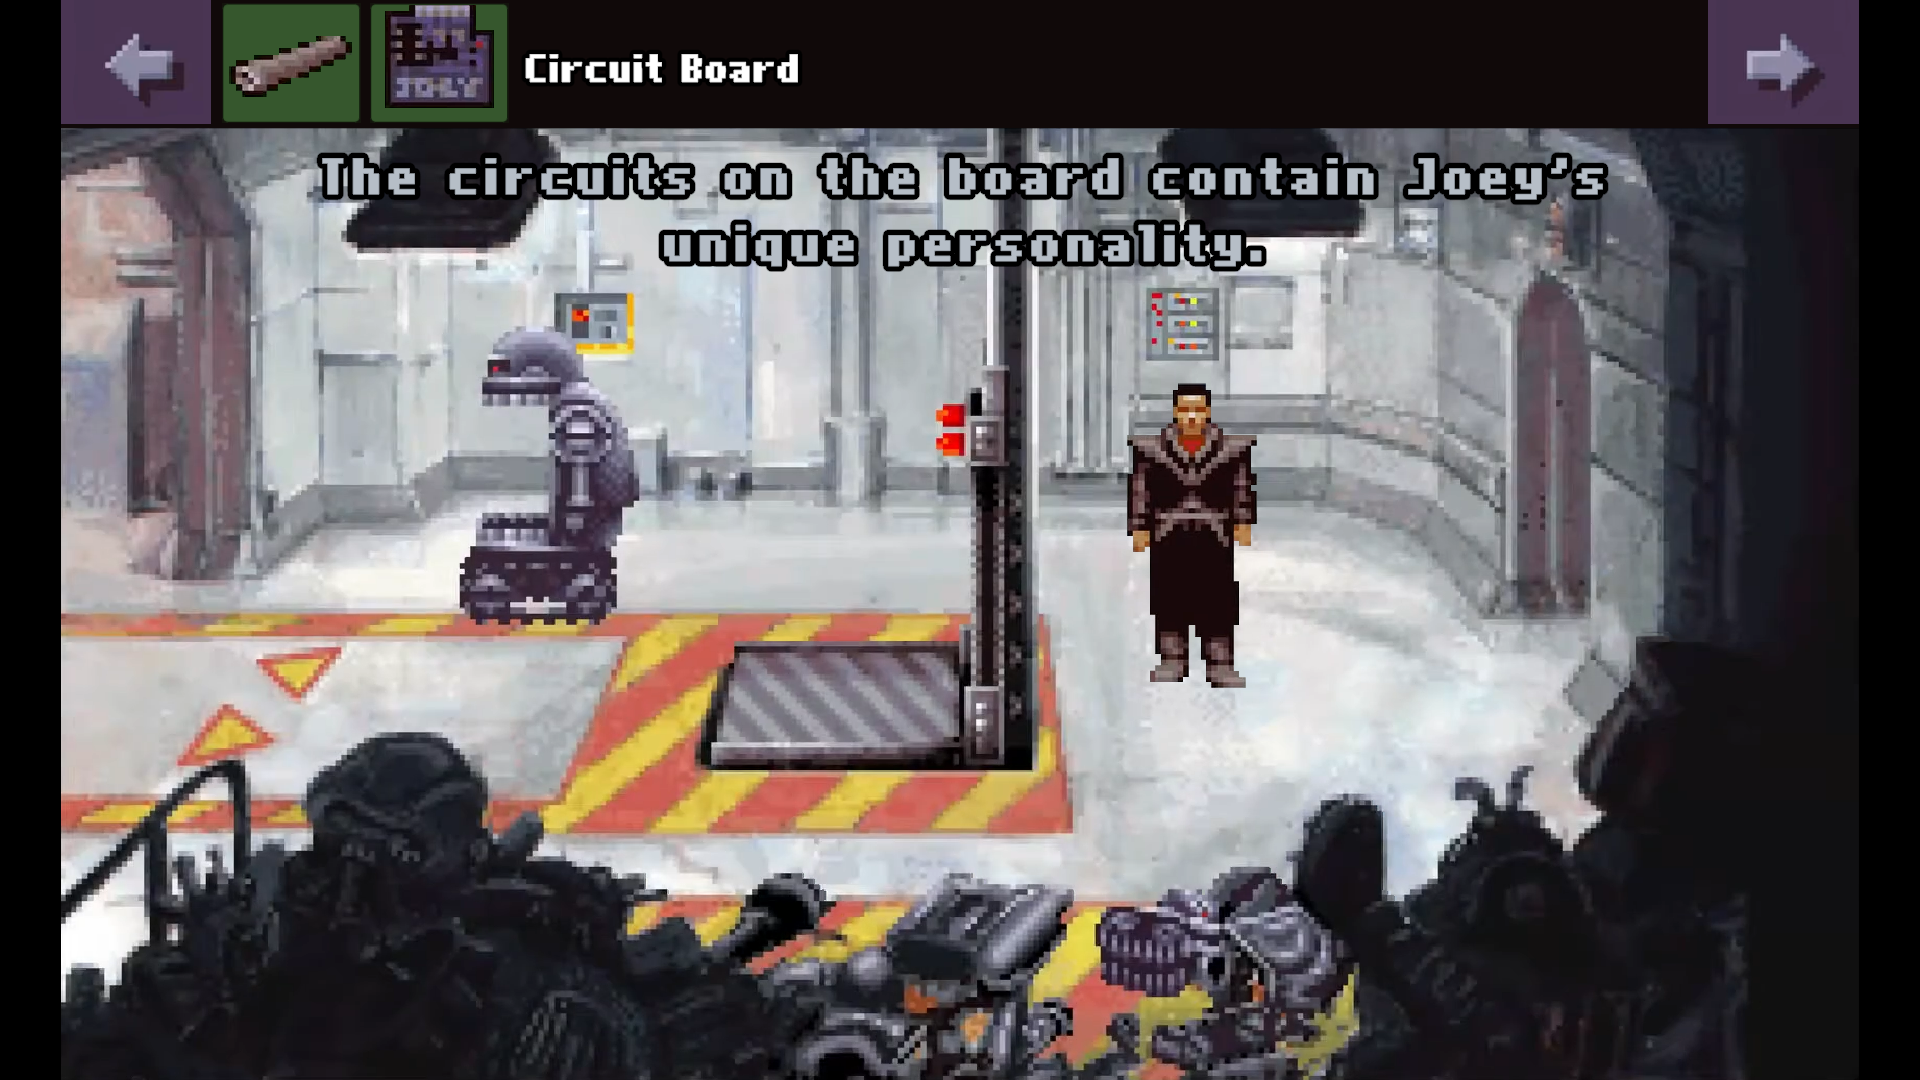
\includegraphics[width=.8\linewidth]{img/manual.png}
\caption{Beneath a Steel Sky (showcase): Screen.}
\label{fig:BaSS-manual}
\end{figure}

\subsection{The Secret of Monkey Island}
The showcase game of The Secret of Monkey Island takes place on a street in the Town of Maleé. The style of the following instructions are taken from the original manual for the game \cite{TSoMI-Manual}.

\subsubsection{Screen}
The game screen is divided into multiple visually distinct parts (see Figure \ref{fig:TSoM-manual}):
\begin{enumerate}
    \item \textbf{Animation window} is the largest area of the screen and serves as the main stage where the action occurs. It displays the current location the protagonist, Guybrush, is currently in. All character dialogue and game-related messages are also displayed in this window. 
    \item Located directly below the Animation window, the \textbf{Sentence} is where players construct simple commands that guide Guybrush's actions. A typical sentence includes a verb and one or two objects. For example, a valid command might be: “\verb|Look at poster.|”
    \item \textbf{Command verbs} are listed in columns underneath the Sentence. Players select verbs by hovering the cursor over them and clicking the left mouse button.
    \item The \textbf{Inventory} is located to the right of the Command verbs section. There is no limit to how many items can carried. When more than six items are in the inventory, arrow buttons appear to allow scrolling through the full list. 
\end{enumerate}

\begin{figure}[H]
\centering
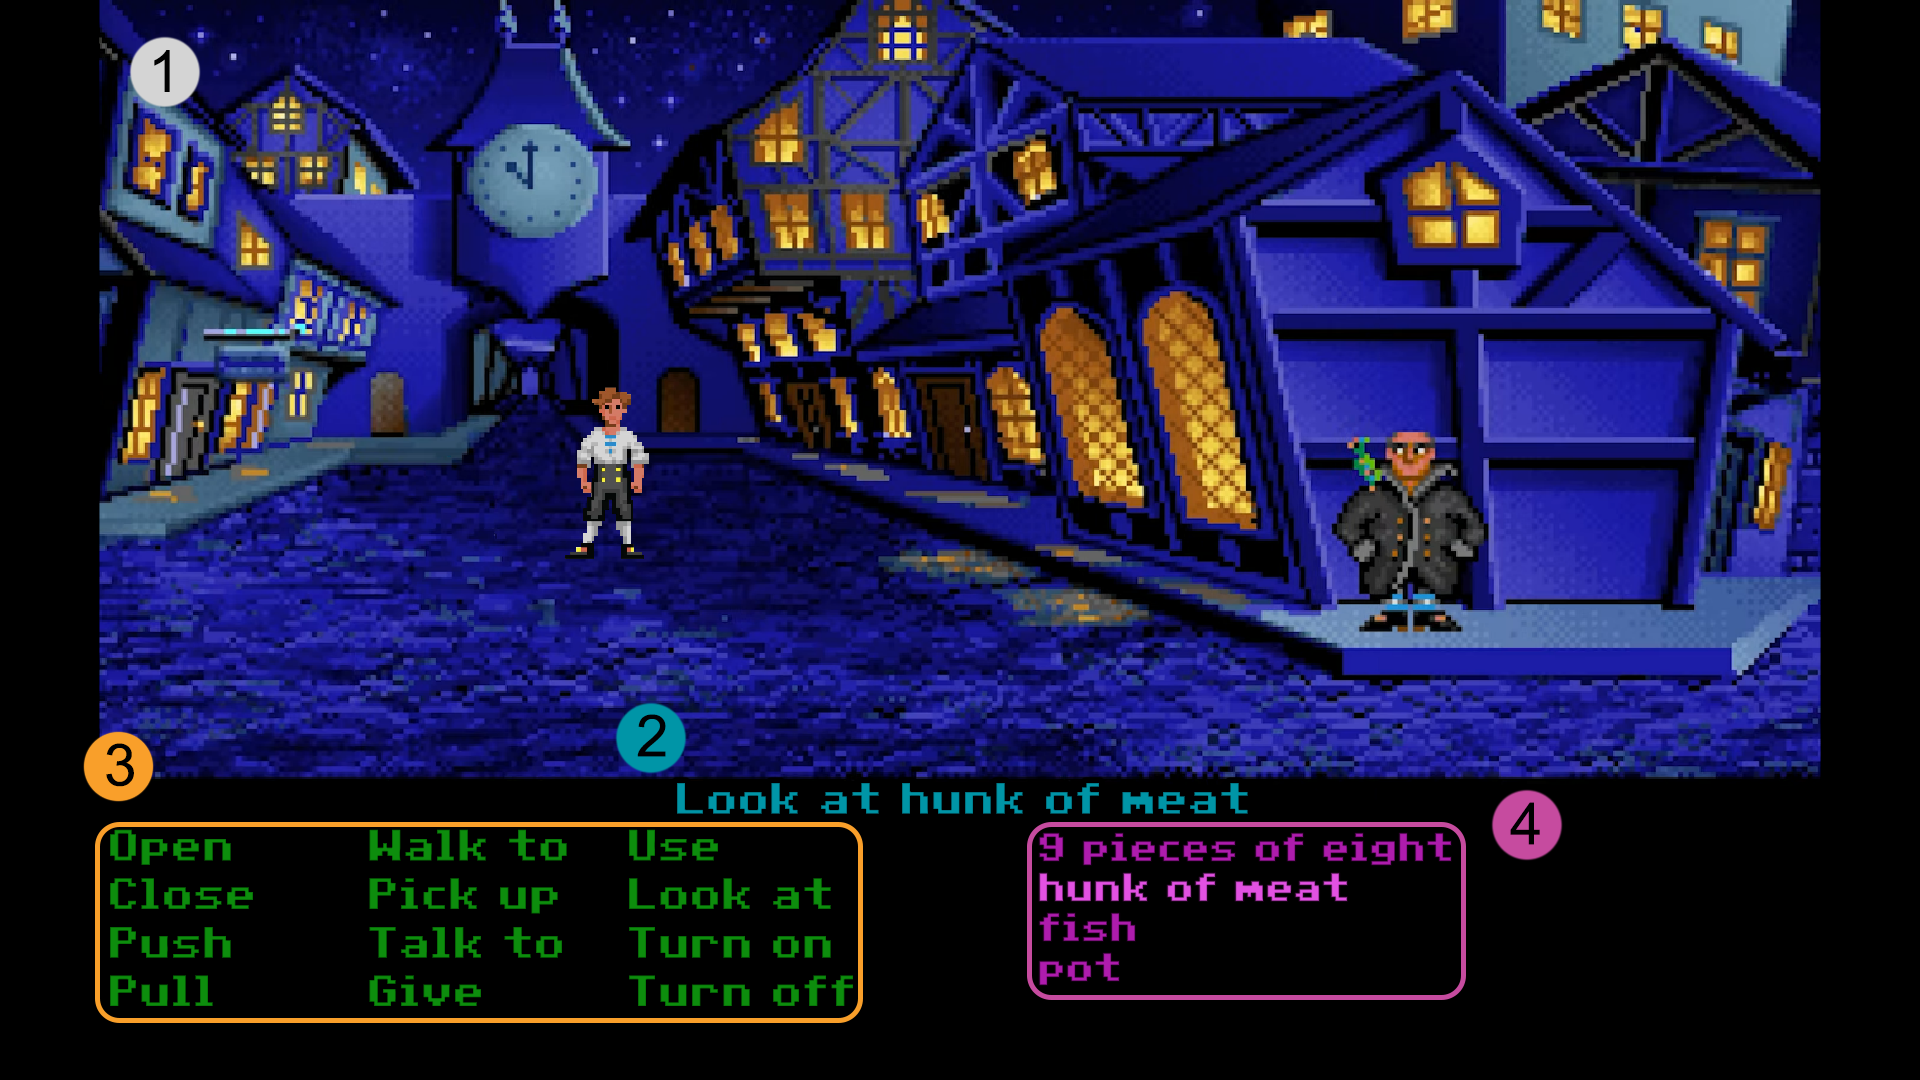
\includegraphics[width=.8\linewidth]{img/tutorial-tsomi.png}
\caption{The Secret of Monkey Island (showcase): Screen.}
\label{fig:TSoM-manual}
\end{figure}

\textbf{Noun Selection and Character Interaction}
Objects, also referred to as nouns, can be selected in two ways. The most common method is by moving the cursor over an object in the Animation window. Most interactive objects in the environment have names, and if an object is usable, its name will appear in the Sentence when the player hovers over it. If no name appears, the object is likely part of the background and serves no gameplay purpose. The objects from the Inventory can be selected directly by clicking on them.

\subsubsection{Movement}
To move Guybrush around the world, the cursor needs to be pointed to the desired location followed by a click. \textit{Walk to} is the default verb in the Command sentence, as moving is the most frequent action players will perform.

\subsubsection{Talking to Characters}
To talk to another character, the player can move the pointer over them and press the right mouse button. During a conversation, dialogue options will appear at the bottom of the screen as seen in Figure \ref{fig:TSoM-manual2}.  The phrase that we want Guybrush to say can be selected by simply clicking on it. What Guybrush says can influence how other characters respond, and new dialogue options may appear as conversations develop.

\begin{figure}[H]
\centering
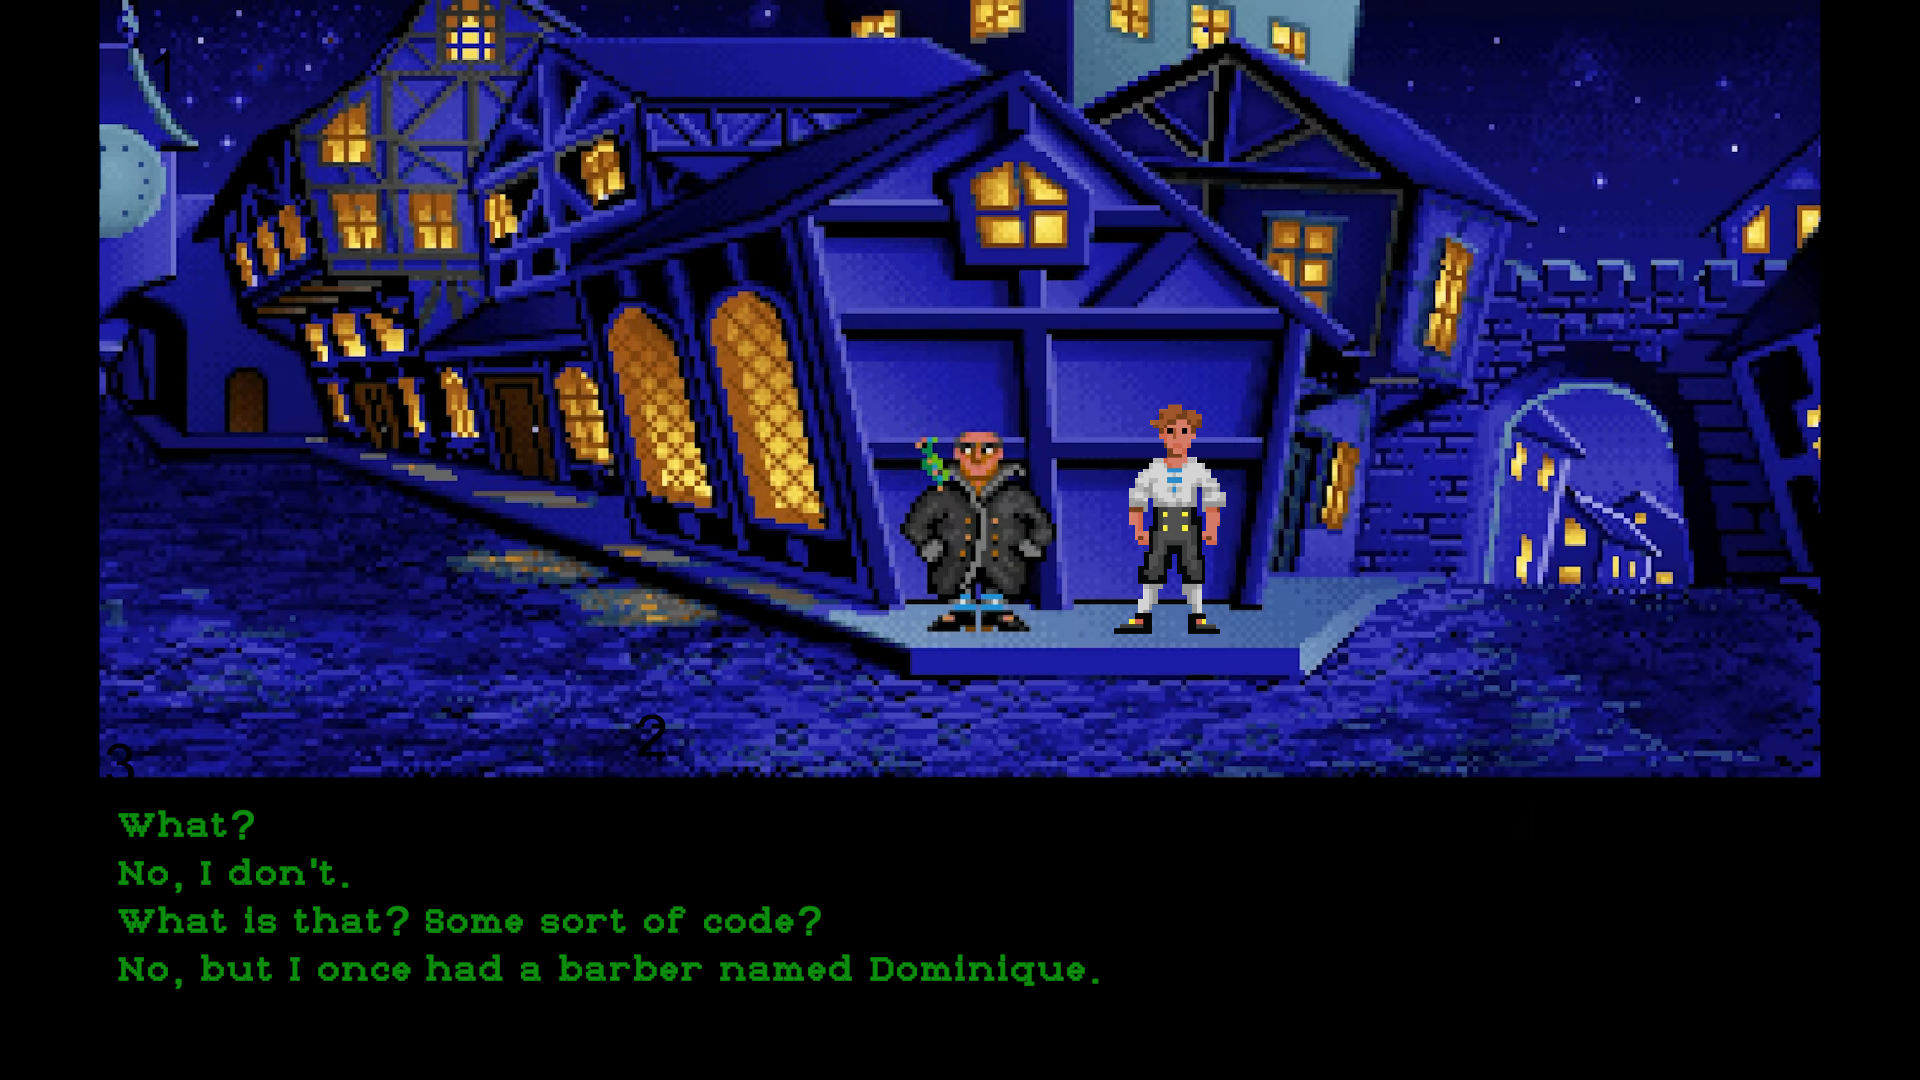
\includegraphics[width=.8\linewidth]{img/manual-tsomi.png}
\caption{The Secret of Monkey Island (showcase): Dialogue.}
\label{fig:TSoM-manual2}
\end{figure}

\chapwithtoc{Conclusion}

In the conclusion, you should summarize what was achieved by the thesis. In a few paragraphs, try to answer the following:
\begin{itemize}
\item Was the problem stated in the introduction solved? (Ideally include a list of successfully achieved goals.)
\item What is the quality of the result? Is the problem solved for good and the mankind does not need to ever think about it again, or just partially improved upon? (Is the incompleteness caused by overwhelming problem complexity that would be out of thesis scope\todo{This is quite common.}, or any theoretical reasons, such as computational hardness?)
\item Does the result have any practical applications that improve upon something realistic?
\item Is there any good future development or research direction that could further improve the results of this thesis? (This is often summarized in a separate subsection called `Future work'.)
\end{itemize}

\chapter{Acknowledgments}

\section{Inspirations}
Michaela Štolová's \textit{UCube - mobilní aplikace pro speedcubing (2020)} \cite{Stolova2020}, Vilém Gutvald's \textit{Tower Defense Game with Procedurally Generated Content and Rogue-like Elements (2024)} \cite{Gutvald2024} and Martin Vejbora's \textit{Carty – Arcade Racing Game (2020)} \cite{Vejbora2020} bachelor theses have been used as a source for inspiration on the thesis structure and content due to the similarity of the subject matter.

\section{Use of AI}
The AI tool ChatGPT-4 has been used during the writing of this thesis to help find a suitable word or expression for sentences to avoid unnatural phrasing. No text has been generated by it directly. It has also been used to try to debug some parts of the project's code.

\section{External Assets}
This project uses assets such as sprites and dialogue text from the classic titles \textit{The Secret of Monkey Island} (1990) and \textit{Beneath a Steel Sky} (1994). The use of these materials is strictly non-commercial and intended solely for educational purposes within the scope of this framework. The creators of TaleCraft do not endorse or encourage unauthorized use of copyrighted content. Instead, we strongly encourage readers to support the original developers by purchasing the official releases. A sequel to \textit{Beneath a Steel Sky} named \textit{Beyond a Steel Sky} is available on Steam \cite{Beyond-a-Steel-Sky}, and \textit{The Secret of Monkey Island} has been rereleased as a modern remake and also can be found on Steam \cite{TSoMI-steam}. 

All other assets used in the project are under creative commons license and are credited in the folders they are stored in.  
\include{bibliography}

\appendix
\include{howto}

% if your attachments are complicated, describe them in a separate appendix
%\include{attachments}

\openright
\end{document}
